% Version 2.1.0 changed 30.11.2014 by GEORGE KRYLOV 

\documentclass{book}
\usepackage[utf8]{inputenc} 
\usepackage[T2A]{fontenc}      
\usepackage[russian]{babel}
\usepackage[dvips]{graphicx}
\usepackage[usenames]{color}
\usepackage[pdftex, colorlinks, linkcolor=black]{hyperref}

\usepackage[left=10mm, top=10mm, right=10mm, bottom=20mm, head=10mm, nofoot]{geometry}

\newcommand{\blackBlueText}{\noindent\bfseries\textcolor[rgb]{0,0,0.6}}
\newcommand{\whiteBlueText}{\textcolor[rgb]{0,0,1}}
\newcommand{\yellowText}{\textcolor[rgb]{1,0,0.8}} % нужно доделать редактору
\newcommand{\greenText}{\textcolor[rgb]{0.5,1,0.8}} % нужно доделать автору
\newcommand{\orangeText}{\textcolor[rgb]{1,0.8,0.1}}

\newcommand{\bC}{\textcolor[rgb]{0,0.1,1}}
\newcommand{\bbC}{\textcolor[rgb]{0.2,0.1,0.75}}
\newcommand{\rC}{\textcolor[rgb]{1,0,0.1}}
\newcommand{\rrC}{\textcolor[rgb]{0.75,0.1,0.2}}
\newcommand{\gC}{\textcolor[rgb]{0.1,0.65,0.2}}
\newcommand{\programm}{\bfseries\noindent\tt}
	
\title{
	\large{\bfseries Инженерный Робототехнический центр ФМЛ №30}\\
	~\\
	~\\
	~\\
	~\\
	~\\
	~\\
	~\\
	~\\
	~\\
	~\\
	\LARGE{\slshape Методическое пособие по Lego Mindstorms для первого года изучения робототехники}
	~\\
	~\\
	~\\
	~
}

\author{
	~\\
	~\\
	~\\
	~\\
	Лузина Е.П.\\
	Лузин Д.В.\\
	Крылов Г.А.\\
	~\\
	~\\
	~\\
}
	
\date{
	Санкт-Петербург\\
	2013
}

\begin{document}
	\maketitle{}
	
	\newcounter{counterPicture}
	\newcounter{counterLesson}
	
	\tableofcontents
	\stepcounter{counterLesson}
	\renewcommand{\chaptername}{Занятие}
	
	{\LARGE\bfseries Введение}\\\\

Последний этап данного курса~--- это выполнение самостоятельного проекта командой учащихся. Работая над проектом, помимо конкретных технических результатов дети учатся следующим универсальным умениям:

\begin{itemize}
	\item ставить стратегическую цель (отдаленную по времени, но значимую) и разбить ее на тактические шаги;
	\item оценивать имеющиеся ресурсы, в том числе собственные силы и время, распределять их;
	\item добывать информацию, критически оценивать ее, ранжировать по значимости, ограничивать по объему, использовать различные источники, в т.ч. людей, как источник информации;
	\item планировать свою работу;
	\item выполнив работу, оценить ее результат, сравнить его с тем, что было заявлено в 
	\item качестве цели работы;
	\item увидеть допущенные ошибки и не допускать их в будущем.\\\\
\end{itemize}

В рамках нашего курса учащимся предлагается групповая форма проектной деятельности, имеющая следующие преимущества:

\begin{itemize}
	\item в проектной группе формируются навыки сотрудничеств;
	\item проект может быть выполнен наиболее глубоко и разносторонне;
	\item на каждом этапе работы, как правило, есть свой ситуационный лидер. Каждый, в зависимости от своих сильных сторон, включается в работу на определенном этапе;
	\item в рамках проектной группы могут быть образованы подгруппы, предлагающие различные пути решения проблемы, идеи, гипотезы, точки зрения. Элемент соревновательности повышает мотивацию и позитивно сказывается на результате.\\\\
\end{itemize}

На заключительном занятии кружка проводится защита всех проектов в формате  научной конференции с докладами. Учащимся будет предложено проанализировать свою деятельность и деятельность своих товарищей (подробнее см. Занятие~\ref{lesson29}).

После защиты учащиеся могут выступить со своими проектами на соревнованиях и конференциях различного уровня  (список см. Приложение) и получить внешнюю оценку своей деятельности.

Строение занятий 23--29 немного отличается от других занятий в данном пособии. По умолчанию во всех этих занятиях ведется самостоятельная работа команд по проектам. Каждое занятие выделяет определенный этап в развитии проекта учащихся, позволяет преподавателю подробнее остановиться на анализе различных аспектов проектной деятельности. Важно отметить, что в зависимости от уровня подготовки группы каждый этап может потребовать не одного, а двух или даже трех занятий. 

В каждом занятии есть основные результаты данного этапа, конкретный нюанс проектный деятельности на который следует обратить внимание и примеры деятельности учащихся на данном этапе. Часть разделов написаны только  для преподавателя, для его подготовки к занятиям этого этапа,  в таком случае в плане урока им выделено 0 минут. 

Главное, от чего следует отталкиваться~--- это деятельность конкретных команд на занятии, всесторонняя помощь и направление учащихся.\\\\
~\\\\
~\\\\
\noindent Авторы:\\\\
\indent Лузина Екатерина Павловна\\
\indent Лузин Дмитрий Валерьевич\\
\indent Крылов Георгий Андреевич\\
	\chapter{Что такое робот}
{\bfseries Анонс:}\\\\
Техника безопасности. Исторический обзор развития робототехники. Обзор-викторина кинороботов. Классификация роботов. Практикум «Фантазийный робот».\\\\
{\bfseries Цели:}
\begin{itemize}
	\item{}{\bfseries Обучающие:} Связать общие представления учащихся о роботах, полученные из книг и фильмов с содержанием спецкурса. Ознакомить учащихся с  различными видами роботов.
	\item{}{\bfseries Воспитательные:} Познакомить учащихся друг с другом, снизить уровень их тревожности.\\
\end{itemize}	
{\bfseries Ход занятия:}\\\\
\begin{tabular}{lll}
	\hyperlink{lesson1x1}{1. Организационный момент} & Презентация & (5 мин)\\
	\hyperlink{lesson1x2}{2. История робототехники} & Презентация & (20 мин) \\
	\hyperlink{lesson1x3}{3. Роботы из кинофильмов} & Игра & (30 мин) \\
	\hyperlink{lesson1x4}{4. Классификация роботов} & Презентация & (10 мин)\\
	\hyperlink{lesson1x5}{5. «Фантазийный робот»} & Игра & (50 мин)\\
\end{tabular}\\\\

{\hypertarget{lesson1x1}{\blackBlueText{I.Организационный момент}}}\\\\

На первом занятии также рекомендуется обсудить правила посещения и пропусков занятий, собрать контактную информацию (Приложение) и подписать инструкцию по технике безопасности.\\\\

{\hypertarget{lesson1x2}{\blackBlueText{II.   История робототехники}}}\\\\ 

{\slshape Историческая справка может быть расширенна рассказами про древние и средневековые механические устройства с демонстрациями (например, 	\href{http://www.etudes.ru/ru/etudes/stopohod/}{\whiteBlueText{\underline{http://www.etudes.ru/ru/etudes/stopohod/}}}).}

Робот. С одной стороны, это слово, почти неизмененным вошло во все языки мира. С другой~--- более непонятного термина еще поискать. Думаю, большинство из вас представило сейчас некого человекообразного андроида, способного бегать-прыгать-стрелять-сражаться и даже немного думать самостоятельно, но с соблюдением инструкций. Что ж, спасибо писателям-фантастам и Голливуду!

Считается, что первые прообразы роботов относятся к эпохе Древней Греции. Тогда на маяке, сооружённом на острове Фарос, установили четыре позолоченные женские фигуры. Днём они горели в лучах солнца, а ночью ярко освещались, так что всегда были хорошо видны издалека. Эти статуи через определённые промежутки времени, поворачиваясь, отбивали склянки; в ночное же время они издавали трубные звуки, предупреждая мореплавателей о близости берега.

Трое братьев Бану Муса, что по-арабски означает «сыновья Мусы», жили в IX веке в Багдаде. Им были хорошо знакомы труды греческих ученых Герона Александрийского и Филона Византийского, а также индийских, китайских и персидских инженеров. Пользуясь полученными знаниями, братья Бану Муса разработали более 100 различных устройств и приспособлений. По словам писателя Эсана Масуда, среди их изобретений были фонтаны, высота струй которых менялась через определенные интервалы времени, часы, оснащенные разными хитроумными «штучками», и сосуды-автоматы для раздачи напитков, запасы жидкости в которых пополнялись за счет хорошо продуманной системы поплавков, клапанов и сифонов.

Согласно свидетельству историка науки Джима Аль-Халили, сыновья Мусы сконструировали «чайную девушку»,~--- простейший робот-автомат размером с человека. Также они создали музыканта, играющего на флейте, который, «возможно, представлял собой самый ранний образец программируемого устройства».

Машины и автоматы братьев Бану Муса были подобны современным. В то же время, как отмечает Эсан Масуд, «вместо электроники в них в основном использовалась сила давления воды, хотя принцип действия был тем же».

Прообразами роботов были также механические фигуры, созданные арабским учёным и изобретателем Аль-Джазири (1136~-- 1206). Так, он создал лодку с четырьмя механическими музыкантами, которые играли на бубнах, арфе и флейте.
\clearpage
\begin{figure}[h!]
	\begin{center}	
		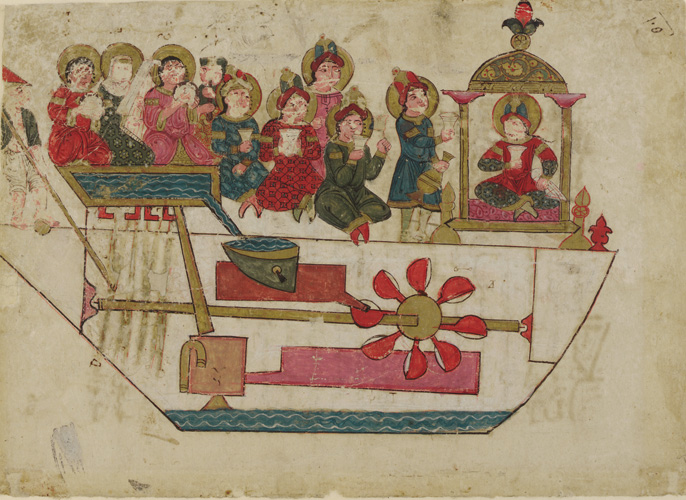
\includegraphics[width=1\linewidth]{chapters/chapter1/images/1}
		\caption{Музыкальная лодка Аль-Джазири.}
		\label{ris:image1x1}
	\end{center}
\end{figure}

Не обошел вниманием создание робота и другой известнейший изобретатель средневековья~--- Леонардо да Винчи. Среди его бумаг найдены разработки человекоподобного робота, одетого в германо-итальянскую броню. Робот был запрограммирован имитировать человеческие движения (приподниматься и садиться, двигать руками и шеей), и имел анатомически правильное строение челюсти. Технология частично основывалась на исследованиях Леонардо в анатомии, в частности Витрувианском человеке. Неизвестно был ли этот проект воплощен в реальность.
\clearpage
\begin{figure}[h!]
	\begin{center}
		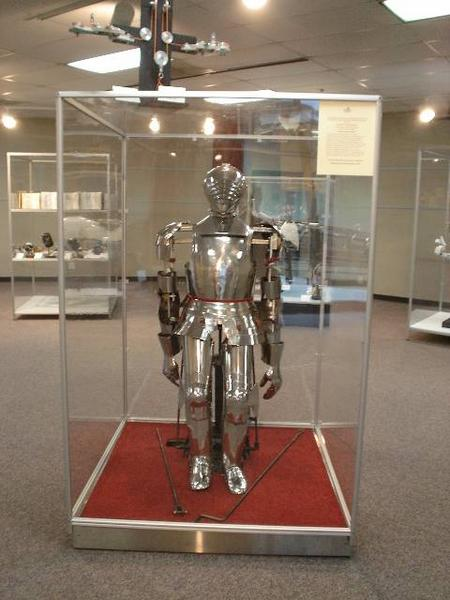
\includegraphics[width=1\linewidth]{chapters/chapter1/images/2}
		\caption{Реконструкция робота Леонардо, выполненная Марио Таддеи.}
		\label{ris:image1x2}
	\end{center}
\end{figure}

Затем были многочисленные автоматические инструменты, танцоры, звери. Выполненные в основном из дерева они могли выполнять десятки различных действий по заложенной программе. Разумеется, ни о какой полезной нагрузке речи не шло, это были  роскошные механизмы, служившие для увеселения богатых граждан.

Век за веком, повторяя общую историю развития техники, появлялись роботы на паровой тяге,  первые электрические роботы, наконец, роботы на полупроводниковой электронике.

{\slshape Если во вступление не включены интерактивные моменты, затягивать его не стоит. После краткого обзора учащимся предлагается следующая викторина.}\\\\

{\hypertarget{lesson1x3}{\blackBlueText{III. Роботы из кинофильмов.}}}\\\\

Викторину можно проводить как для команд, так и для всех учащихся индивидуально. На проекторе демонстрируются кадры из знаменитых фильмов про роботов. По поднятой руке команда (учащийся) получает право ответить на вопрос «Как зовут этого робота и в каком фильме (фильмах) его можно увидеть?». Правильный и полный ответ приносит команде очко, в противном случае право ответа получает следующая по очередности команда.

После того, как робот угадан, рекомендуется показать подготовленные отрывки из кинофильма, на которых хорошо видны конструкционные особенности, возможности и способы передвижения робота и обсудить их с учащимися. 

{\slshape Рекомендации по подобным отрывкам можно найти в Приложении. Ниже представлены возможные варианты вопросов.}
\begin{figure}[h!]
	\begin{center}
		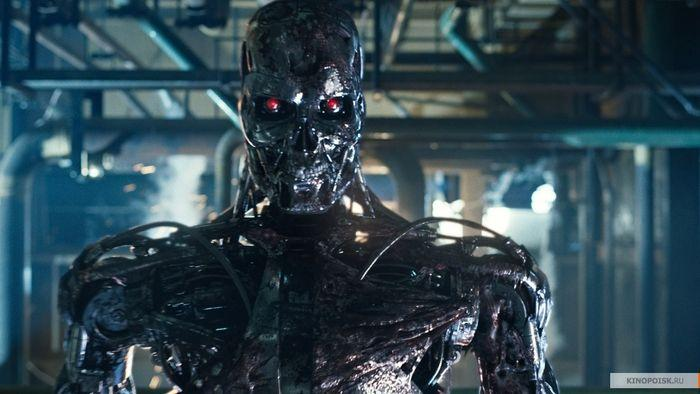
\includegraphics[width=0.98\linewidth]{chapters/chapter1/images/3}
		\caption{Терминатор. Фильмы «Терминатор» 1-5.}
		\label{ris:image1x3}
	\end{center}
\end{figure}
\begin{figure}[h!]
	\begin{center}
		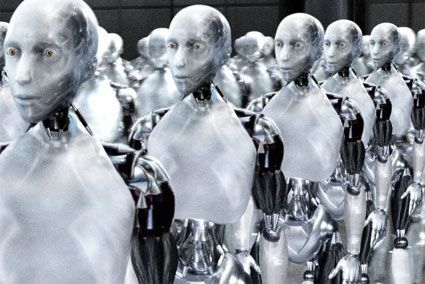
\includegraphics[width=0.98\linewidth]{chapters/chapter1/images/4}
		\caption{Робот Санни. Фильм «Я, робот».}
		\label{ris:image1x4}
	\end{center}
\end{figure}
\begin{figure}[h!]
	\begin{center}
		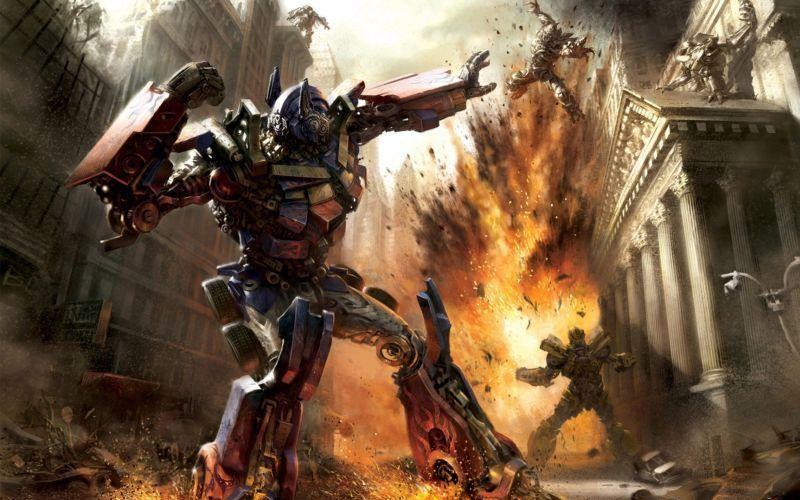
\includegraphics[width=0.98\linewidth]{chapters/chapter1/images/5}
		\caption{Робот Оптимус Прайм. Фильм «Трансформеры» 1,2.}
		\label{ris:image1x5}
	\end{center}
\end{figure}
\begin{figure}[h!]
	\begin{center}
		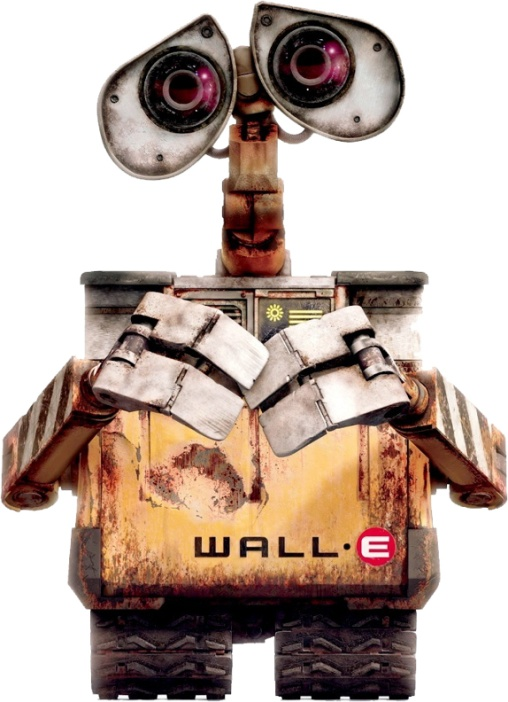
\includegraphics[width=1\linewidth]{chapters/chapter1/images/6}
		\caption{Робот Валли из одноименного фильма.}
		\label{ris:image1x6}
	\end{center}
\end{figure}	
\begin{figure}[h!]
	\begin{center}
		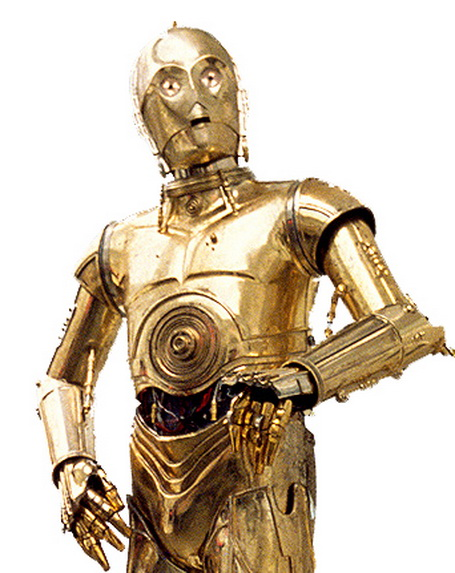
\includegraphics[width=1\linewidth]{chapters/chapter1/images/7}
		\caption{Робот С3РО. Фильм «Звездные войны», 1-6.}
		\label{ris:image1x7}
	\end{center}
\end{figure}
\begin{figure}[h!]
	\begin{center}
		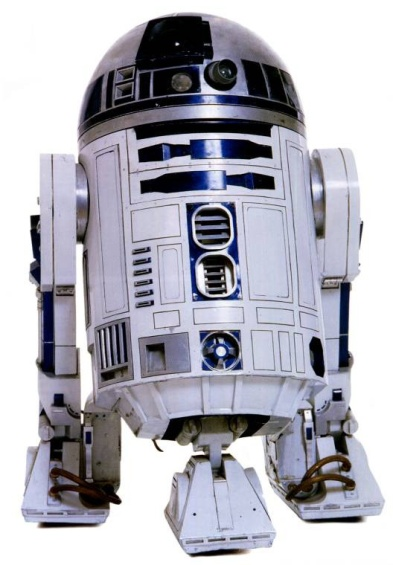
\includegraphics[width=1\linewidth]{chapters/chapter1/images/8}
		\caption{Робот R2D2. Фильм «Звездные войны», 1-6.}
		\label{ris:image1x8}
	\end{center}
\end{figure}
\clearpage
\begin{figure}[h!]
	\begin{center}
		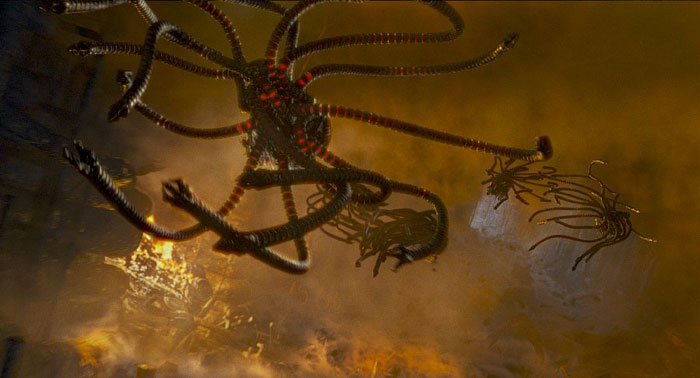
\includegraphics[width=1\linewidth]{chapters/chapter1/images/9}
		\caption{Безымянные роботы-охотники. Фильм «Матрица» 1-3.}
		\label{ris:image1x9}
	\end{center}
\end{figure}	

{\hypertarget{lesson1x4}{\blackBlueText{IV. Классификация роботов.}}}\\\\

Миры ближайшего будущего в кино полны роботов, кажется рукой подать до  эры «настоящих» роботов, роботов-помощников, выполняющих за человека всю тяжелую и нудную работу. Ожидание, правда тянется уже лет 40. Когда же уже роботы будут среди нас? А может быть они уже \dots?

Небезызвестный робот~--- пылесос~--- не робот? А точнейший механический манипулятор, собирающий  машины на заводе~--- не робот? А холодильник, заказывающий недостающие продукты в Интернете? Уже нет?  А  марсоход  Curiosity? Да? А смартфон в вашем кармане? Нет?  Так кто же такой, этот загадочный робот?

На самом деле грани тут, конечно, очень тонкие и условные. И необходимость в классификации роботов и выделении различных направлений робототехники назрела очень серьезная, робототехника еще ждет своего Линнея. В рамках нашего курса мы ограничимся вот такой простейшей классификацией:
\clearpage
\begin{figure}[h!]
	\begin{center}
		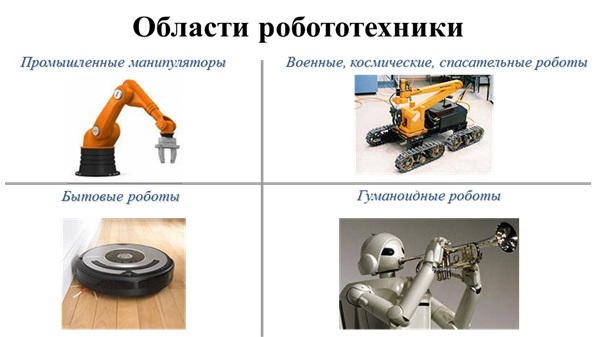
\includegraphics[width=1\linewidth]{chapters/chapter1/images/10}
		\caption{Области современной робототехники.}
		\label{ris:image1x10}
	\end{center}
\end{figure}		

В рамках нашего курса мы коснемся всех направлений. Вы создадите и управляемые, и автономные конструкции. Смоделируете, если не всего человека, то хотя бы его часть. Соберете сложный манипулятор с простым управлением и простую тележку, со сложным поведением. И. конечно, решите самую сложную задачу~--- творческую, создав своего уникального робота. Он будет заваривать чай и приносить тапочки? Имитировать полет мотылька к свету? Или включать дома отопление по SMS-команде? Скоро узнаем!\\\\

{\hypertarget{lesson1x5}{\blackBlueText{V. «Фантазийный робот»}}}\\\\

В заключение первого занятия предлагается провести творческое соревнование по созданию проекта собственного робота. Учащимся предлагается придумать и описать концепцию робота, которого они хотели бы создать. Приветствуются любые рисунки, модели. По желанию допустима как работа в командах, так и индивидуальное творчество.

Дайте толчок к творчеству, предложите детям использовать карандаши, клей, цветной картон, пластилин, пластиковые бутылки, скотч, трубочки для коктейлей, деревянные палочки для шашлыков, канцелярские резинки, пакеты.

На сам процесс творчества отводится примерно 30 минут. В конце проводится краткое представление учащимися своего робота. Вопросы для обсуждения:

\begin{enumerate}
	\item Что делает этот робот?
	\item Как он выполняет свою работу, какие конструкционные особенности ему в этом помогают?
	\item Кому пригодится такой робот?
\end{enumerate}
Можно так же провести голосование и выбрать лучших роботов в следующих номинациях:

\begin{enumerate}
	\item Самый лучший дизайн робота.
	\item Самая продуманная концепция.
	\item Самый нужный человечеству робот.	
\end{enumerate}
{\slshape Материалы, созданные учащимися, сохраните, они еще несколько раз понадобятся в течение курса.}
	\chapter{Знакомство с  Lego Mindstorms NXT 2.0}
{\bfseries Анонс:}\\\\
Lego Mindstorms NXT 2.0. Практикум «Самый длинный мост». Практикум «Неведомый зверь». Терминология.\\\\
{\bfseries Цели:}
\begin{itemize}
	\item{}{\bfseries Обучающие:} Ознакомить учащихся с составляющими набора для создания роботов. Освоить  основные принципы соединения деталей. Обучить учащихся общепринятой терминологии.
	\item{}{\bfseries Воспитательные:} Познакомить учащихся друг с другом, снизить уровень их тревожности.\\
\end{itemize}	
{\bfseries Ход занятия:}\\\\
\begin{tabular}{lll}
	\hyperlink{lesson2x1}{1. Организационный момент} & Презентация & (5 мин)\\
	\hyperlink{lesson2x2}{2. Lego Mindstorms NXT 2.0} & Презентация & (30 мин) \\
	\hyperlink{lesson2x3}{3. «Самый длинный мост»} & Игра & (30 мин) \\
	\hyperlink{lesson2x4}{4. «Неведомое животное»} & Игра & (40 мин)\\
	\hyperlink{lesson2x5}{5. Основы терминологии} & Рефлексия & (5 мин)\\
\end{tabular}\\\\

{\hypertarget{lesson2x1}{\blackBlueText{I.Организационный момент}}}\\\\

Сегодня учащимся предстоит собрать свои первые конструкции и познакомиться с набором. Каждой паре предоставляется свое рабочее пространство, следует проследить, что бы оно было достаточно большим, что бы разместить на нем коробку с деталями и иметь площадку для творчества. Попросите убрать все посторонние предметы со столов, ничего кроме наборов в этот раз не понадобится.

Изначально раздайте учащимся только блоки, моторы и датчики. С одной стороны это позволит им в процессе знакомства с набором держать в руках предметы о которых идет речь, с другой не даст отвлечься на собирание чего-то своего из набора деталей. Набор с деталями следует раздать только в начале упражнения «Самый длинный мост».\\\\

{\hypertarget{lesson2x2}{\blackBlueText{II. Lego Mindstorms NXT 2.0}}}\\\\

Мы будем использовать набор Lego Mindstorms NXT 2.0 8547. В каждом наборе содержится 619 деталей, включая очень мелкие, поэтому, чтобы было легко их находить и хранить нужна четкая система. В качестве кейсов для хранения предлагается использовать следующие коробки для инструментов
\begin{figure}[h!]
	\begin{center}
		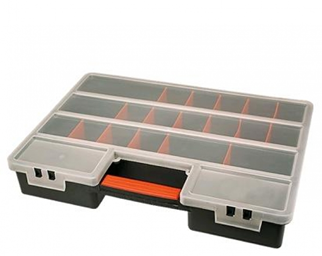
\includegraphics[width=1\linewidth]{chapters/chapter2/images/1}
		\caption{Ящик для хранения деталей.}
		\label{ris:image2x1}
	\end{center}
\end{figure}			

В таком случае удобной оказывается следующая раскладка деталей:
\begin{figure}[h!]
	\begin{center}
		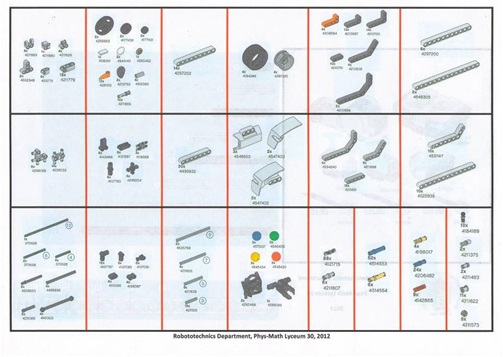
\includegraphics[width=1\linewidth]{chapters/chapter2/images/2}
		\caption{Раскладка деталей набора 8547 (\yellowText{Приложение}).}
		\label{ris:image2x2}
	\end{center}
\end{figure}		

При использовании образовательной версии набора 9797 LEGO MINDSTORMS Education NXT Base Set вкладыш для хранения деталей уже входит в набор.

С другой стороны раскладки удобно напечатать в масштабе 1:1 балки и оси, что бы при переборе наборов просто сравнивать детали с рисунком.
\clearpage
\begin{figure}[h!]
	\begin{center}
		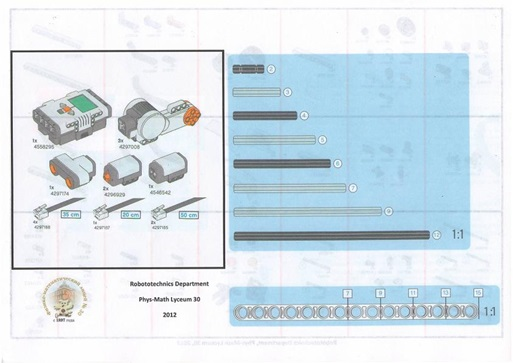
\includegraphics[width=1\linewidth]{chapters/chapter2/images/3}
		\caption{Оборотная сторона раскладки (\yellowText{Приложение}).}
		\label{ris:image2x3}
	\end{center}
\end{figure}		

Заламинированную раскладку деталей рекомендуется вложить в каждый набор. К набору имеет смысл приклеить кармашек, с вложенным листом учета деталей (Приложение).

В конце каждого занятия робот полностью разбирается, все детали раскладываются по местам, а набор сдается преподавателю под роспись. Это позволяет быстро освоить основные моменты конструирования, за счет частой сборки- разборки, а так же повысить ответственность учащихся и уменьшить естественную убыль деталей. Так же коробка с рис. показала себя как удобная в транспортировке при поездках на соревнования в другие города.\\\\	
Помимо деталей конструктора в стандартный набор входят:
\begin{itemize}
	\item Блок NXT. В неформальной литературе так же часто встречается названия брик (brick) и кирпич. На техническом языке  - это 32-битовый микроконтроллер ARM7 256 КБайт FLASH, 64 КБайт RAM  и 8-битовый микроконтроллер AVR 4 Кбайта FLASH, 512 байт RAM, а также беспроводный канал Bluetooth Class II V 2.0. А проще говоря~--- «мозг» нашего робота. К нему будут подключаться все сенсоры (глаза, уши, нос и т.п. робота) и он же будет давать команды моторам (рукам и ногам).
	\clearpage
	\begin{figure}[h!]
		\begin{center}
			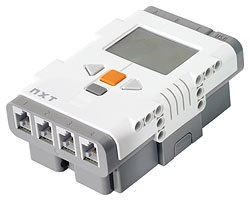
\includegraphics[width=0.65\linewidth]{chapters/chapter2/images/4}
			\caption{Блок NXT.}
			\label{ris:image2x4}
		\end{center}
	\end{figure}	
	
	Блок имеет 3 разъема для подключения моторов (A,B,C), 4 разъема для сенсоров (1,2,3,4) и разъем USB для соединения с компьютером. На передней панели расположен дисплей и 4 кнопки. С помощью оранжевой кнопки можно включить или выключить питание, светло-серые стрелки необходимы при перемещении влево - вправо по меню NXT, а темно-серая кнопка удаляет или возвращает пользователя в предыдущее меню.  На задней стороне блока находится отделение для аккумуляторов. Блок может работать от фирменного аккумулятора Lego, а так же обычных 6 батареек или аккумуляторов типа АА.
	\begin{figure}[h!]
		\begin{center}
			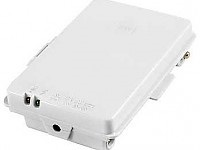
\includegraphics[width=0.65\linewidth]{chapters/chapter2/images/5}
			\caption{Аккумуляторный блок Lego.}
			\label{ris:image2x5}
		\end{center}
	\end{figure}
	
	Так же блок оснащен громкоговорителем, что позволяет проигрывать ему различные звуки при воспроизведении программы.		 
	\item Три сервопривода. Могут вращаться в любом направлении. Скоростью вращения моторов можно программно управлять. В приводы встроен счетчик числа оборотов, точнее градусов на которые повернулся привод.
	\begin{figure}[h!]
		\begin{center}
			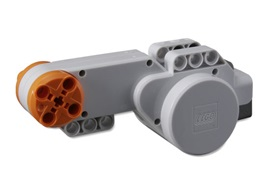
\includegraphics[width=0.6\linewidth]{chapters/chapter2/images/6}
			\caption{Сервопривод.}
			\label{ris:image2x6}
		\end{center}
	\end{figure}
	
	\item Ультразвуковой сенсор. (Особенно любим детьми, после выхода одноименного мультика имеет ласковую кличку Валли). Посылает ультразвуковую волну и принимает ее, отраженную от преграды. По времени прохождения и известной скорости волны определяет расстояние до преграды. Не работает с шероховатыми поверхностями, из-за слишком сильного рассеивания ими звуковых волн.
	\begin{figure}[h!]
		\begin{center}
			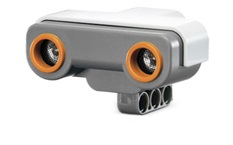
\includegraphics[width=0.6\linewidth]{chapters/chapter2/images/7}
			\caption{Ультразвуковой сенсор.}
			\label{ris:image2x7}
		\end{center}
	\end{figure}
	
	\item Сенсор касания. Просто кнопка. Возвращает состояние нажата/не нажата.
	\begin{figure}[h!]
		\begin{center}
			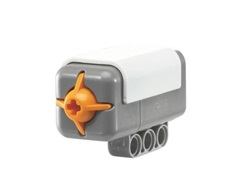
\includegraphics[width=0.6\linewidth]{chapters/chapter2/images/8}
			\caption{Сенсор касания.}
			\label{ris:image2x8}
		\end{center}
	\end{figure} 
	
	\item Сенсор освещенности. Входит в набор Education. Возвращает значение освещенности поверхности в условных единицах от 0 (черное) до 255 (белое).
	\begin{figure}[h!]
		\begin{center}
			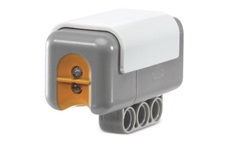
\includegraphics[width=0.6\linewidth]{chapters/chapter2/images/9}
			\caption{Сенсор освещенности.}
			\label{ris:image2x9}
		\end{center}
	\end{figure}
	
	\item Сенсор цвета. Может использоваться в одном из пяти режимов: Lego Color-Red, Lego Color-Green, Lego Color-Blue, Lego Color-RGB и Lego Color. В первых четырех работает как датчик освещенности, подсвечивая себе путь светодиодом соответствующего цвета (цветов). В последнем режиме датчик способен различать цвета.
	\begin{figure}[h!]
		\begin{center}
			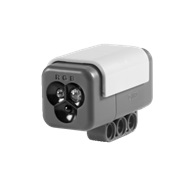
\includegraphics[width=0.6\linewidth]{chapters/chapter2/images/10}
			\caption{Сенсор цвета.}
			\label{ris:image2x10}
		\end{center}
	\end{figure}
\end{itemize}

{\hypertarget{lesson2x3}{\blackBlueText{III. «Самый прочный мост»}}}\\\\

Итак, набор продемонстрирован, правила раскладки деталей оговорены. Самое время для первого практического задания!

Учащиеся разбиваются на группы по 3--4 человека. У каждой группы в распоряжении 1 набор. Задача~--- построить самый прочный мост между двумя столами, находящимися на расстоянии 50 см. Самым прочным считается мост, выдержавший наибольший груз в течение 3 секунд.

{\slshape Возможны вариации на тему «самый длинный мост», «самая высокая башня» и т.д. Главное в этом задании - это возможность детям  после довольно долгого для них обзора, наконец, потрогать набор, попробовать разные варианты соединения деталей, познакомиться друг с другом.}\\\\

{\hypertarget{lesson2x4}{\blackBlueText{IV. «Неведомое животное»}}}\\\\

Учащиеся  разбиваются по парам. Одному человеку в паре предлагается собрать из деталей одного набора любое фантастическое животное за 10--15 минут. Второй участник не должен видеть ни процесса, ни результата (в это время можно предложить ему заполнить информационный лист из Приложения). Затем автору зверя предлагается объяснить своему товарищу, как собрать такого же~--- при этом напарники по-прежнему не видят друг друга и результаты своего труда.

Как правило, в этот момент, по всему классу раздаются диалоги следующего содержания:

- А теперь берешь вот ту серую штучку с пимпочкой и двумя усиками, засовываешь в нее синий треснутый цилиндрик \dots 

-Тот который с колечком или со вштыркой?\\
Возможные результаты подобного творчества представлены на \greenText{рис}.\\\\
\greenText{Рис.}\\\\

Затем следует провести игру еще раз, поменяв напарников ролями.\\\\

{\hypertarget{lesson2x5}{\blackBlueText{V. Основы терминологии}}}\\\\

В конце задания, вместе с учащимися следует проанализировать основную проблему с которой они столкнулись: проблема коммуникации. Для успешной работы в дальнейшем надо договориться о единых названиях для всех деталей. Можно обсудить, что в принципе, названия могут быть любыми, но если мы хотим  в дальнейшем общаться и с другими людьми, стоит выбрать общепринятые названия.

Раздаточный материал: Названия деталей (\yellowText{Приложение}).

Названия стоит проговорить вслух и посоветовать носить с собой раздатку в качестве шпаргалки, пока названия не запомнятся. Впредь использование самостоятельной терминологии рекомендуется аккуратно пресекать.
	\chapter{Знакомство с Lego Digital Designer}
{\bfseries Анонс:}\\\\
Названия деталей. Lego Digital Designer: установка и первые модели.
{\bfseries Цели:}
\begin{itemize}
	\item{}{\bfseries Обучающие:} Закрепить  знание основных терминов. Обучить основам работы в Lego Digital Designer. 
	\item{}{\bfseries \yellowText{\greenText{Развивающие:}}} \\
\end{itemize}	
{\bfseries Ход занятия:}\\\\
\begin{tabular}{lll}
	\hyperlink{lesson3x1}{1. Организационный момент} & Презентация & (5 мин)\\
	\hyperlink{lesson3x2}{2. Названия деталей} & Игра & (15 мин) \\
	\hyperlink{lesson3x3}{3. Lego Digital Designer} & Презентация & (45 мин) \\
	\hyperlink{lesson3x4}{4. Модель совы} & Практика & (50 мин)\\
\end{tabular}\\\\

{\hypertarget{lesson3x1}{\blackBlueText{I.Организационный момент}}}\\\\

Сегодня для работы каждому ребенку понадобятся компьютеры, с установленным на них Lego Digital Designer. Оптимальным является вариант компьютеров, объединенных во внутреннюю сеть, с возможностью создания каждому ребенку личного аrкаунта, блокировки доступа в интернет и к части жесткого диска.\\\\

{\hypertarget{lesson3x2}{\blackBlueText{II. Названия деталей}}}\\\\

Для закрепления материала предыдущего занятия и настройки на рабочий лад предлагается провести следующую игру. В шляпу складываются разные детали набора, из расчета 5--6 штук на одного игрока. У каждого игрока есть 30 секунд, что бы вынимая по очереди из шляпы детали называть их. Назвал правильно~--- получаешь очко, нет~--- кидаешь обратно в шляпу. По истечении 30 секунд шляпа переходит следующему. Игра продолжается пока не закончатся все детали.\\\\

{\hypertarget{lesson3x3}{\blackBlueText{III. Lego Digital Designer}}}\\\\

{\bfseries LEGO Digital Designer (LDD)}~--- это программа, представляющая собой виртуальный конструктор LEGO, с помощью которого можно собирать всевозможные 3D-модели. Как и в реальном конструкторе в {\bfseries LDD} присутствует богатый выбор разнообразных деталей, которые можно скреплять друг с другом. Рабочую область программы можно приближать, удалять и разворачивать под любым углом.

Программа распространяется бесплатно, установочный файл можно скачать с
\href{http://ldd.lego.com/nb-no/download/}{\whiteBlueText{\underline{http://ldd.lego.com/nb-no/download/}}}.
\begin{figure}[h!]
	\begin{center}
		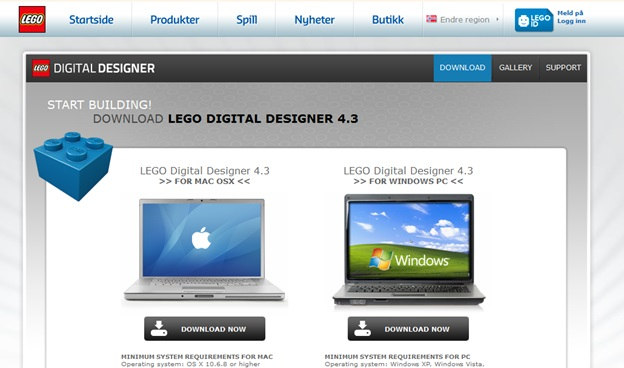
\includegraphics[width=1\linewidth]{chapters/chapter3/images/1}
		\caption{}
		\label{ris:image3x1}
	\end{center}
\end{figure}

Так же версию LDD 4.3 для Windows PC можно найти в папке LDD мультимедийных материалов к настоящему пособию.
\clearpage
Создание моделей  роботов в LDD полезно по следующим причинам:
\begin{itemize}
	\item Прививается навык анализа конструкции. Реальные детали можно соединить абы как, « по вдохновению», но создавая модель придется осознать, как это было сделано.
	\item Прививается навык продумывания конструкции. Создавая дома модель робота к следующему занятию есть возможность перебрать множество вариантов.
	\item Развивается пространственное мышление.
	\item Прививается навык работы в инженерных средах. В настоящем конструировании и роботостроении не обойтись без серьезных расчетов в различных программных пакетах и создания моделей частей устройства. Использование LDD подготавливает детей к работе в подобных программах.
	\item Наличие  сохраненной модели индивидуального проекта позволяет другому ребенку ознакомиться с техническими решениями, использованными в конструкции и, при необходимости, воспроизвести отдельные узлы или всего робота.
\end{itemize}

{\slshape В рамках настоящего курса предлагается следующий алгоритм взаимодействия с LDD. На втором занятии дети  в классе, фронтально обучаются работе в LDD по предложенной ниже инструкции. Затем они учатся разбираться с чужой моделью (Занятие 3) и создавать свои (Занятиям 7 и 8). Далее при работе над соревновательными и творческими задачами модель конструкции в LDD становится обязательной частью технической документации проекта.}\\
Для того чтобы начать работу в LDD, запустим его и выберем вкладку Lego Mindstorms.
\begin{figure}[h!]
	\begin{center}
		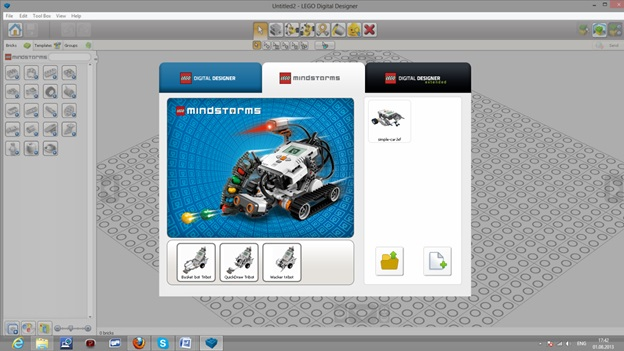
\includegraphics[width=0.76\linewidth]{chapters/chapter3/images/2}
		\caption{}
		\label{ris:image3x2}
	\end{center}
\end{figure}	

Кликнем по значку чистого листа (free build) в правом нижнем углу и создадим новый проект.
\begin{figure}[h!]
	\begin{center}
		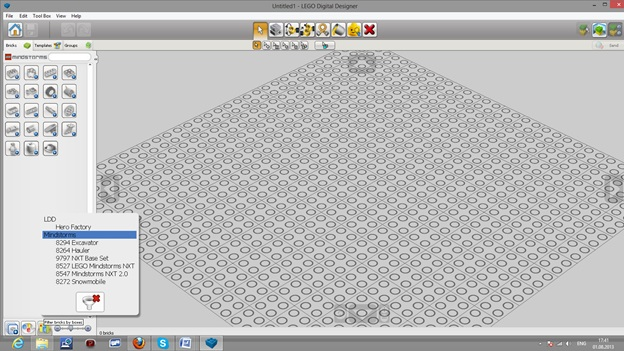
\includegraphics[width=0.8\linewidth]{chapters/chapter3/images/3}
		\caption{}
		\label{ris:image3x3}
	\end{center}
\end{figure}

В левом нижнем углу, под списком деталей, выберем Filter bricks by box (желтый значок) и выберем имеющийся у нас набор.
\begin{figure}[h!]
	\begin{center}
		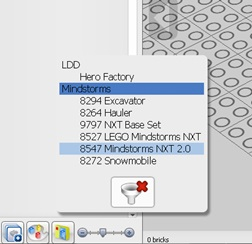
\includegraphics[width=0.65\linewidth]{chapters/chapter3/images/4}
		\caption{}
		\label{ris:image3x4}
	\end{center}
\end{figure}	

Количество доступных деталей уменьшиться, теперь их ровно столько же, сколько в нашем наборе.\\

{\hypertarget{lesson3x3}{\blackBlueText{IV. Модель совы}}}\\\\

{\bfseries Работа идет в режиме «наблюдай за мной, повторяй за мной». Преподаватель по шагам показывает, что нужно делать, выводя экран своего компьютера на проектор. После каждого шага учащимся предоставляется несколько минут, чтобы повторить действия преподавателя.}

\begin{enumerate}
	\item Сохраним файл. Для этого выбираем вкладку File->Save as \dots
	\begin{figure}[h!]
		\begin{center}
			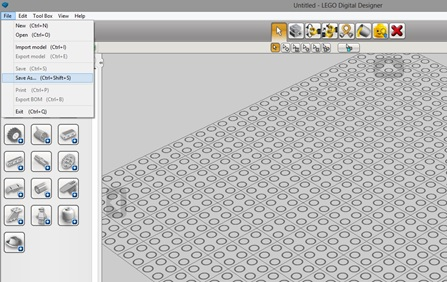
\includegraphics[width=1\linewidth]{chapters/chapter3/images/5}
			\caption{}
			\label{ris:image3x5}
		\end{center}
	\end{figure}
	\clearpage
	Выбираем папку, в которую хотим сохранить проект, и пишем его имя.
	\begin{figure}[h!]
		\begin{center}
			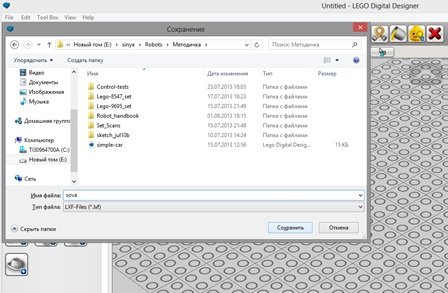
\includegraphics[width=1\linewidth]{chapters/chapter3/images/6}
			\caption{}
			\label{ris:image3x6}
		\end{center}
	\end{figure}
	Видим, что в заголовке имя тоже поменялось.
	\begin{figure}[h!]
		\begin{center}
			
\includegraphics[width=1\linewidth]{chapters/chapter3/images/7}
			\caption{}
			\label{ris:image3x7}
		\end{center}
	\end{figure}
	\clearpage
	\item Выбираем балку с 5 отверстиями.
	\begin{figure}[h!]
		\begin{center}
			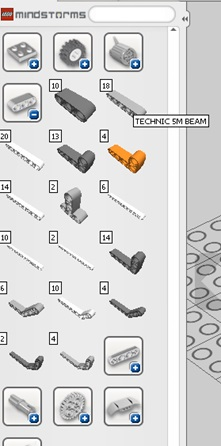
\includegraphics[width=0.7\linewidth]{chapters/chapter3/images/8}
			\caption{}
			\label{ris:image3x8}
		\end{center}
	\end{figure}
	Кладем ее на поле для сборки. По умолчанию она ложится горизонтально. С помощью стрелочек на клавиатуре поворачиваем ее на 90 градусов.
	\begin{figure}[h!]
		\begin{center}
			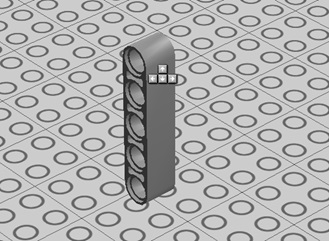
\includegraphics[width=0.79\linewidth]{chapters/chapter3/images/9}
			\caption{}
			\label{ris:image3x9}
		\end{center}
	\end{figure}
	\item Выбираем синий штифт и вставляем его в нижнее отверстие балки. Когда детали стыкуются, они подсвечиваются зеленой рамкой.
	\begin{figure}[h!]
		\begin{center}
			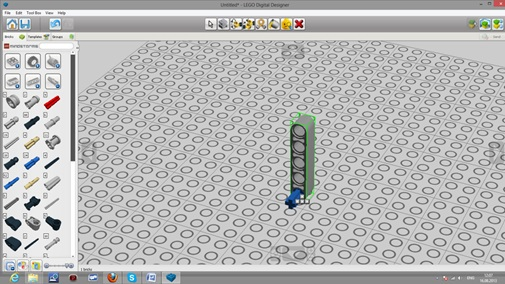
\includegraphics[width=1\linewidth]{chapters/chapter3/images/10}
			\caption{}
			\label{ris:image3x10}
		\end{center}
	\end{figure}
	\item Выбираем самую большую серую шестеренку и одеваем ее на штифт. В стандартном наборе нет серых шестеренок, есть аналогичная черная. Из эстетических соображений  в рассматриваемом примере сняты фильтры «by box» и собирается серая сова.
	\begin{figure}[h!]
		\begin{center}
			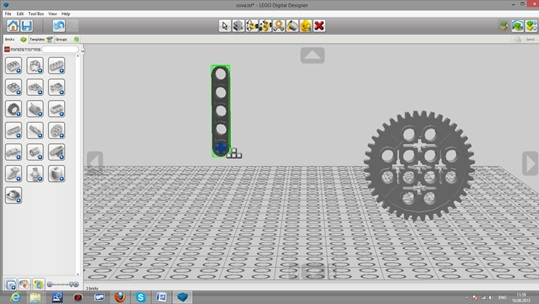
\includegraphics[width=1\linewidth]{chapters/chapter3/images/11}
			\caption{}
			\label{ris:image3x11}
		\end{center}
	\end{figure}
	\begin{figure}[h!]
		\begin{center}
			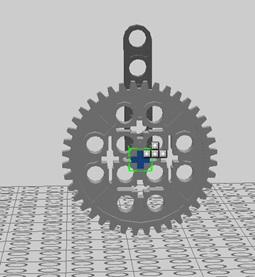
\includegraphics[width=0.55\linewidth]{chapters/chapter3/images/12}
			\caption{}
			\label{ris:image3x12}
		\end{center}
	\end{figure}
	\item Одеваем красный штифт и маленькую шестеренку.\\\\
	\begin{figure}[h!]
		\begin{center}
			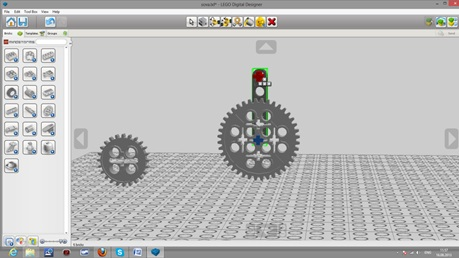
\includegraphics[width=1\linewidth]{chapters/chapter3/images/13}
			\caption{}
			\label{ris:image3x13}
		\end{center}
	\end{figure}
	\begin{figure}[h!]
		\begin{center}
			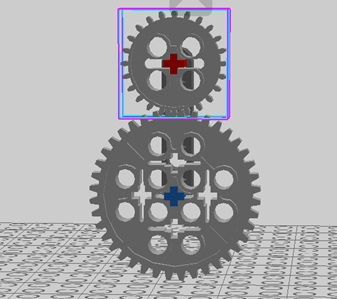
\includegraphics[width=0.67\linewidth]{chapters/chapter3/images/14}
			\caption{}
			\label{ris:image3x14}
		\end{center}
	\end{figure}
	При необходимости выбираем на верхней панели инструмент Hinge tool (H) и вращаем шестеренку, до зацепления зубцами.
	\item Укрепляем конструкцию еще одним синим штифтом. Добавляем ось со втулкой.
	\begin{figure}[h!]
		\begin{center}
			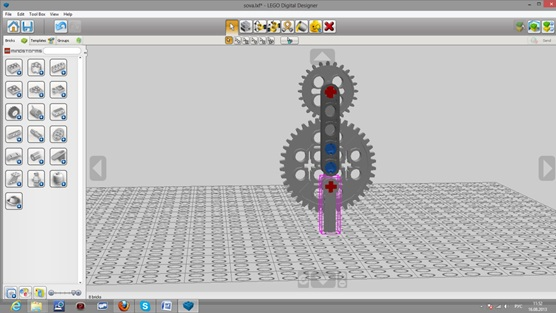
\includegraphics[width=1\linewidth]{chapters/chapter3/images/15}
			\caption{}
			\label{ris:image3x15}
		\end{center}
	\end{figure}
	\item Надеваем на ось балку с тремя отверстиями.
	\begin{figure}[h!]
		\begin{center}
			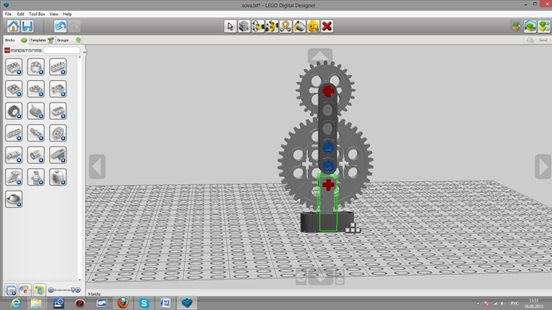
\includegraphics[width=1\linewidth]{chapters/chapter3/images/16}
			\caption{}
			\label{ris:image3x16}
		\end{center}
	\end{figure}
	\clearpage
	\item Добавляем черные штифты.
	\begin{figure}[h!]
		\begin{center}
			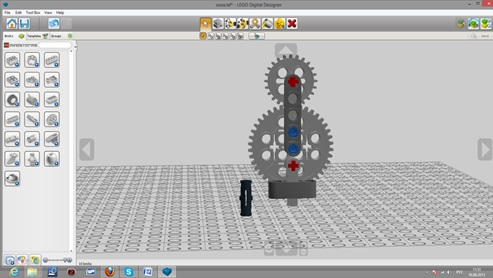
\includegraphics[width=1\linewidth]{chapters/chapter3/images/17}
			\caption{}
			\label{ris:image3x17}
		\end{center}
	\end{figure}
	\item Сажаем на пару черных штифтов крылья.
	\begin{figure}[h!]
		\begin{center}
			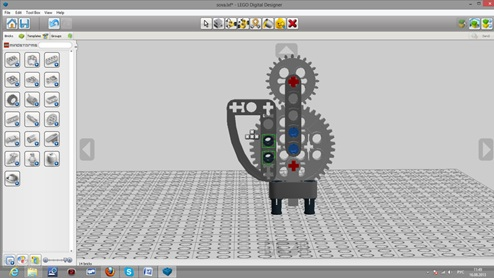
\includegraphics[width=1\linewidth]{chapters/chapter3/images/18}
			\caption{}
			\label{ris:image3x18}
		\end{center}
	\end{figure}
	\clearpage
	\item Добавляем соединители~--- лапы.
	\begin{figure}[h!]
		\begin{center}
			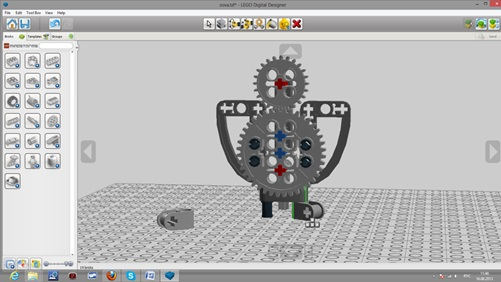
\includegraphics[width=1\linewidth]{chapters/chapter3/images/19}
			\caption{}
			\label{ris:image3x19}
		\end{center}
	\end{figure}
	\item Вставляем бежевые глаза.
	\begin{figure}[h!]
		\begin{center}
			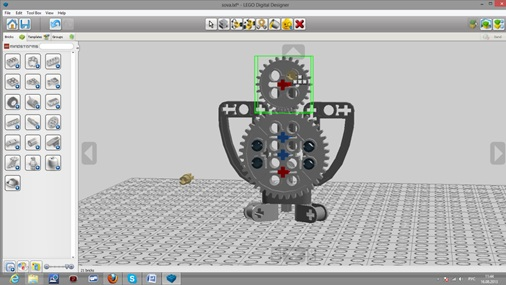
\includegraphics[width=1\linewidth]{chapters/chapter3/images/20}
			\caption{}
			\label{ris:image3x20}
		\end{center}
	\end{figure}
	\clearpage
	\item Сова готова!
	\begin{figure}[h!]
		\begin{center}
			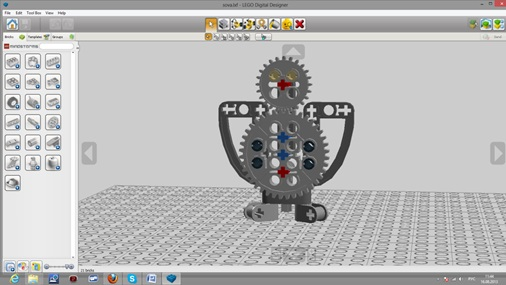
\includegraphics[width=1\linewidth]{chapters/chapter3/images/21}
			\caption{}
			\label{ris:image3x21}
		\end{center}
	\end{figure}
\end{enumerate}

{\slshape Можно дать детям немного свободного времени на усовершенствование совы~--- сделать ей клюв, уши, гнездо.}

В LDD есть очень полезная опция~--- Building guide mode, выбираемый в правом верхнем углу.
\begin{figure}[h!]
	\begin{center}
		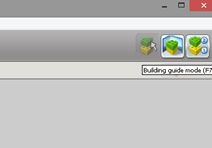
\includegraphics[width=0.75\linewidth]{chapters/chapter3/images/22}
		\caption{}
		\label{ris:image3x22}
	\end{center}
\end{figure}

В этом режиме программа по шагам можно проиграть, созданную программой инструкцию по сборке модели. Это бывает очень полезно при ознакомлении с чужой моделью и необходимости ее воспроизводства.
\begin{figure}[h!]
	\begin{center}
		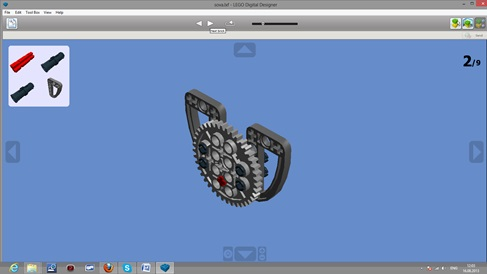
\includegraphics[width=1\linewidth]{chapters/chapter3/images/23}
		\caption{}
		\label{ris:image3x23}
	\end{center}
\end{figure}

Теперь предложите детям взять наборы и собрать сову в реальности, исполняя те шаги, которые предложит компьютер.
	\chapter{Простейшая трехколесная тележка}
{\bfseries Анонс:}\\\\
Работа с блоком NXT и сервомоторами без компьютера. Использование разных элементов питания, заряд батареи на экране. Простейшая трехколесная тележка. Подача напряжений на моторы.
{\bfseries Цели:}
\begin{itemize}
	\item{}{\bfseries Обучающие:} Закрепить  основы работы в Lego Digital Designer. Ознакомить с основными типами элементов питания и их особенностями. Обучить программированию на блоке NXT.  
	\item{}{\bfseries Развивающие:} Сформировать умение прослеживать причинно-следственные связи.\\
\end{itemize}	
{\bfseries Ход занятия:}\\\\
\begin{tabular}{lll}
	\hyperlink{lesson4x1}{1. Организационный момент} & Презентация & (5 мин)\\
	\hyperlink{lesson4x2}{2. Батареи блока NXT} & Презентация & (20 мин) \\
	\hyperlink{lesson4x3}{3. Управление моторами} & Практика & (30 мин) \\
	\hyperlink{lesson4x4}{4. Простейшая трехколесная} тележка & Практика & (55 мин)\\
\end{tabular}\\\\

{\hypertarget{lesson4x1}{\blackBlueText{I.Организационный момент}}}\\\\

Первая часть сегодняшнего занятия посвящена работе с аккумуляторами и простейшему программированию блока NXT.Эта работа может выполняться фронтально, за партами.

Вторая часть занятия подразумевает самостоятельную работу в парах или по одиночке со свободным доступам к компьютерам, с установленным Lego Digital Designer и сохраненным на Рабочем столе файлом simple-car.lxf , и столам для конструирования.\\\\

{\hypertarget{lesson4x2}{\blackBlueText{II. Батареи блока NXT}}}\\\\

Несмотря на то, что чаще всего программа для робота сначала создается и редактируется на компьютере, а затем компилируется и загружается в память блока NXT, некоторые задачи можно решить, даже когда компьютера нет под рукой. 

Оговорим некоторые используемые ниже термины. {\bfseries Батарея}~--- это электрический компонент, обеспечивающий питание одного блока NXT. Батарея может состоять из нескольких элементов. {\bfseries Батарейка}~--- пальчиковый элемент питания не пригодный для перезарядки. {\bfseries Аккумулятор}~--- пальчиковый многократно перезаряжаемый элемент питания. 

Как уже говорилось, в качестве элементов питания можно использовать как фирменный аккумулятор Lego, так и пальчиковые аккумуляторы и батарейки размера АА.\\\\
\greenText{Картинка с вопросом}\\\\

Рассмотрим главные различия между последними двумя источниками, а также в процессе отметим основные отличия от фирменного блока питания. Большое преимущество аккумуляторов перед батарейками заключается в том, что разряженные аккумуляторы можно зарядить и снова ими пользоваться. Поэтому, несмотря на то, что аккумуляторы, как правило, дороже батареек (разница в цене примерно на порядок, а к этому нужно еще прибавить стоимость зарядного устройства), экономически их долгосрочное использование оказывается выгоднее. При этом только важно приобрести хорошее и качественное зарядное устройство, которое будет «лечить» аккумуляторы при каждом процессе заряда, не позволяя их емкости уменьшаться.

Что такое емкость аккумулятора? Фактически эта величина характеризует запас энергии, которую способен запасти аккумулятор, а потом в процессе работы ее отдать. Чем больше емкость, тем больше энергии запасает аккумулятор и тем дольше он будет ее отдавать~--- то есть дольше работать. Измеряется емкость в мАч (миллиампер*часы)~--- то есть, по сути, произведение тока на время его протекания. Так как батарейки или аккумуляторы соединяют последовательно (а при последовательном соединении ток во всех элементах цепи, как известно, один и тот же), то емкость батареи из последовательно соединенных элементов равна емкости одного элемента. Емкости современных батареек колеблются от 1500 до 3100 мАч, аккумуляторов от 1500 до 2700 мАч. Разумеется, имеет смысл приобретать элементы питания с наибольшей емкостью. Для сравнения, фирменный блок питания Lego (9693) имеет емкость 2100 мАч, проигрывая, таким образом, батарейкам и аккумуляторам большой емкости.

Кроме емкости есть еще один важный параметр~--- напряжение. Эта величина в нашем случае влияет на то, с какой скоростью аккумулятор будет отдавать накопленную у него энергию, то есть какую максимальную силу сможет развить робот в данные момент времени, или с какой максимальной скоростью он сможет двигаться. Если проводить сравнение с физиологией человека, то емкость~--- это выносливость (как долго человек будет справляться с нагрузкой), а напряжение~--- это мгновенная сила (может ли спортсмен сделать рывок, или поднять большой вес). Если несколько элементов питания соединить последовательно, то их напряжения складываются. Итак, напряжение одного стандартного аккумулятора 1,2 В, напряжение одной стандартной батарейки 1,5 В. Так как для питания блока NXT используется 6 элементов, то батарея из 6 аккумуляторов будет иметь напряжение 7,2 В, а батарея из 6 батареек – 9 В. Для сравнения, фирменный блок питания Lego (9693) имеет напряжение 7,4 В. В данном сравнении аккумуляторы значительно проигрывают батарейкам. Если посчитать аккуратно, то выдаваемая мощность батареек выше на 56 \%. 

Итак, какие выводы можно сделать на основе изложенных фактов?

{\slshape К этому моменту дети уже начинают терять внимание, поэтому прежде чем приступить к важным для нас выводам разумно выслушать их предположения, еще раз подчеркнуть какие-то моменты и вместе придти к следующему:}

{\bfseries Аккумуляторы выносливее батареек, но проигрывают им по мгновенной мощности.} Фирменная батарея Lego находится где-то посередине. В данной ситуации для повседневной работы выгодным является использование аккумуляторов,  батарейки же могут понадобиться в случаях, когда необходима большая мгновенная мощность – например, на соревнованиях.

{\slshape Еще один момент, который полезно знать, касается установки аккумуляторов. Внутри аккумуляторного отсека блока NXT есть небольшая черная кнопочка.}\\\\
\greenText{фото}\\\\

{\slshape При установке фирменного блока питания Lego эта кнопочка оказывается нажатой. Нажатие влияет на то, как блок NXT оценивает заряд блока аккумуляторов. Для правильной оценки кнопочка должна быть нажата. Таким образом, в некоторых ситуациях блок NXT неправильно отображает оставшийся заряд вставленных пальчиковых аккумуляторов или батареек. Блок NXT отображает значок состояния батареи в верхнем правом углу экрана.}\\\\
\greenText{Фото заряда батареи}\\\\

Рассмотрим теперь, на что влияет состояние батареи. Самое главное, и, пожалуй, единственное – на мгновенную мощность моторов (как следствие, на максимальную скорость их вращения). Не влияет на показания счетчиков оборотов моторов. Так как все датчики питаются стабилизированным напряжением 5 В, их показания также не зависят от состояния батареи.
Интересный момент: блок NXT перестает включаться, если напряжение батареи ниже 5 вольт.

По мнению автора, на момент издания настоящего пособия, оптимальным решением вопроса выбора элементов питания являются аккумуляторы GP NiMn R06 (AA) 2700 mAh в совокупности с зарядным устройством Ansmann ENERGY 16 (PLUS).

После того, как мы разобрались с питанием для блока NXT, мы можем наконец-то его включить.\\\\

{\hypertarget{lesson4x3}{\blackBlueText{III. Управление моторами}}}\\\\	

При включении блока NXT открывается главное меню на вкладке My Files. Нажав центральную оранжевую кнопку попадаем в раздел, где хранятся программы, загруженные с компьютера (Software files)  и написанные на NXT (NXT files). Кроме них там содержится папка Sound files, в которую автоматически сохраняются звуковые файлы из загруженных программ. Переходить между папками можно при помощи серых стрелок.\\\\
\greenText{рис}\\\\

Сегодня мы научимся писать простейшие программы на самом блоке. Для этого в главном меню переходим с вкладки My Files на вкладку NXT Program. Любая программа на NXT состоит из 5 блоков.\\\\
\greenText{Описание и пример программы.}\\\\

{\hypertarget{lesson4x4}{\blackBlueText{IV. Простейшая трехколесная тележка}}}\\\\	

Теперь соберем простейшую трехколесную тележку и запрограммируем ее на движение вперед. В качестве инструкции по сборке детям предлагается модель тележки, созданная в LDD. 

Что бы открыть файл выберем File\(\to\)Open. В появившемся окне выбираем путь, ведущий к искомому файлу.
\clearpage
\begin{figure}[h!]
	\begin{center}
		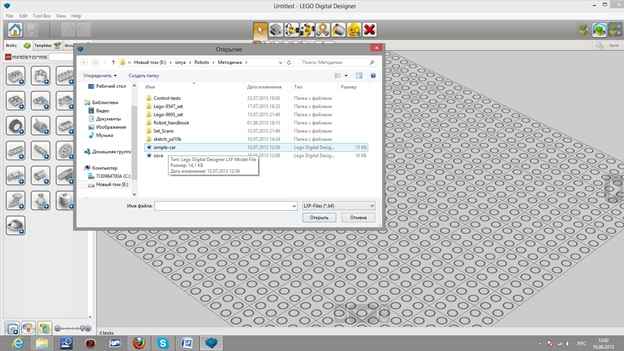
\includegraphics[width=0.95\linewidth]{chapters/chapter4/images/1}
		\caption{}
		\label{ris:image4x1}
	\end{center}
\end{figure}	 

Нажимаем «Открыть». Появляется модель тележки. Далее у детей есть свободное время (около 30 минут) на то, что бы собрать тележку в реальности. Методы которыми они при этом будут пользоваться не регламентированы~--- могу войти в режим «build guide», могут разбирать тележку по частым, могут просто крутить и приближать модель.

\begin{figure}[h!]
	\begin{center}
		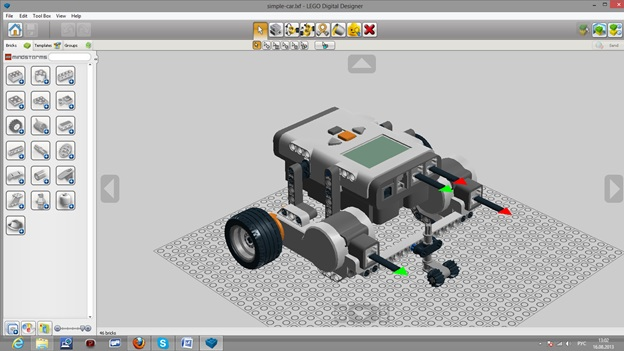
\includegraphics[width=0.95\linewidth]{chapters/chapter4/images/2}
		\caption{}
		\label{ris:image4x2}
	\end{center}
\end{figure}	

Итоговую тележку надо запрограммировать на блоке на движение прямо, как обсуждалось выше. Первый робот поехал!
	\chapter{Движение по окружности. Передачи.}
{\bfseries Анонс:}\\\\
Характеристики движения по окружности: скорость, период, частота, угловая скорость. Виды передач: фрикционная, ременная, зубчатая, червячная.\\\\
{\bfseries Цели:}
\begin{itemize}
	\item{}{\bfseries Обучающие:} Познакомить с основными понятиями кинематики криволинейного движения. Сформировать у учащихся представления об основных видах механических передач.
	\item{}{\bfseries Развивающие:}Формирование умений сравнивать, классифицировать, обобщать изучаемые факты и понятия. Развитие познавательного интереса для учащихся.\\
\end{itemize}	
{\bfseries Ход занятия:}\\\\
\begin{tabular}{lll}
	\hyperlink{lesson5x1}{1. Организационный момент} & Презентация & (5 мин)\\
	\hyperlink{lesson5x2}{2. Характеристики движения} & Презентация & (50 мин) \\
	\hyperlink{lesson5x3}{3. Виды передач} & Презентация & (20 мин) \\
	\hyperlink{lesson5x4}{4. Решение задач} & Практика & (30 мин)\\
\end{tabular}\\\\

{\hypertarget{lesson5x1}{\blackBlueText{I.Организационный момент}}}\\\\

В первой половине занятия предполагается запись теории и решение задач, поэтому следует заранее предупредить учащихся о необходимости принести тетради/блокноты. Рассказ по видам механических передач рекомендуется дополнять демонстрациями этих передач на макетах и видео.

Во второй части занятия следует решить несколько задач на характеристики движения по окружности.\\\\

{\hypertarget{lesson5x2}{\blackBlueText{II. Характеристики движения}}}\\\\

{\slshape Курс рассчитан на учащихся 8-ого класса и старше, так что при дальнейшем изложении материала предполагаются известными характеристики путь и скорость.} 

При движении тела по окружности (вращении)  зачастую оказывается удобно говорить не о пути s, пройденным телом, а об угле поворота \(\phi\). Угол \(\phi\) принято измерять не в градусах, а в специальных единицах радианах (рад). По определению радиана:
\begin{equation}
\phi=\frac{s}{r}
\end{equation}
\begin{figure}[h!]
	\begin{center}
		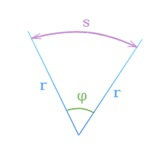
\includegraphics[width=0.27\linewidth]{chapters/chapter5/images/1}
		\caption{}
		\label{ris:image5x0x1}
	\end{center}
\end{figure}

Тогда получается, что вся окружность имеет угловую меру:
\begin{equation}
\phi=\frac{s}{r}=\frac{2\pi r}{r}=2\pi\mbox{ \slshape рад}
\end{equation}

С другой стороны, вся окружность имеет градусную меру \(360^{\circ}\). Таким образом, получаем формулу для перевода градусов в радианы и наоборот:
\begin{equation}
\frac{\phi_{\mbox{ \slshape рад}}}{\phi^{\circ}}=\frac{\pi}{180^{\circ}}
\end{equation}

Время одного полного оборота называют периодом и обозначают буквой \(T\). Величина, обратная периоду носит название частота, и обозначается буквой \(\nu\). Частота измеряется в герцах (Гц) и имеет смысл числа оборотов за единицу времени.
\begin{equation}
[T]=\mbox{\slshape c}
\end{equation} 
\begin{equation}
[\nu]=\frac{1}{\mbox{\slshape c}}=\mbox{\slshape Гц}
\end{equation}  
\begin{equation}
{T=\frac{1}{\nu}}
\end{equation}

При движении по окружности различают линейную и угловую скорости. Линейная скорость \(V\)~--- это путь \(\Delta s\), проходимый за единицу времени, так сказать «обычная» скорость. Угловой скоростью \(\omega\) называют угол \(\Delta\phi\), на который повернулось тело за единицу времени. Легко вывести формулу, связывающую линейную и угловую скорости.
\begin{equation}
V=\frac{\Delta s}{\Delta t}
\end{equation}
\begin{equation}
\omega=\frac{\Delta\phi}{\Delta t}
\end{equation} 
\begin{equation}
V=\frac{\Delta s}{\Delta t}=\frac{\Delta (\phi r)}{\Delta t}=\frac{r\Delta\phi}{\Delta t}=\omega r
\end{equation} 

За один полный оборот тело поворачивается на угол \(2\pi\) радиан, затрачивая на это время равное периоду \(T\). Тогда угловая скорость:
\begin{equation}
\omega=\frac{2\pi}{T}=2\pi\nu
\end{equation}\\\\

{\hypertarget{lesson5x3}{\blackBlueText{III. Виды передач}}}\\\\

При построении сложных механизмов часто возникает необходимость передавать вращение от мотора к другим частям конструкции. Для этого применяют различные виды передач: фрикционные, зубчатые, ременные, цепные и червячные.
\begin{figure}[h!]
	\begin{center}
		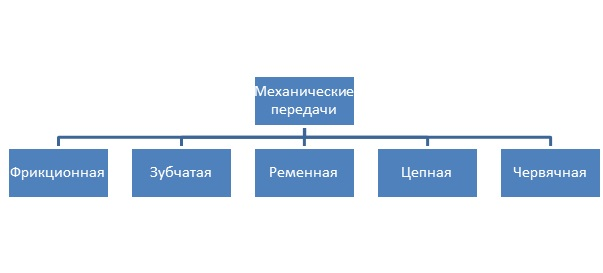
\includegraphics[width=0.9\linewidth]{chapters/chapter5/images/2}
		\caption{}
		\label{ris:image5x1}
	\end{center}
\end{figure}

При {\bfseries фрикционной} передаче вращение от одного колеса к другому передается при помощи силы трения. Оба колеса прижимаются друг к другу с некоторой силой и вследствие возникающего между ними трения вращают одно другое.\\
Достоинства фрикционной передачи:

\begin{itemize}
	\item Простота изготовления тел качения;	
	\item Равномерность вращения и бесшумность работы;
	\item Возможность включения/выключения передачи на ходу.\\
\end{itemize}
Недостатки фрикционной передачи:

\begin{itemize}
	\item Проскальзывание, ведущее к непостоянству передаточного числа и потери энергии;
	
	\item Необходимость обеспечения прижима.\\\\
\end{itemize}
\begin{figure}[h!]
	\begin{center}
		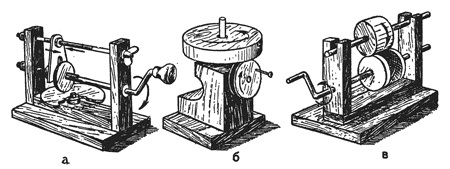
\includegraphics[width=1\linewidth]{chapters/chapter5/images/3}
		\caption{а~--- лобовая передача, б~--- угловая передача, в~--- цилиндрическая передача.}
		\label{ris:image5x2}
	\end{center}
\end{figure}
\clearpage
\begin{figure}[h!]
	\begin{center}
		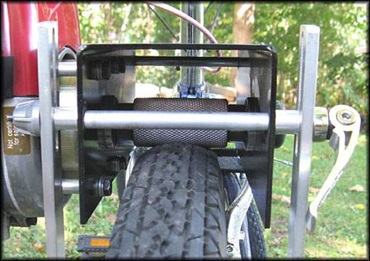
\includegraphics[width=1\linewidth]{chapters/chapter5/images/4}
		\caption{}
		\label{ris:image5x3}
	\end{center}
\end{figure}
\clearpage
В {\bfseries зубчатых} передачах вращение от одного колеса к другому передается при помощи зубьев. Зубчатые колеса вращаются намного легче фрикционных. Объясняется это тем, что здесь нажима колеса на колесо совсем не требуется. Для правильного зацепления и легкой работы колес профиль зубца делают по определенной кривой, называемой эвольвентой.
\begin{figure}[h!]
	\begin{center}
		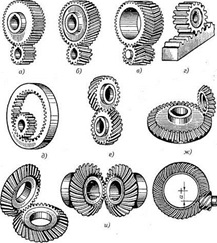
\includegraphics[width=1\linewidth]{chapters/chapter5/images/5}
		\caption{}
		\label{ris:image5x4}
	\end{center}
\end{figure}
\clearpage
\begin{figure}[h!]
	\begin{center}
		\includegraphics[width=1\linewidth]{chapters/chapter5/images/6}
		\caption{}
		\label{ris:image5x5}
	\end{center}
\end{figure}
Достоинства зубчатой передачи:

\begin{itemize}
	\item Значительно меньшие габариты, чем у других передач;	
	\item Высокий кпд (потери в точных, хорошо смазываемых передачах 1--2\%);	
	\item Большая долговечность и надёжность.\\
\end{itemize}
Недостатки зубчатой передачи:

\begin{itemize}
	\item Шум при работе;	
	\item Необходимость точного изготовления.\\
\end{itemize}

{\bfseries Ременная} передача, как и зубчатая, встречается очень часто. Ремень, натянутый на шкивы, охватывает какую-то их часть. Эта облегающая часть (дуга) носит, название угла обхвата. Чем больше будет угол обхвата, тем лучше образуется сцепление, лучше и надежнее будет вращение шкивов. При малом угле обхвата может получиться так, что ремень на малом шкиве станет проскальзывать, вращение будет передаваться плохо или его совсем не будет. Угол обхвата зависит от соотношения размеров шкивов и их расстояния друг от друга.

\begin{figure}[h!]
	\begin{center}
		\includegraphics[width=0.55\linewidth]{chapters/chapter5/images/7}
		\caption{Схемы ременчатых передач.}
		\label{ris:image5x6}
	\end{center}
\end{figure}
\begin{figure}[h!]
	\begin{center}
		\includegraphics[width=0.55\linewidth]{chapters/chapter5/images/8}
		\caption{Схемы ременчатых передач.}
		\label{ris:image5x7}
	\end{center}
\end{figure}
\clearpage
\noindent Достоинства ременной передачи:	

\begin{itemize}
	\item Простота конструкции;
	\item Возможность расположения ведущего и ведомого шкивов на больших расстояниях (более 15 метров);
	\item Плавность и бесшумность работы;
	\item Предохранение механизмов от перегрузки за счёт упругих свойств ремня и его способности проскальзывать по шкивам;
	\item Возможность работы с большими угловыми скоростями.\\
\end{itemize}
\noindent Недостатки ременной передачи:

\begin{itemize}
	\item Постепенное вытягивание ремней, их недолговечность (при больших скоростях работает от 1000 до 5000 часов);
	\item Непостоянство передаточного отношения (из-за неизбежного проскальзывания ремня);
	\item Относительно большие размеры.\\
\end{itemize}

{\bfseries Цепная} передача по сравнению с ременной удобна тем, что не дает проскальзывания и позволяет соблюдать правильность передаточного числа. Цепная передача осуществляется только при параллельных валах.

\begin{figure}[h!]
	\begin{center}
		\includegraphics[width=1\linewidth]{chapters/chapter5/images/9}
		\caption{}
		\label{ris:image5x8}
	\end{center}
\end{figure}	
\clearpage
\begin{figure}[h!]
	\begin{center}
		\includegraphics[width=0.72\linewidth]{chapters/chapter5/images/10}
		\caption{}
		\label{ris:image5x9}
	\end{center}
\end{figure}	
\noindent Достоинства цепной передачи:	

\begin{itemize}
	\item Меньшая чувствительность к неточностям расположения валов;
	\item Возможность передачи движения одной цепью нескольким звездочкам;
	\item Возможность передачи вращательного движения на большие расстояния.\\
\end{itemize}
Недостатки цепной передачи:

\begin{itemize}
	\item Повышенный шум и износ цепи при неправильном выборе конструкции, небрежном монтаже и плохом уходе.\\
\end{itemize}

{\bfseries Червячная} передача служит для получения вращения между валами, пересекающимися в одной плоскости. Передача состоит из винта (червяка) и винтового колеса, которые находятся в зацеплении. При вращении червяка витки ведут зубцы колеса и заставляют его вращаться. Обычно вращение от червяка передается колесу. Обратная передача почти не встречается из-за самоторможения.

\begin{figure}[h!]
	\begin{center}
		\includegraphics[width=0.8\linewidth]{chapters/chapter5/images/11}
		\caption{}
		\label{ris:image5x10}
	\end{center}
\end{figure}
\clearpage
\begin{figure}[h!]
	\begin{center}
		\includegraphics[width=0.90\linewidth]{chapters/chapter5/images/12}
		\caption{Схемы ременчатых передач.}
		\label{ris:image5x11}
	\end{center}
\end{figure}	
\noindent Достоинства червячной передачи:	

\begin{itemize}
	\item Плавность и бесшумность работы;
	\item Большое передаточное число;
	\item Передача вращения только в одном направлении.\\
\end{itemize}
Недостатки червячной передачи:

\begin{itemize}
	\item Усиленное тепловыделение;
	\item Повышенный износ;
	\item Склонность к заеданию;
	\item Сравнительно низкий кпд.\\\\
\end{itemize}

{\hypertarget{lesson5x4}{\blackBlueText{IV. Решение задач}}}\\\\

Теоретический материал из предыдущих пунктов рекомендуется дополнить решением задач. Часть из них может быть разобрана в классе, часть дана для самостоятельного изучения.

В зависимости от конкретной ситуации, учащихся можно вызывать на задачу «змейкой», каждый делает ровно одно действие; либо можно устроить небольшой турнир по задачам или «свою игру», с «котом в мешке» (например, построить реальную фрикционную передачу из стирательных резинок) и «вопросом-аукцион».\\\\

\newcounter{tasks}
\begin{itemize}
	\renewcommand{\labelitemi}{\stepcounter{tasks}\Roman{tasks}.}
	%\renewcommand{\theenumi}{\Roman{enumi}}
	\item Частота обращения ветроколеса ветродвигателя 30 об/мин, якоря электродвигателя 1500 об/мин, барабана сепаратора 8400 об/мин, шпинделя шлифовального станка 96 000 об/мин. Вычислить их периоды.
	\item Скорость точек рабочей поверхности наждачного круга диаметром 300 мм не должна превышать 35 м/с. Допустима ли посадка круга на вал электродвигателя, совершающего 1400 об/мин; 2800 об/мин?
	\item Частота обращения воздушного винта самолета 1500 об/мин. Сколько оборотов делает винт на пути 90 км при скорости полета 180 км/ч?
	\item Период обращения платформы карусельного станка 4 с. Найти скорость крайних точек платформы, удаленных от оси вращения на 2 м.
	\item Диаметр передних колес трактора в 2 раза меньше, чем задних. Сравнить частоты обращения колес при движении трактора.
	\item Радиус рукоятки колодезного ворота в 3 раза больше радиуса вала, на который наматывается трос. Какова линейная скорость конца рукоятки при поднятии ведра с глубины 10 м за 20 с?
	\item При увеличении в 4 раза радиуса круговой орбиты искусственного спутника Земли период его обращения увеличивается в 8 раз. Во сколько раз изменяется скорость движения спутника по орбите?	
	\item Минутная стрелка часов в 3 раза длиннее секундной. Найти отношение скоростей концов стрелок.\\
\end{itemize}
	\chapter{\label{lesson6}Передаточное соотношение}
{\bfseries Анонс:}\\\\
Передаточное соотношение. Соотношение на скорость. Соотношение на мощность. Запускающий механизм для волчка.\\\\
{\bfseries Цели:}
\begin{itemize}
	\item{}{\bfseries Обучающие:} Закрепить понятия угловая и линейная скорости, частота, период. Познакомить учащихся с понятием передаточного соотношения и видами передач.
	\item{}{\bfseries Развивающие:} Формирование умений сравнивать, классифицировать, обобщать изучаемые факты и понятия. Развитие познавательного интереса для учащихся.\\
\end{itemize}	
{\bfseries Ход занятия:}\\\\
\begin{tabular}{lll}
	\hyperlink{lesson6x1}{1. Организационный момент} & Презентация & (5 мин)\\
	\hyperlink{lesson6x2}{2. Движение по окружности} & Практика & (5 мин) \\
	\hyperlink{lesson6x3}{3. Передаточное соотношение} & Презентация & (50 мин) \\
	\hyperlink{lesson6x4}{4. Решение задач} & Практика & (30 мин)\\
	\hyperlink{lesson6x5}{5. Запускающий механизм волчка} & Игра & (30 мин)
\end{tabular}\\\\

{\hypertarget{lesson6x1}{\blackBlueText{I.Организационный момент}}}\\\\

Для первой части сегодняшнего занятия понадобятся тетради с предыдущей теорией. Для практикума по запуску волчка у каждого должен быть отдельный набор и рабочий стол для сбора и тестирования конструкции.\\\\

{\hypertarget{lesson6x2}{\blackBlueText{II. Движение по окружности}}}\\\\	

В качестве легкой разминки предлагается ряд устных вопросов по предыдущему материалу:

\begin{enumerate}
	\item Минутная стрелка часов делает один полный оборот. Чему равен период обращения?
	\begin{enumerate}
		\item 60 c;
		\item 1/3600 с;
		\item 3600 с.
	\end{enumerate}
	\item Колесо велосипеда делает один оборот за 4 с. Определите частоту вращения.
	\begin{enumerate}
		\item 0,25 1/с;
		\item 4 1/с;
		\item 2 1/с.
	\end{enumerate}
	\item  Винт моторной лодки делает 25 оборотов за 1 с. Чем, равна угловая скорость винта?
	\begin{enumerate}
		\item 25 рад/с;
		\item  \(\pi\)/25 рад/с;
		\item 50\(\pi\)рад/с.
	\end{enumerate}
	\item Определите частоту вращения сверла электрической дрели, если его угловая скорость равна 400 \(\pi\).
	\begin{enumerate}
		\item 800 1/с;
		\item 400 \(\pi\)1/с;
		\item 200 1/с.
	\end{enumerate} 
\end{enumerate}

{\bfseries Ответы  на тест:} в; а; в; в.
\clearpage
{\hypertarget{lesson6x3}{\blackBlueText{III. Передаточное соотношение}}}\\\\

В любой передаче линейные скорости крайних точек шестеренок совпадают. Тогда угловые скорости связаны соотношением:
\begin{figure}[h!]
	\begin{center}
		\includegraphics[width=1\linewidth]{chapters/chapter6/images/1}
		\caption{}
		\label{ris:image6x1}
	\end{center}
\end{figure}	
\begin{equation}
V_1=V_2\Rightarrow\omega_1 r_1=\omega_2 r_2\Rightarrow\frac{\omega_1}{\omega_2}=\frac{r_2}{r_1}=\frac{n_2}{n_1}=\iota_{12}    
\end{equation}

Для зубчатых и цепных передач радиусы относятся как число зубцов \(n_2\) и \(n_1\) (под первой шестеренкой здесь и далее понимается ведущая, под второй – ведомая). Это отношение обычно обозначают как \(\iota_12\)  и называют {\bfseries передаточным соотношением}.
\begin{equation}
\mbox{\underline{Для любознательных:} Доказать, что }\frac{r_2}{r_1}=\frac{n_2}{n_1}  
\end{equation}

Видно, что если \(\iota_{12}>1\), то скорость вращения в результате передачи понижается, и передача называется {\bfseries понижающей}.

Если  \(\iota_{12}<1\), то скорость вращения в результате передачи повышается, и передача называется {\bfseries повышающей}.

Но если мы выиграли в скорости, то в чем-то должны были проиграть? Все верно, {\bfseries во сколько раз выигрываем в скорости, во столько раз проигрываем в силе.}\\\\
\greenText{Инфографика}\\\\

В случае сложных систем, в передаче может быть задействовано несколько шестеренок. Возможны следующие варианты их расположения: шестеренки укреплены на одном валу.
\clearpage
\begin{figure}[h!]
	\begin{center}
		\includegraphics[width=1\linewidth]{chapters/chapter6/images/2}
		\caption{}
		\label{ris:image6x2}
	\end{center}
\end{figure}	

Или несколько шестеренок подряд сцеплено друг с другом.
\begin{figure}[h!]
	\begin{center}
		\includegraphics[width=1\linewidth]{chapters/chapter6/images/3}
		\caption{}
		\label{ris:image6x3}
	\end{center}
\end{figure}	

В первом случае (рис.~\ref{ris:image6x2}) совпадают угловые скорости вращения шестеренок, а линейные скорости краев относятся как их радиусы (число зубьев):
\begin{equation}
\omega_1=\omega_2\Rightarrow\frac{V_1}{r_1}=\frac{V_2}{r_2}\Rightarrow\frac{V_1}{V_2}=\frac{r_1}{r_2}=\frac{n_2}{n_1}
\end{equation}
\begin{equation}
\iota_{12}=1
\end{equation}

Передаточное соотношение в данном случае равно единице.

Можно показать, что при расчете сложной системы из многих шестеренок, можно пользоваться следующим правилом:

{\bfseries Передаточное соотношение системы равно произведению передаточных соотношений элементов системы.}
\clearpage
\begin{figure}[h!]
	\begin{center}
		\includegraphics[width=1\linewidth]{chapters/chapter6/images/4}
		\caption{}
		\label{ris:image6x4}
	\end{center}
\end{figure}

\begin{equation}
\iota_{14}=\iota_{12}*\iota_{23}*\iota_{34}
\end{equation}

Отметим, что в данном примере \(\iota{23}=1\).

\underline{Для любознательных:} Доказать, правило (1). 

Применив это правило к системе, изображенной на \greenText{рис.~\ref{ris:image6x3}} получим:
\begin{equation}
\iota_{14}=\iota_{12}*\iota_{23}*\iota_{34}=\frac{n_1}{n_2}*\frac{n_2}{n_3}*\frac{n_3}{n_4}=\frac{n_1}{n_4}
\end{equation}

Получается «промежуточные» шестеренки здесь не играют никакой роли и могут быть любыми? Да, поэтому они носят название {\bfseries паразитные} шестеренки. Но, значит ли это, что такие шестеренки бессмысленны и подобные конструкции никогда не применяются? Нет, паразитные шестерни могут быть полезны как минимум в двух случаях:
\begin{itemize}
	\renewcommand{\textbullet}{\textendash}
	\item Передача вращения без изменения направления вращения. 
	\item Передача вращения на большое расстояние.\\\\
\end{itemize}

{\hypertarget{lesson6x4}{\blackBlueText{IV. Решение задач}}}\\\\

Теоретический материал из предыдущих пунктов рекомендуется дополнить решением задач. Часть из них может быть разобрана в классе, часть дана для самостоятельного изучения.
\begin{itemize}
	\renewcommand{\labelitemi}{\stepcounter{tasks}\Roman{tasks}.}
	\item Движение от шкива I (рис.~\ref{ris:image6x5}) к шкиву IV передается при помощи двух ременных передач. Найти частоту обращения (в об/мин) шкива IV, если шкив I делает 1200 об/мин, а радиусы шкивов r1 = 8 см, r2 = 32 см, r3 = 11 см, r4 = 55 см. Шкивы II и III жестко укреплены на одном валу.
	\clearpage
	\begin{figure}[h!]
		\begin{center}
			\includegraphics[width=0.8\linewidth]{chapters/chapter6/images/5}
			\caption{К задаче \Roman{tasks}.}
			\label{ris:image6x5}
		\end{center}
	\end{figure}
	\item Циркулярная пила имеет диаметр 600 мм. На ось пилы насажен шкив диаметром 300 мм, который приводится во вращение посредством ременной передачи от шкива диаметром 120 мм, насаженного на вал электродвигателя. Какова скорость зубьев пилы, если вал двигателя совершает 1200 об/мин?
	\item Диаметр колеса велосипеда «Пенза» d = 70 см, ведущая зубчатка имеет г1 = 48 зубцов, а ведомая z2 = 18 зубцов. С какой скоростью движется велосипедист на этом велосипеде при частоте вращения педалей п = 1 об/с? С какой скоростью движется велосипедист на складном велосипеде «Кама» при той же частоте вращения педалей, если у этого велосипеда соответственно d = 50 см, г1 = 48 зубцов, z2 = 15 зубцов?
\end{itemize}
\clearpage
{\hypertarget{lesson6x5}{\blackBlueText{V. Запускающий механизм волчка}}}\\\\

Для лучшего понимания понятий передаточное соотношение, повышающая передача предлагается провести следующее соревнование.

Каждому учащемуся предлагается собрать волчок из оси, насадив на нее колесо, как показано на рисунке.
\begin{figure}[h!]
	\begin{center}
		\includegraphics[width=0.8\linewidth]{chapters/chapter6/images/6}
		\caption{}
		\label{ris:image6x6}
	\end{center}
\end{figure}

Такой волчок можно легко запустить  рукой и он будет вращаться  10--20 секунд. Что нужно сделать, чтобы увеличить время вращения волчка? Ответ очевиден~--- изначально раскрутить его посильнее. Для этого мы сконструируем специальный механизм запускающий волчок.
\clearpage
\begin{figure}[h!]
	\begin{center}
		\includegraphics[width=0.9\linewidth]{chapters/chapter6/images/7}
		\caption{}
		\label{ris:image6x7}
	\end{center}
\end{figure}
\begin{figure}[h!]
	\begin{center}
		\includegraphics[width=0.9\linewidth]{chapters/chapter6/images/8}
		\caption{}
		\label{ris:image6x8}
	\end{center}
\end{figure}

Теперь пальцы раскручивают большую шестеренку, которая передает вращение маленькой, на оси волчка. У нас получилась повышающая передача с коэффициентом \greenText{столько-то}.

Теперь можно предложить детям собрать запускающие устройства с большим количеством шестеренок и устроить соревнования! Побеждает тот, чей волчок вращается дольше всего.

{\slshape Из набора 8547 можно собрать запускающее устройство с передаточным соотношением \greenText{столько-то}. Однако, для прокручивания первой шестеренки в таком случае нам надо приложить в \greenText{столько-то} же раз большую силу, а ведь есть еще и неучтенные нами потери на трение деталей друг о друга. Поэтому самый оптимальный с практической точки зрения механизм оказывается двухступенчатым:	
	\begin{figure}[h!]
		\begin{center}
			\includegraphics[width=1\linewidth]{chapters/chapter6/images/9}
			\caption{}
			\label{ris:image6x9}
		\end{center}
	\end{figure}
	
	Время вращения при этом доходит до \greenText{столько-то} секунд.}
	\chapter{Основные моменты устройства автомобиля}
{\bfseries Анонс:}\\\\
Самостоятельные доклады учащихся по различным узлам автомобиля.\\\\
{\bfseries Цели:}
\begin{itemize}
	\item{}{\bfseries Обучающие:} Раскрыть основные моменты устройства автомобиля: дифференциал, реечное рулевое управление, ручная и автоматические коробки передач.
	\item{}{\bfseries Развивающая:} Развивать умение извлекать знания из различных источников, речь учащихся, интерес к изучаемому предмету. Привить навыки самообразования.\\
\end{itemize}	
{\bfseries Ход занятия:}\\\\
\begin{tabular}{lll}
	\hyperlink{lesson7x1}{1. Реечное рулевое управление} & Презентация & (15 мин)\\
	\hyperlink{lesson7x2}{2. Дифференциал} & Презентация & (15 мин) \\
	\hyperlink{lesson7x3}{3. Ручная коробка передач} & Презентация & (15 мин) \\
	\hyperlink{lesson7x4}{4. Автоматическая коробка передач} & Презентация & (10 мин)\\
	\hyperlink{lesson7x5}{5. Принципы оформления презентаций} & Рефлексия & (20 мин)\\
	\hyperlink{lesson7x6}{6. Принципы публичных выступлений} & Рефлексия & (20 мин)\\
\end{tabular}\\\\

{\hypertarget{lesson7x1}{\hypertarget{lesson7x2}{\hypertarget{lesson7x3}{\hypertarget{lesson7x4}{\blackBlueText{I--IV. Реечное рулевое управление. Дифференциал. Ручная коробка передач.  Автоматическая коробка передач.}}}}}}\\\\

Темы докладов для учащихся подобраны таким образом, что бы повторить основные характеристики движения по окружности движение по окружности и зубчатых передач.  Непосредственно устройство дифференциала, рулевого управления и коробок передач в дальнейшем курсе использоваться не будут, литература по предмету широко доступна, поэтому данный урок не включает в себя материал по самим механическим системам. В принципы, темы могут быть скорректированы или заменены на другие по усмотрению преподавателя. Основная цель данного занятия (можно оформить его как мини конференцию с программками и докладчиками ) – повторить материал предыдущих занятий, показать тесную связь этой теории с реальными, окружающими детей механизмами и развить навыки публичных выступлений у учащихся.\\\\

{\hypertarget{lesson7x5}{\blackBlueText{V. Принципы оформления презентаций}}}\\\\

\begin{flushright}
	«Идеальная презентация~--- это десять слайдов тридцатым шрифтом».
\end{flushright}

Сегодня, редкое публичное выступление обходится без презентации. Презентации делают пятиклассники для уроков и академики для докладов. Самый простой и распространенный редактор Microsoft PowerPoint интуитивно осваивается за 20 минут и дает огромные возможности по формам представления информации. Тем не менее, очень многие докладчики, вне зависимости от возраста и статуса, совершают досадные ошибки в составлении презентаций, на которые хотелось бы обратить внимание.

Главное, что нужно осознать: презентация лишь дополняет вашу речь, основное внимание слушателей должно быть сосредоточено на докладе. В хорошей презентации нет больших объемов текста - их долго, неудобно читать и это отвлекает слушателя. В хорошей презентации нет дополнительной информации, не связанной с текстом доклада. В хорошей презентации нет выплывающих, выпрыгивающих, выцветающих блоков, если вы, конечно, презентуете не карнавальное агентство.

Что же есть в этой загадочной хорошей презентации? Титульный и финальный слайд. На титульном слайде положено представить название своей работы, автора, руководителя и учебное заведение/объединение. На финальном слайде поблагодарите слушателей за внимание. Единое деловое оформление всех слайдов. Схемы, блок-схемы, диаграммы, графики, рисунки. Смысл слайдов в том чтобы дать визуальный образ вашей речи, внутренних связей между предметами, причин и следствий.

Из вышесказанного очевидно, что докладчик ни в коем случае не должен читать свою презентацию. Расставляя смысловые акценты в своей речи, он иллюстрирует ключевые моменты на слайдах, стоя лицом к аудитории, а не к слайду.\\\\

{\hypertarget{lesson7x6}{\blackBlueText{VI. Принципы публичных выступлений}}}\\\\	

\begin{flushright}
	«Если вы не можете объяснить это просто - значит, вы сами не понимаете этого до конца»	
	
	А.Энштейн.
\end{flushright}

Ораторское мастерство – это целое искусство, которому посвящены тысячи томов, учебных курсов и тренингов. Не имея целью полно осветить все сложности этого искусства, хочется остановиться на нескольких наиболее простых и часто встречающихся проблемах учащихся. 

Главная проблема~--- это, конечно, полное не владение материалом доклада. К сожалению, отличная изначально идея рефератов и докладов учащихся сведена зачастую к «загуглил--скопировал--прочитал по бумажке-получил свою пять». Многие впервые начинают читать свой реферат уже на занятии.
Первое с чего нужно начать~--- это максимально мотивировать учащихся. Заинтересовать их темами доклада, поставить проблемные вопросы, добавить игровой момент («настоящая» конференция с докладчиками, трибуной, программой) и соревновательный (листы оценки и самооценки, поощрение за лучшее выступление). 

К сожалению, одной мотивации недостаточно, нужно уметь работать с текстом и готовиться выступать. Проверка «понимаю ли я то, о чем собираюсь говорить?» проста, нужно попробовать пересказать текст своими словами. Получилось? Теперь надо попробовать пересказать текст кому-то из знакомых или родственников, абсолютно не разбирающихся в вопросе. Достигнув понимания материала, следует так же проверить наличие у доклада внутренней структуры. Любое выступление имеет введение, заключение и основную часть, разбитую на логические блоки, взаимосвязанные между собой.

Итак, есть ответы на вопрос «что я хочу сказать?» и «как я хочу это сказать?». Но остается не менее сложная задача – действительно сказать это перед аудиторией. Даже самая логичная, структурированная и умная речь может быть озвучена так, что ничего не будет понятно.  Рекомендации будут очень просты, но отработке каждого пункта стоит уделить внимание.
\begin{itemize}
	\item Говорить надо громко. {\slshape Дайте каждому ребенку возможность громко что-то сказать.}
	\item Говорить надо с интонациями и паузами. {\slshape Прочитайте отрывок текста из любого доклада с интонациями и паузами, а не монотонной бубнежкой под нос. Потренируйте детей выделять основную мысль в предложении и интонировать ее.}
	\item Не надо спешить. Протараторьте и произнесите нарочито медленно. {\slshape Обсудите убыстряется или замедляется темп речи при публично выступлении. Проведите опыт.}
	\item Не надо бояться запнуться, остановиться или посмотреть в доклад. {\slshape Поясните разницу между читать доклад и подглядывать в план. Потренируйтесь преодолевать запинки и оговорки.} 
\end{itemize}
	\chapter{Соревнования  «Сумо»}
{\bfseries Анонс:}\\\\
Соревнования простейших сумоистов. Анализ проблем устойчивости конструкций. Сила трения, центр тяжести, устойчивость.\\\\
{\bfseries Цели:}
\begin{itemize}
	\item{}{\bfseries Обучающие:} Закрепить понятия передаточного соотношения. Улучшить навыки конструирования. Добиться формулировки и понимания основных законов равновесия и устойчивости конструкции.
	\item{}{\bfseries Развивающая:} Сформировать умение прослеживать причинно-следственные связи.\\
\end{itemize}	
{\bfseries Ход занятия:}\\\\
\begin{tabular}{lll}
	\hyperlink{lesson8x1}{1. Организационный момент} & Презентация & (5 мин)\\
	\hyperlink{lesson8x2}{2. Соревнования  «Сумо»} & Игра & (60 мин) \\
	\hyperlink{lesson8x3}{3. Проблемы устойчивости} & Рефлексия & (10 мин) \\
	\hyperlink{lesson8x4}{4. Центр тяжести} & Презентация & 40 мин)\\
\end{tabular}\\\\

{\hypertarget{lesson8x1}{\blackBlueText{I. Организационный момент}}}\\\\
\\\\

{\hypertarget{lesson8x2}{\blackBlueText{II. Соревнования «Сумо»}}}\\\\

Учащиеся делятся на команды по 2--3 человека. Каждой команде предлагается придумать свое название, все команды вносятся в турнирную таблицу (рисуется на доске или проецируется на экран с компьютера), по принципу каждый с каждым.

Каждая команда получает задание~--- за 20 минут собрать на основе стандартной тележки и придуманных понижающих передач робота, который перетолкает соперника.\\\\

{\bfseries Регламент состязаний:}
\begin{enumerate}
	\item Робот должен быть собран на основе стандартной трехколесной тележки, но допустимы надстройки на нее.
	\item Программа робота пишется на блоке, одинакова для всех участников и представляет собой: Forward\(\to\)Empty\(\to\)Forward\(\to\)Empty\(\to\)Loop.
	\item В стартовой позиции роботы стоят напротив друг друга на расстоянии 10 см.
	\item По команде «Старт» участники запускаю программу на своих роботов. После этого вмешиваться в работу роботов запрещено!
	\item \label{sumoVinner}Победа присуждается роботу, который протолкал своего соперника более 10 секунд подряд.
	\item Если роботы находятся в контакте и не двигаются более 15 секунд, присуждается ничья.
	\item За победу команда получает 2 очка, за ничью 1 очко, за проигрыш~--- 0 очков.
	\item После проведения отборочных матчей В полуфинал проходят 2 команды с наибольшим количеством очков.
\end{enumerate}

{\slshape При большом количестве команд разумно провести 2 полуфинала, финал и матч за третье место.
	
	Матчи можно проводить на специальном поле (см. Приложение), тогда пункт \ref{sumoVinner} может выглядеть таким образом:  Победа присуждается роботу, который вытолкал своего противника за пределы круга.}\\\\

{\hypertarget{lesson8x3}{\blackBlueText{III. Проблемы устойчивости}}}\\\\	

После соревнований проводится анализ технических решений, приводивших команды к успеху или проигрышу, причем ценен любой опыт.
\begin{enumerate}
	\item Использовали ли вы понижающую передачу?
	\item Каково было передаточное соотношение у вас? У ваших соперников? 
	\item Буксовал ли ваш робот? Как этого можно было избежать?
	\item Покажите ведущие колеса вашего робота? Где сосредоточена основная масса вашего робота?
	\item Легко ли переворачивается ваш робот? Как можно сделать робота устойчивее?
\end{enumerate}

{\hypertarget{lesson8x4}{\blackBlueText{IV.  Центр тяжести}}}\\\\

Можно заметить, что некоторые роботы буксовали, т.е.  мощность двигателя расходовалась впустую. Что бы такого не происходило, запомним важное правило: {\bfseries основной вес робота должен приходится на ведущие колеса}. Оказывается, что чем больше давление, оказываемое колесом, тем больше трение между колесом и поверхностью, а значит и сцепление с поверхностью.

Возможно, вы заметили, что некоторые роботы легко переворачивались. Попробуем сформулировать законы равновесия и выяснить, как собрать устойчивого робота. Поэкспериметируем с равновесием. Встанем прямо, ноги вместе и попробуем немного отклониться. Ой, падаем! Как бы встать поустойчивее? Достаточно расставить ноги чуть пошире, на ширину плеч.

Получается, чем шире основание, тем устойчивее предмет? На первый взгляд похоже на правду, пирамиду явно сложнее уронить, когда она стоит основанием, а не вершиной на земле.
\begin{figure}[h!]
	\begin{center}
		\includegraphics[width=0.35\linewidth]{chapters/chapter8/images/1}
		\caption{}
		\label{ris:image8x1}
	\end{center}
\end{figure}

Но маленький цилиндр явно устойчивее большого, хотя площади опоры у них и одинаковы. Получается дело не в опоре или не только в ней?
\begin{figure}[h!]
	\begin{center}
		\includegraphics[width=0.35\linewidth]{chapters/chapter8/images/2}
		\caption{}
		\label{ris:image8x2}
	\end{center}
\end{figure}

Проведем такой опыт: положим пустой коробок на стол, а в него положим  тяжелую гайку. Сдвинем ее как можно ближе к одному краю. Теперь этот край будет удерживаться на столе, даже если почти весь коробок висит в воздухе.
\begin{figure}[h!]
	\begin{center}
		\includegraphics[width=0.5\linewidth]{chapters/chapter8/images/3}
		\caption{}
		\label{ris:image8x3}
	\end{center}
\end{figure}

Т.е. если основная масса тела находится над опорой тело не упадет? Хорошая догадка, но как понять где сосредоточена «основная масса» однородного цилиндра? 

Оказывается, чтобы строго сформулировать закон равновесия необходимо ввести понятие центра тяжести. {\bfseries Центром тяжести} механической системы называется точка, относительно которой суммарный момент силы, действующих на систему, равен нулю. 

{\slshape Тут необходимо лирическое отступление. Формально, понятие момента силы могло звучать у детей на уроке физики еще в 7 классе, при изучении темы «Рычаги». Однако, опыт показывает, что разъяснение определение в таком виде, как оно дано выше,  восьми – и девятиклассникам требует глубокого отступления и напоминания понятий сила, момент силы, правила моментов и решения задач на статику. А главное, в курсе робототехнике это, в отличие от кинематики вращательного движения, подробно расписанной выше, не сильно пригодится. Достаточно будет понимания того, что не стоит задирать тяжелые блоки робота наверх конструкции. Поэтому дальнейший текст написан в расчете на то, что перед младшими можно помахать руками и сказать что-то туманное о «точке, около которой сосредоточена основная масса тела». Категорически неверно, но в тандеме с предлагаемыми опытами формирует понимание этого понятия «на пальцах».}

Центр тяжести шара находится в центре, цилиндра – на половине высоты, кольца – в центре кольца, т.е. центр тяжести не обязан находится внутри самого тела. Центр тяжести человека обычно расположен в районе живота.
\begin{figure}[h!]
	\begin{center}
		\includegraphics[width=1\linewidth]{chapters/chapter8/images/4}
		\caption{Центр масс человека}
		\label{ris:image8x4}
	\end{center}
\end{figure}	 

А искомый закон равновесия можно сформулировать так: {\bfseries перпендикуляр, опущенный из центра тяжести должен попадать в площадь опоры}. 
\begin{figure}[h!]
	\begin{center}
		\includegraphics[width=0.45\linewidth]{chapters/chapter8/images/5}
		\caption{}
		\label{ris:image8x5}
	\end{center}
\end{figure}

Применим этот закон, к нашим опытам. Человек будет стоять, не падая, до тех пор пока перпендикуляр опущенный из его центра масс не выйдет за площадь опоры. Понятно, что расставляя ноги шире мы увеличиваем площадь опоры и нас сложнее уронить.
\begin{figure}[h!]
	\begin{center}
		\includegraphics[width=0.75\linewidth]{chapters/chapter8/images/6}
		\caption{}
		\label{ris:image8x6}
	\end{center}
\end{figure}

У высокого цилиндра и центр тяжести оказывается выше. Таким образом его надо отклонить на меньший угол, что бы перпендикуляр, опущенный из центра масс вышел за площадь опоры. Это мы и подразумеваем под словом «устойчивее».
\begin{figure}[h!]
	\begin{center}
		\includegraphics[width=0.75\linewidth]{chapters/chapter8/images/7}
		\caption{}
		\label{ris:image8x7}
	\end{center}
\end{figure}

На самом деле, есть еще один случай, когда тело будет находится в состоянии устойчивого равновесия. Проведем следующий опыт. Попробуем поставить карандаш на острие. Не получается? Не удивительно, площадь опоры-то малюсенькая и при любом самом незначительном наклоне, перпендикуляр, опущенный из центра масс, выходит за площадь опоры.

Но есть один старинный фокус, как заставить карандаш стоять на острие. В него надо воткнуть перочинный нож, как показано на рисунке.
\begin{figure}[h!]
	\begin{center}
		\includegraphics[width=0.2\linewidth]{chapters/chapter8/images/8}
		\caption{}
		\label{ris:image8x8}
	\end{center}
\end{figure}

Минутку, а где же находится центр тяжести подобной системы? Очевидно, что нож тяжелее карандаша, так что центр тяжести находится где-то под пальцем, ПОД опорой. И мы можем сформулировать дополнение к нашему закону равновесия: {\bfseries равновесие будет устойчиво, если центр тяжести находится ниже точки опоры}.

Так что на канатных дорогах в горах можно кататься совершенно спокойно, ведь кабинка висит под тросом и главная тяжесть находится ниже точки опоры. На основе этого же закона в одном из технических музеев Финляндии есть аттракцион~--- велосипед, на котором каждый может проехаться по тросу  высоко над землей.
\begin{figure}[h!]
	\begin{center}
		\includegraphics[width=0.75\linewidth]{chapters/chapter8/images/9}
		\caption{}
		\label{ris:image8x9}
	\end{center}
\end{figure}

Упражнение для любознательных: Какой элемент представленной конструкции делает поездку безопасной?

Резюмируя наши знания об устойчивости и сцеплении с дорогой, можно дать две простые рекомендации по сборке любых ваших роботов. Основная масса должна быть всегда сосредоточена над ведущими колесами и как можно ниже!
	\chapter{Соревнования  «Гонки», RobotC}
{\bfseries Анонс:}\\\\
Соревнования «Гонки». Анализ технических решений. Проблемы командного взаимодействия. Языки программирования. Среда программирования RobotC. Общая структура программы.\\\\
{\bfseries Цели:}
\begin{itemize}
	\item{}{\bfseries Обучающие:} Повторение понятий передаточное соотношение, повышающая передача. Развитие навыков простейшего конструирования. Закрепление  принципов устойчивости конструкций. Знакомство с редактором RobotC.
	\item{}{\bfseries Коммуникативная:} Обучение детей работать во взаимодействии с другими учащимися (работа в группах) и учителем.\\
\end{itemize}	
{\bfseries Ход занятия:}\\\\
\begin{tabular}{lll}
	\hyperlink{lesson9x1}{1. Организационный момент} & Презентация & (5 мин)\\
	\hyperlink{lesson9x2}{2. Соревнования «Гонки»} & Игра & (50 мин) \\
	\hyperlink{lesson9x3}{3. Анализ технических решений} & Рефлексия & (15 мин) \\
	\hyperlink{lesson9x4}{4. Проблемы командного взаимодействия} & Рефлексия & 10 мин)\\
	\hyperlink{lesson9x5}{5. Языки программирования.Среда RobotC} & Презентация & 15 мин)\\
	\hyperlink{lesson9x6}{6. Практикум «Ленивая программа»} & Практика & 15 мин)\\
\end{tabular}\\\\

{\hypertarget{lesson9x1}{\blackBlueText{I. Организационный момент}}}\\\\ 

Первая часть занятия пройдет в режиме соревнований команд, каждой команде понадобиться свое рабочее место с набором и компьютером. Помимо этого следует выделить место под испытательный полигон, где дети смогут протестировать своих робот и засечь их результаты.

Во второй части занятия преподавателю потребуется проектор, а каждому учащемуся~--- компьютер с RobotC и блок NXT.\\\\

{\hypertarget{lesson9x2}{\blackBlueText{II.   Соревнования «Гонки» }}}\\\\

Учащиеся делятся на команды по 2--3 человека. Каждой команде предлагается придумать свое название, все команды вносятся в турнирную таблицу (рисуется на доске или проецируется на экран с компьютера).
Каждая команда получает задание~--- за 20 минут собрать гоночного робота, который быстрее всего преодолеет прямой участок трассы.\\\\
{\bfseries Регламент состязаний:}

\begin{enumerate}
	\item Программа робота пишется на блоке, одинакова для всех участников и представляет собой: Forward\(\to\)Empty\(\to\)Forward\(\to\)Empty\(\to\)Loop.
	\item По команде «Старт» участники запускаю программу на своих роботах. После этого вмешиваться в работу роботов любыми способами  запрещено!
	\item Роботы должны преодолеть ровный горизонтальный участок, протяженностью 10 метров.
	\item У каждой команды есть 3 попытки. В зачет идет лучший результат.
	\item Перерыв между попытками составляет не менее 5 минут.
	\item Победа присуждается роботу, показавшему лучшее время по результатам трех попыток.\\\\
\end{enumerate}

{\hypertarget{lesson9x3}{\blackBlueText{III. Анализ технических решений}}}\\\\

\begin{enumerate}
	\item Использовали ли вы повышающую передачу?
	\item Каково было передаточное соотношение?
	\item Покажите ведущие колеса вашего робота? Где сосредоточена основная масса вашего робота?
	\item Почему вы думаете, робот ехал не совсем прямо?*
	\item Как можно добиться прямолинейного движения?*
\end{enumerate}

{\slshape *Эти вопросы, касающиеся разных условий движения и управления правого и левого колеса, рекомендуется обсуждать только в сильных группах. Поиск путей решения проблемы подводит детей к идеи подчинения ( синхронизации) моторов, которую можно подробнее обсудить уже при изучении команды syncMotor.}\\\\

{\hypertarget{lesson9x4}{\blackBlueText{IV. Проблемы командного взаимодействия}}}\\\\

\begin{enumerate}
	\item Как вы выбрали, чью модель гоночной машины реализовывать?
	\item Изучили ли вы оба решения прежде, чем выбрать? Было ли ваше итоговое решение комбинацией изначальных? Или вы придумали новое, оптимальное?
	\item Сложно ли было договориться друг с другом?
	\item Услышал ли ваши предложения ваш напарник?
	\item Как вы распределили обязанности в процессе построения робота?
	\item Изменяли ли вы конструкцию вашего робота в перерывах между попытками? Как вы договаривались, что стоит изменить?\\\\
\end{enumerate}

{\hypertarget{lesson9x5}{\blackBlueText{V. Языки программирования, среда RobotC}}}\\\\

Итак, наш робот умеет быстро ехать прямо. Хотелось бы научить его поворачивать, получать показания с датчиков, обрабатывать их. Одним словом, пора учить робота думать. Для этого мы должны дать процессору инструкции на понятном ему языке. Сам процессор, умеет лишь слепо, байт за байтом исполнять инструкции, которые ему подсунули. К примеру, следующая последовательность нулей и единиц 00001001 00000110 00011001  00101001 00000100 10000011 01000001 0010100000000110 10000011 00100001 заставит процессор вывести на экран надпись «АААА!». Довольно непонятный способ общения, согласитесь. К счастью, существует множество «переводчиков» с машинного языка.

Все программы пишутся на вполне понятном человеку языке (Assembler, C, C++, C\#, Java, Python): их ещё называют «исходным кодом», просто «кодом» или «исходниками». Они пишутся в простые текстовые файлы с помощью {\slshape любого} текстового редактора, хоть с помощью Блокнота. Затем они превращаются в понятные процессору наборы нулей и единиц с помощью компилятора: компилятор получает на вход исходный код, а на выходе создаёт {\slshape бинарный исполняемый файл}, тот самый, понятный процессору, состоящий из единиц и нулей.

\begin{figure}[h!]
	\begin{center}
		\includegraphics[width=0.75\linewidth]{chapters/chapter9/images/1}
		\caption{Принципиальная блок схема работы компилятора.}
		\label{ris:image9x1}
	\end{center}
\end{figure}

Для программирования микроконтроллера LegoMindstormsNXT 2.0 придуман целый ряд языков. Мы будем использовать язык компилятор {\slshape RobotC}  (для простоты в дальнейшем будем называть его просто {\slshape RobotC}) позволяющий создавать управляющие программы используя языки программирования C/С++.

{\slshape RobotC~--- интегрированная среда разработки (IDE), ориентированная на разработку программного обеспечения для микроконтроллеров NXT, входящих в набор Lego Mindstorms. В ней содержится набор необходимых функций для программирования, перепрошивки, отладки  и прочих действий с NXT, которые будут рассмотрены далее.
Бесплатную 30-дневную версию RobotC можно скачать с сайта \href{http://robotc.ru/}{http://robotc.ru/} . Для дальнейшего использования необходима покупка лицензии. После покупки лицензии вы получите на электронную почту подтверждение об этом, включающее код лицензии и пароль.

\begin{enumerate}
	\item Выберите пункт меню Help\(\to\)Manage Licenses
	\item В появившемся окне ROBOTC License Management, нажмите на кнопку "Add License"
	\item Выберите продукт, укажите полученный код лицензии и пароль
	\item Нажмите на кнопку Activate Online и ваши данные будут отправлены в службу поддержки ROBOTC. После того как служба поддержки получит и проверить эти данные, лицензия будет активирована автоматически.
\end{enumerate}}

Прежде всего, рекомендуется установить максимальный уровень интерфейса IDE (superuser). Для этого необходимо зайти в пункт меню Window\(\to\)MenuLevel и поставить галочку на пункте SuperUser. Далее возможны два варианта работы: работа с физическим роботом (режим работы, в котором созданный код может сразу же компилироваться и отправляться на контроллер робота), или же работа с эмулятором робота (режим в котором не происходит никакого взаимодействия с роботом). Для выбора соответствующего режима необходимо зайти в пункт меню Robot\(\to\)CompilerTargetи поставить галочку напротив соответствующего режима работы (PhysicalRobot или PC-BasedEmulator соответственно). Мы будем рассматривать только режим работы с физическим роботом.

{\slshape Удобно проводить объяснение и последующий практикум в следующем формате: учитель показывает действие на своем компьютере, подключенном к проектору, а затем каждый ребенок на своем компьютере повторяет операцию и задает вопросы, при необходимости.}

Сама программа пишется во встроенном текстовом редакторе, который имеет вид, представленный на рис.~\ref{ris:image9x1} Кроме самого редактора (1), есть два удобных вспомогательных окна: (2) окно вывода информации о компиляции (errors, warnings, и т.д., т.е. проблемы, возникшие у компилятора при переводе программы на понятный машине язык)  и (3)  окно быстрой справки по функционалу библиотеки. В нем описаны шапки стандартных функций и переменных, а так же есть ссылки в локальную справку. При компиляции, отправки кода на робота и запуске его там, не разрывая соединения с компьютером, это окно заменится на окно отладки (debugconsole).

\begin{figure}[h!]
	\begin{center}
		\includegraphics[width=0.93\linewidth]{chapters/chapter9/images/2}
		\caption{Вид текстового редактора RobotC.}
		\label{ris:image9x2}
	\end{center}
\end{figure}

Давайте напишем первую программу и заставим блок её исполнять. Вам необходимо создать текстовый файл с исходным кодом, скомпилировать его и подсунуть полученный бинарный файл микроконтроллеру в блоке.\\\\

{\hypertarget{lesson9x6}{\blackBlueText{VI. Практикум «Ленивая программа»}}}\\\\

Наша первая программа  будет самой ленивой программой, она не будет делать ничего, просто начнется и закончится. Нажмем на иконку  New  и создадим новый документ.

\begin{figure}[h!]
	\begin{center}
		\includegraphics[width=1\linewidth]{chapters/chapter9/images/3}
		\caption{Новый документ в RobotC.}
		\label{ris:image9x3}
	\end{center}
\end{figure}

Основное отличие RobotC от C/C++ в том, что название главного оператора (функции с которой начинается компиляция~--- main) имеет тип “task”, то есть полная шапка функции будет иметь вид\\\\

{\programm
	{\slshape\bC{task main}}\rC{()}\\
	\rC{\{}\\\\
	\rC{\}}\\
}\\\\

Теперь программу надо скомпилировать и загрузить на микроконтроллер робота. Для этого сначала нажимаем F7 ( Robot\(\to\)Compile program). В окне вывода информации о компиляции  появляется надпись:

\begin{center}
	File "NewFile\_Template001.c" compiled on Jul 22 2013 17:07:10 
\end{center}

Это значит, что наша программа написана без ошибок и компилятор смог перевести ее на понятный процессору язык. Важно обратить внимание на то, что «без ошибок»~--- это не значит, что программа правильная и  будет делать то, что мы хотели. Это всего лишь значит, что написанный код возможно исполнить, к чему это приведет~--- пока неизвестно.

Теперь необходимо обновить прошивку робота, потому что разные версии IDE RobotC работают с различными не совместимыми с остальными версиями прошивками. При попытке отправить на робот код, скомпилированный под другую версию прошивки~--- возникнет ошибка.

Для перепрошивки (загрузки на робот прошивки) робота необходимо подсоединить блок с помощью USB кабеля с компьютером, зайти в пункт меню {\bfseries Robot\(\to\)Download Firmware} и выбрать пункт меню {\bfseries Standard File} и в появившемся окошке нажать на пункт {\bfseries F/W Download}.

\begin{figure}[h!]
	\begin{center}
		\includegraphics[width=1\linewidth]{chapters/chapter9/images/4}
		\caption{Прошивка робота.}
		\label{ris:image9x4}
	\end{center}
\end{figure}

После удачной перепрошивки робот включится. Во время перепрошивки ни в коем случае нельзя вынимать из блока батарейки, или же разрывать соединение блока с компьютером. Если же все же процесс перепрошивки был прерван, то его можно повторить, даже если робот не включается.

Теперь программу надо загрузить на включенного робота. Для этого выбираем {\bfseries Robot\(\to\)Compile and Download program}.Теперь на самом блоке можно выбрать программу и нажать Run. Ничего не произошло, но мы увидели как на экране мелькнула надпись End program. Наша первая программа ничего не сделала, но была успешно исполнена и завершилась. 

Прежде чем написать более сложную программу попробуем понять, зачем нам понадобилось писать столько строк, для программы, которая ничего не делает. Во-первых, оказывается что, компьютер всегда начинает чтение программы с определенного, главного блока, в независимости от того каким по порядку вы его написали. В  RobotC  эта функция, с которой начинается компиляция (главный оператор) носит название main и имеет тип task, указывающийся перед ней. Начало блока кода в RobotC обозначается левой фигурной скобкой \{, его конец~--- правой фигурной скобкой \}.Т.е. в переводе на русский мы написали примерно следующее:
\begin{itemize}
	\renewcommand{\textbullet}{\textendash}
	\item Начни читать программу отсюда
	\item Начало программы
	\item Конец программы
\end{itemize}

Итак, понадобилось три строчки, что бы робот ничего не сделал, но не сделал это грамотно. На следующем занятии робот научится ехать прямо. Подумаешь, это еще в Занятии 4 было реализовано. Но помимо этого робот научится проезжать заранее заданное расстояние. О, это уже интереснее.
	\chapter{\label{lesson10}Движение по прямой}
{\bfseries Анонс:}\\\\
Среда программирования RobotC. Подача напряжений на моторы, задержки, синхронизация моторов. Принципы оформления кода. Счетчик числа оборотов. Проблема движения по инерции.\\\\
{\bfseries Цели:}
\begin{itemize}
	\item{}{\bfseries Обучающие:} Знакомство с редактором RobotC. Освоение простейших команд и циклов. Комментирование кода.
	\item{}{\bfseries Коммуникативная:} Обучение детей работать во взаимодействии с другими учащимися (работа в группах)   и учителем.\\
\end{itemize}	
{\bfseries Ход занятия:}\\\\
\begin{tabular}{lll}
	\hyperlink{lesson10x1}{1. Организационный момент} & Презентация & (15 мин)\\
	\hyperlink{lesson10x2}{2. Практикум «Движение прямо»} & Практика & (40 мин) \\
	\hyperlink{lesson10x3}{3. «Самый точный робот»} & игра & (30 мин) \\
	\hyperlink{lesson10x4}{4. Проблемы инерционности} & Обсуждения & 15 мин)\\
	\hyperlink{lesson10x5}{5. Комментарии} & Презентация & 5 мин)\\
\end{tabular}\\\\

{\hypertarget{lesson10x1}{\blackBlueText{I. Организационный момент}}}\\\\ 

Перед началом работы каждая команда должна собрать стандартную трех колесную тележку, которую будет в дальнейшем программировать.
\clearpage
{\hypertarget{lesson10x2}{\blackBlueText{II.  Практикум «Движение прямо»}}}\\\\

Давайте напишем программу, которая заставит нашего робота ехать вперед:\\\\

{\programm
	{\slshape\bC{task main}}\rC{()}\\
	\rC{\{}\\
	\indent \bbC{motor}\rC{[\rrC{motorB}] =  \rrC{100};}\\
	\indent \bbC{motor}\rC{[\rrC{motorC}] =  \rrC{100};}\\
	\indent \bbC{wait1Msec}\rC{(\rrC{1000});}\\
	\rC{\}}\\
}\\\\

Скомпилируем ее, загрузим на робота, запустим. Видим, что робот проехал прямо 1 секунду и остановился. Что же мы приказали роботу сделать? Команда motor[motorB]=100; подает на мотор, подключенный к выходу В максимальную мощность (100 условных единиц). Мы можем написать после знака равно и 10 и 80 и даже -23, в общем, любое значение от -100 до 100.  Следующая команда подает такую же мощность на второй мотор, подключенный к выходу С. Мы включили оба двигателя, что будет если программу на этом закончить? Предложим роботу следующий код:\\\\

{\programm
	{\slshape\bC{task main}}\rC{()}\\
	\rC{\{}\\
	\indent \bbC{motor}\rC{[\rrC{motorB}] =  \rrC{100};}\\
	\indent \bbC{motor}\rC{[\rrC{motorC}] =  \rrC{100};}\\
	\rC{\}}\\
}\\\\

Ничего не происходит, такое  ощущение что программа пустая. В чем же дело? Поставим себя на место робота: он начинает исполнять программу, включает мотор В, включает мотор С и заканчивает программу. Учтем, что на каждое действие он тратит миллисекунды. Он включил моторы и тут же закончил программу, т.е. все выключил. Колеса не успевают даже дернуться. Подожди, не заканчивай так быстро! Собственно это и говорит команда wait1Msec(1000). Такая команда говорит роботу подождать столько миллисекунд, сколько указано в скобках, в нашем случае 100мс = 1с. И робот включает моторы и ждет в таком состоянии 1 секунду, т.е. едет 1 секунду, что мы и наблюдали.

{\slshape Здесь рекомендуется выделить время и дать учащимся попрактиковаться в самостоятельном написании программы. В качестве задачи учащимся может быть предложено запрограммировать трехколесную тележку так, что бы она проехала 5 метров и остановилась.}

Отлично, мы можем ехать прямо вперед любое фиксированное время. Ну или почти прямо?  Правое и левое колесо управляются разными моторами и вращаются чуть-чуть по-разному, вследствие чего робот начинает ехать не вполне ровно. Что бы управление моторами было синхронным существует следующая команда:\\\\

{\programm
	\indent \bbC{nSyncedMotors }\rC{=  \rrC{synchNone};} \indent \gC{// моторы не синхронизированы}\\
	\indent \bbC{nSyncedMotors }\rC{=  \rrC{synchВС};~~} \indent \gC{// мотор ‘C’ управляет мотором ‘B’}\\
}\\\\

А как сделать так, что б робот ехал вперед всегда, бесконечно долго? Для этого воспользуемся циклом while. While переводится с английского,  как «до тех пор пока». Формат записи такой:\\\\

\indent While(условие)\\
\indent \{\\
\indent\indent Что делать, пока это условие истинно ;\\	
\indent \}\\\\

Т.е. искомая программа «бесконечного» движения будет выглядеть так:\\\\

{\programm
	{\slshape\bC{task main}}\rC{()}\\
	\rC{\{}\\
	\indent{\slshape\bC{while}}\rC{({\slshape\bC{true}})}\\
	\indent\rC{\{}\\
	\indent\indent\bbC{motor}\rC{[\rrC{motorB}] =  \rrC{100};}\\
	\indent\indent\bbC{motor}\rC{[\rrC{motorC}] =  \rrC{100};}\\
	\indent\rC{\}}\\
	\rC{\}}\\
}\\\\

Пока условие в скобках while истинно (а оно в данном случае истинно всегда) выполняются команды в теле цикла – подавать напряжения на моторы.

Тут хочется сказать еще вот о чем. В языке RobotC пробелы, переносы строк, символы табуляции не имеют большого значения для компилятора. Там где стоит пробел, может быть перенос строки и наоборот. На самом деле 10 пробелов подряд, 2 переноса строки и ещё 5 пробелов~--- это всё эквивалент одного пробела. Пустое пространство~--- это инструмент программиста, с помощью которого можно или сделать программу понятной и наглядной, или изуродовать до неузнаваемости. Так, наша программа бесконечного движения может быть записана и следующим образом:\\\\

{\programm
	{\slshape\bC{task main}}\rC{()\{}{\slshape\bC{while}}\rC{({\slshape\bC{true})}\{}\bbC{motor}\rC{[\rrC{motorB}]=\rrC{100};}\bbC{motor}\rC{[\rrC{motorC}]=\rrC{100};}\rC{\}\}}
}\\\\	

Запись определенно стала компактнее, но гораздо менее читаемой и понятной. Поэтому, при написании программы принято следовать негласному правилу оформления:

Всегда, при начале нового блока между \{ и \} увеличивайте отступ на одинаковое число пробелов (2 или 4).

Применение этого правила превращает нашу программу в такую:\\\\

{\programm
	{\slshape\bC{task main}}\rC{()}\\
	\rC{\{}\\
	\indent{\slshape\bC{while}}\rC{({\slshape\bC{true}})}\\
	\indent\rC{\{}\\
	\indent\indent\bbC{motor}\rC{[\rrC{motorB}] =  \rrC{100};}\\
	\indent\indent\bbC{motor}\rC{[\rrC{motorC}] =  \rrC{100};}\\
	\indent\rC{\}}\\
	\rC{\}}\\
}\\\\

Тут так же разумно отметить, что в отличие от пробелов, переносов строк и табуляции символ ; которым мы заканчиваем почти каждую строчку, как раз имеет смысл для компилятора. По нему компилятор понимает, где заканчивается команда. Обратим внимание так же на то, что ; заканчивают команды, но не объявления циклов и условий (после while точку с запятой мы не ставили).

Давайте еще раз запустим программу, написанную для Практикума 6 и замерим, сколько проехал робот. Программа не поменялась, а расстояние уменьшилось, почему так?  «Сели батарейки». Когда мы говорим роботу motor[motorB]=100 , он подает на мотор максимальную мощность. Но сама максимальная мощность зависит от заряда батареи ( см. Занятие 2). Поэтому за то же время робот начинает проезжать все меньшее и меньшее расстояние. Как можно контролировать расстояние, которое проезжает робот? Для этого нам придется познакомиться с еще одной командой~--- счетчиком числа оборота колеса. Напишем, следующую программу:
\clearpage
{\programm
	{\slshape\bC{task main}}\rC{()}\\
	\rC{\{}\\
	\indent\bbC{nMotorEncoder}\rC{[\rrC{motorB}] = \rrC{0};}\\
	\indent{\slshape\bC{while}}\rC{(\bbC{nMotorEncoder}[\rrC{motorB}] < \rrC{720})}\\
	\indent\rC{\{}\\
	\indent\indent\bbC{motor}\rC{[\rrC{motorB}] =  \rrC{100};}\\
	\indent\indent\bbC{motor}\rC{[\rrC{motorC}] =  \rrC{100};}\\
	\indent\rC{\}}\\
	\rC{\}}\\
}\\\\

nMotorEncoder возвращает значение угла, в градусах, на который повернулся соответствующий мотор. Т.е. если колесо,подключенное к мотору В, сделало один полный оборот, то значение nMotorEncoder[motorB]=360.

В нашей программе мы сначала обнуляем значение  nMotorEncoder[motorB], что бы быть уверенными, что в нем не осталось записанным какое-то старое значение. Это в принципе правильная практика, к которой нужно привыкать~--- чистить содержимое счетчиков и сенсоров перед использованием. Затем мы видим цикл while, с условием «пока угол поворота колеса меньше 720 градусов». Колеса еще вообще не поворачивались, nMotorEncoder[motorB]\(=0<720\), поэтому мы входим в цикл. Включаем мотор В, мотор С, возвращаемся проверить условие. До тех пор, пока колесо В не сделает два полных оборота, условие будет истинно и на моторы будет подаваться напряжение. Таким образом, при любом заряде батареи робот проедет ровно \(2*2\pi r\), где \(r\)~--- радиус колеса робота.\\\\

{\hypertarget{lesson10x3}{\blackBlueText{III. «Самый точный робот»}}}\\\\

Командам предлагается следующее задание: создать   робота,  который проедет ровно 10 метров. Выигрывает команда, чей робот остановился ближе всего к финишной черте. Расстояние замеряется по передним колесам.\\\\

{\hypertarget{lesson10x4}{\blackBlueText{IV. Проблемы инерционности}}}\\\\

Проблем в предыдущем задании может быть две. Первая – дети еще не усвоили до конца материал по кинематике движения по окружности и не смогли рассчитать на сколько градусов надо повернуть колесо, или не справились с грамотным использованием функции nMotorEncoder. В таком случае надо еще раз объяснить материал отдельным детям.

Вторая проблема связанная инерционностью механизма.Внимательно наблюдая за процессом остановки робота, можно заметить, что колеса перестают вращаться не мгновенно по завершению программы. Это связано со свойством всех тел, называемым инерцией: тела стремятся сохранить свое состояние покоя или движения. Никакой движущийся механизм не может остановиться мгновенно. Поэтому и при окончании  программы и прекращении подачи напряжений на моторы, вращение мгновенно не  останавливается и робот проезжает немного «лишнего» по сравнению с расчетными \(4\pi r\) (или другой величиной в нашем соревновании).

{\slshape Учащимся предлагается  какое-то время поразмыслить самостоятельно над способами борьбы с  проблемой инерции и придумать способ проезжать ровно прописанное число оборотов.}

Проблему инерции можно было решить двумя путями. Учащиеся самостоятельно могут додуматься только до первого~--- перед тем как закончить программу на краткое время подать на моторы отрицательную мощность, придав мотором импульс в обратную сторону. При удачном подборе соотношений мощность/время вращения можно добиться мгновенной остановки робота.\\\\

{\programm
	{\slshape\bC{task main}}\rC{()}\\
	\rC{\{}\\
	\indent\bbC{nMotorEncoder}\rC{[\rrC{motorB}] = \rrC{0};}\\
	\indent{\slshape\bC{while}}\rC{(\bbC{nMotorEncoder}[\rrC{motorB}] < \rrC{720})}\\
	\indent\rC{\{}\\
	\indent\indent\bbC{motor}\rC{[\rrC{motorB}] =  \rrC{100};}\\
	\indent\indent\bbC{motor}\rC{[\rrC{motorC}] =  \rrC{100};}\\
	\indent\rC{\}}\\
	\indent\bbC{motor}\rC{[\rrC{motorB}] =  \rrC{-100};}\\
	\indent\bbC{motor}\rC{[\rrC{motorC}] =  \rrC{-100};}\\
	\indent\bbC{wait1Msec}\rC{(\rrC{100});}\\
	\rC{\}}\\
}\\\\	

{\hypertarget{lesson10x5}{\blackBlueText{V. Комментарии.}}}\\\\	

Наши программы становятся все более сложными, и даже автор, спустя некоторое время может не вспомнить, зачем были написаны те или иные строчки. Поэтому при написании программ принято использовать комментарии – текст, который игнорируется компилятором и не влияет на работу программы, но облегчает чтение программы человеку. Комментарий может состоять из одной или нескольких  строк. В первом случае текст комментария пишется одной строкой после двух слэшей. Во втором, весь текст комментария заключается в рамки слэш со звездочкой. В RobotC комментарии пишутся только латиницей.
\clearpage
\begin{figure}[h!]
	\begin{center}
		\includegraphics[width=1\linewidth]{chapters/chapter10/images/1}
		\caption{}
		\label{ris:image10x1}
	\end{center}
\end{figure}

Можно заметить, что для удобства пользователя, разные по смыслу блоки автоматически пишутся разны цветом: комментарии зеленым, синим функции и процедуры, бордовым~--- переменные.
	\chapter{\label{lesson11}Работа с Help}
{\bfseries Анонс:}\\\\
Проблемы инерционности. Работа с Help. Переменные. Движение прямо. Поворот на месте.\\\\
{\bfseries Цели:}
\begin{itemize}
	\item{}{\bfseries Обучающие:} Показать основные принципы работы с Help. Изучить, применить на практике и закрепить принципы работы с численными переменными в С.
	\item{}{\bfseries Коммуникативная:} Содействовать развитию у школьников самостоятельности мышления.\\
\end{itemize}	
{\bfseries Ход занятия:}\\\\
\begin{tabular}{lll}
	\hyperlink{lesson11x1}{1. Организационный момент} & Презентация & (15 мин)\\
	\hyperlink{lesson11x2}{2. Проблемы инерционности} & Презентация & (20 мин) \\
	\hyperlink{lesson11x3}{3. Практикум по проезду заданной длины} & Практикум & (30 мин) \\
	\hyperlink{lesson11x4}{4. Поворот на месте} & Практикум & 40 мин)\\
\end{tabular}\\\\

{\hypertarget{lesson11x1}{\blackBlueText{I. Организационный момент}}}\\\\ 

При изучении материала второго  раздела дети находятся за компьютером и после объяснения учителем каждого небольшого блока информации фронтально пробуют воспроизвести его действия самостоятельно и, при необходимости, опробовать код на стандартной трехколесной тележке, которая должна быть собрана в начале занятия.

Работа в третьем и четвертом разделе должна быть спланирована таким образом, что бы дать детям возможность самостоятельно, возможно в парах, попробовать решить задачу, получить подсказку и довести решение до конца.\\\\

{\hypertarget{lesson11x2}{\blackBlueText{II. Проблемы инерционности }}}\\\\

Второй способ решения проблемы инерционного прокручивания колес – это использовать специальную функцию nMotorEncoderTarget. Прежде чем обсудить, как работает именно эта функция, важно отметить общий механизм поиска неизвестных вам команд языка. Во всех программных средах вызов справки осуществляется нажатием клавиши F1. При этом вы попадаете в так называемый Help, документ, содержащий описание и примеры использования всех команд языка. Help  имеет оглавление, что позволяет удобно переходить к нужному разделу и искать необходимую информацию. Если вы примерно помните написание команды, но не помните ее синтаксис, то удобно воспользоваться поиском, набрав часть имени команды.

\begin{figure}[h!]
	\begin{center}
		\includegraphics[width=0.95\linewidth]{chapters/chapter11/images/1}
		\caption{Вид Help в RobotC.}
		\label{ris:image11x1}
	\end{center}
\end{figure}

Итак, что же говорит нам Help про команду nMotorEncoderTarget? В качестве аргумента ему передается название соответствующего мотора, и ему можно присвоить значение, в градусах на которое должен повернуться этот мотор. При этом команда не выключит мотор самостоятельно, а лишь сменит свое значение на «стоп» в тот момент, когда нужно выключить моторы. Алгоритм расчета этого момента написан так, что бы выключить мотор чуть раньше и дать ему довернуться по инерции ровно до желаемого положения. Программа, поворачивающая колесо на 2 оборота будет выглядеть следующим образом:


{\programm
	{\slshape\bC{task main}}\rC{()}\\
	\rC{\{}\\
	\indent\bbC{nMotorEncoder}\rC{[\rrC{motorB}] = \rrC{0};}\\
	\indent\bbC{nMotorEncoderTarget}\rC{[\rrC{motorB}] = \rrC{720};}\\
	\indent\bbC{motor}\rC{[\rrC{motorB}] =  \rrC{75};}\\
	\indent{\slshape\bC{while}}\rC{(\bbC{nMotorRunState}[\rrC{motorB}] != \rrC{runStateIdle}) }\gC{// while motor B is still running}\\
	\indent\rC{\{}\\
	\indent\indent\gC{// do not continue}\\
	\indent\rC{\}}\\
	\indent\bbC{motor}\rC{[\rrC{motorB}] = \rrC{0};}\indent\gC{// motor B is stopped at a power level of 0}\\
	\rC{\}}\\
}\\\\	

В завершение разговора про инерцию, отметим, что при движении на средних скоростях в задачах, где нет нужды в очень точно позиционировании робота (объезды банок, помех), можно закрывать глаза на инерционный доезд робота.\\\\

{\hypertarget{lesson11x3}{\blackBlueText{III. Переменные. Практикум по проезду заданной длины}}}\\\\

Вспомним задачу, реализованную нами на прошлом занятии~--- проехать ровно 5 метров. Тогда пришлось опытным путем подбирать значение угла поворота колеса. Однако после этого мы обсудили, как можно вычислить проезжаемый путь, зная радиус колеса робота и угол поворота колеса. Решим обратную задачу.
Итак, пусть нам надо проехать путь \(s\), а радиус колеса робота \(r\). Тогда угол \(\varphi\), на который необходимо повернуть колесо:

\begin{equation}
s=2\pi r*\frac{\varphi}{360^{\circ}}\Rightarrow\varphi=\frac{360*s}{2\pi r}
\end{equation}

Можно самостоятельно вычислять по этой формуле каждый раз значение угла и подставлять в программу. Но гораздо удобнее считать это в самой программе, изменяя каждый раз лишь значение требуемого пути. Для этого можно написать следующую программу:
\clearpage
\begin{figure}[h!]
	\begin{center}
		\includegraphics[width=1\linewidth]{chapters/chapter11/images/2}
		\caption{Вид Help в RobotC.}
		\label{ris:image11x2}
	\end{center}
\end{figure}

Логика программы нам понятна: мы вводим понятия радиуса колеса r, пути s и угла поворота f, и по выведенной формуле вычисляем требуемый угол поворота, который подставляется в цикл while. Но что значит float перед r,s,f?  Оказывается, что бы компилятор понимал введенные нами обозначения, или как принято говорить {\bfseries переменные} их надо {\bfseries объявить} в начале программы. При объявлении переменной прописывается ее тип, указывающий на то какого  рода значение будет храниться в переменной. Так, использованный нами тип float, указывает на то, что r,s,f могут принимать вещественные значения. Тип int мы будем использовать для целочисленных переменных.

{\slshape На начальном этапе изучения языка более подробная справка по типам данных только затруднит восприятие информации. При работе с детьми, изучавшими программирование до этого, можно подробнее остановиться на числовых типах данных в С и на преобразовании типов. В Приложении можно найти таблицу числовых типов данных языка С.}\\\\

{\hypertarget{lesson11x4}{\blackBlueText{IV. Поворот на месте}}}\\\\

Задача: Написать программу поворота робота на одном месте на 90 и 180 градусов (по вариантам) соответственно.

{\slshape Задача довольно сложная, поэтому для самостоятельного выполнения подходит только в сильных группах. В общем случае рекомендуется сначала обсудить следующее.}

При повороте тележки на месте, можно считать, что одно ее колесо неподвижно и на него не подается мощность, а второе колесо движется по дуге окружности радиуса \(l\), где \(l\)~--- расстояние между колесами тележки.\\\\

\greenText{Рис габарито тележки и дуг при повороте}\\\\

Тогда внешнее колесо должно пройти расстояние \(\Theta*l\), где \(\Theta\)~--- это угол, на который должна повернуться тележка. Подставляя это в формулу~\ref{formulRotateWheel} вместо \(s\), получаем:

\begin{equation}
\varphi=\frac{360*s}{2\pi r}=\frac{360*\Theta*l}{2\pi r}
\label{formulRotateWheel}
\end{equation}

где \(\varphi\)~--- угол на который должно повернуться внешнее колесо тележки. Итоговая программа имеет вид:

\begin{figure}[h!]
	\begin{center}
		\includegraphics[width=1\linewidth]{chapters/chapter11/images/3}
		\caption{Вид Help в RobotC.}
		\label{ris:image11x3}
	\end{center}
\end{figure}

Обратим внимание, на то, что имена переменных могут состоять из многих символов. Поэтому при написании больших программ рекомендуется называть переменные так, чтобы было понятно, что в них содержится, без поиска комментария где-то вначале программы.
	\chapter{\label{lesson12}Движение по дуге}
{\bfseries Анонс:}\\\\
Алгоритм движение по дуге заданного радиуса. Алгоритм движения по дуге заданного радиуса и градусной меры.\\\\
{\bfseries Цели:}
\begin{itemize}
	\item{}{\bfseries Обучающие:} Добиться понимания и воспроизведения основных алгоритмов движения по дугам с заданными параметрами.
	\item{}{\bfseries Воспитательная:} Содействовать развитию аккуратности, терпения и настойчивости.\\
\end{itemize}	
{\bfseries Ход занятия:}\\\\
\begin{tabular}{lll}
	\hyperlink{lesson12x1}{1. Организационный момент} & Презентация & (15 мин)\\
	\hyperlink{lesson12x2}{2. Дуга заданного радиуса} & Практикум & (50 мин) \\
	\hyperlink{lesson12x3}{3. Дуга заданного радиуса и градусной меры} & Практикум & (50 мин) \\
\end{tabular}\\\\

{\hypertarget{lesson12x1}{\blackBlueText{I. Организационный момент}}}\\\\ 

В ходе этого занятия учащимся предстоит выполнить два больших самостоятельных практикума. Задания лучше выполнять в парах, на каждую пару полагается один набор конструктора и компьютер с RobotC.

Ввиду трудности поставленных задач, в ходе работы преподавателю необходимо непрерывно контролировать процесс, подсказывать и помогать каждой паре. По возможности следует содействовать обмену информацией  между учениками, подчеркнуть случаи взаимопомощи, однако все же не превращать занятие в коллективное творчество.

В начале занятия все команды собирают стандартную трехколесную тележку.\\\\

{\hypertarget{lesson12x2}{\blackBlueText{II.  Дуга заданного радиуса}}}\\\\ 

Наш робот умеет поворачивать на месте и ездить прямо. Теперь нужно научить его ездить по кривым. Самой простой кривой является дуга окружности, более того, любую более сложную гладкую кривую можно представить в виде комбинации дуг окружности разного диаметра. Поэтому наш следующий практикум посвящен движению по дуге окружности заданного радиуса.\\\\
Задача: Робот должен бесконечно ездить по окружности радиусом 1 метр.

{\slshape Стоит сначала дать детям возможность попробовать решить задачу самим, затем вывести всем вместе нижеследующие формулы и дать еще времени на самостоятельное дописывание и тест программы.}

Если оба колеса робота вращаются с одинаковой скоростью – робот едет по прямой. Пусть теперь скорости вращения колес различны и постоянны (\(V_{\mbox{\slshape внеш}}\) и \(V_{\mbox{\slshape внутр}}\)). Они относятся как  мощности подаваемые на моторы \(n_{\mbox{\slshape внеш}}\) и \(n_{\mbox{\slshape внутр}}\) . С другой стороны, поворачиваясь на угол \(\varphi\) колеса проходят пути \(\varphi R_{\mbox{\slshape внеш}}\) и \(\varphi R_{\mbox{\slshape внутр}}\) за одно и то же время.\\\\

\greenText{Схема движения тележки вид сверху с подписанными углами и расст}\\\\

Получается, что

\begin{equation}
\frac{n_{\mbox{\slshape внеш}}}{n_{\mbox{\slshape внутр}}}=\frac{V_{\mbox{\slshape внеш}}}{V_{\mbox{\slshape внутр}}}=\frac{\varphi R_{\mbox{\slshape внеш}}}{\varphi R_{\mbox{\slshape внутр}}}=\frac{R_{\mbox{\slshape внеш}}}{R_{\mbox{\slshape внутр}}}=\frac{R_{\mbox{\slshape внутр}}+l}{R_{\mbox{\slshape внутр}}}
\label{formulCirclesRadius}
\end{equation}  
где \(l\)~--- это расстояние между внешним и внутренним колесом тележки.

Важно отметить, что радиус окружности по которой будет двигаться тележка зависит лишь от отношения мощностей, а не от их абсолютных значений. Так, подача на моторы напряжений 100 и 50 приведет к такому же движению, что и подача напряжений 50 и 25. Различаться будут лишь скорости движения тележки, а не траектории.
При написании программы обычно задается мощность, подаваемая на одно из колес, а вторая вычисляется по формуле \ref{formulCirclesRadius}.
\clearpage
\begin{figure}[h!]
	\begin{center}
		\includegraphics[width=0.98\linewidth]{chapters/chapter12/images/1}
		\caption{}
		\label{ris:image12x1}
	\end{center}
\end{figure}

{\hypertarget{lesson1232}{\blackBlueText{III. Дуга заданного радиуса и градусной меры}}}\\\\	
Задача: Робот должен проехать четверть окружности радиуса 1 метр.\\
Возможное решение:

\begin{figure}[h!]
	\begin{center}
		\includegraphics[width=0.98\linewidth]{chapters/chapter12/images/2}
		\caption{}
		\label{ris:image12x2}
	\end{center}
\end{figure}	

{\slshape По сути своей задача представляет собой комбинацию двух, уже известных: проехать известное расстояние и ехать по дуге известного радиуса. Поэтому здесь лучше больше внимания уделить самостоятельной работе детей, подсказывая и направляя каждого в отдельности. Использование переменных и формул расчета обязательно.
	
Задача так же является отличным маркером усвоения материала последних занятий. Если большинство учащихся даже с подсказками не смогли справиться с задачей, значит необходимо еще раз подробнее разобрать вопросы движения по окружности.}
	\chapter{Движение змейкой}
{\bfseries Анонс:}\\\\
Зачетное занятие по теме «Движение по окружности. Основы работы в RobotC».\\\\
{\bfseries Цели:}
\begin{itemize}
	\item{}{\bfseries Обучающие:} проконтролировать степень усвоения следующих основных знаний, умений и навыков, изученных и сформированных на предыдущих занятиях.
	\item{}{\bfseries Развивающая:} Способствовать развитию  у школьников самостоятельности мышления в целях развития интеллектуальных способностей; умению переносить знания и навыки в новые ситуации.\\
\end{itemize}	
{\bfseries Ход занятия:}\\\\
\begin{tabular}{lll}
	\hyperlink{lesson13x1}{1. Организационный момент} & Презентация & (5 мин)\\
	\hyperlink{lesson13x2}{2. «Змейка»} & Практикум & (90 мин) \\
	\hyperlink{lesson13x3}{3. Анализ технических решений} & Рефлексия & (20 мин) \\
\end{tabular}\\\\

{\hypertarget{lesson13x1}{\blackBlueText{I. Организационный момент}}}\\\\ 

У каждой команды (2 человека) есть свое рабочее место, на каждые 3 команды приходится 1 испытательный полигон, с расчерченными местами для банок (схема в Приложении). Учащиеся могут пользоваться любой справочной литературой.
\clearpage
{\hypertarget{lesson13x2}{\blackBlueText{II. «Змейка»}}}\\\\

Задача: Проехать змейкой между 4 банками, расставленными вдоль одной линии. Расстояние между краями банок 30 см. Старт с отметки в 30 см от первой банки, финиш на отметке в 30 см от последней банки.\\\\

\greenText{Рис}\\\\

Задание считается выполненным, если робот пересек черту финиша, проехав змейкой, и не коснулся ни одной банки. Время прохождения дистанции не ограничено.

{\slshape Наиболее популярными вариантами решения являются: движение дугами окружности, движение ломанной с поворотами под 90 градусов. Важно, что при последнем варианте задачу можно решить, даже усвоив лишь половину материала (движение прямо, поворот на месте).
	
	По успешному завершению задания рекомендуется как-то отметить это достижение учащихся. Причем интересно оказывается не вручение каких-либо призов или грамот, тем более что задание так или иначе должно быть выполнено всеми, и важен лишь факт выполнения задания, а не скорость. В качестве возможных вариантов автором использовалось вручение значков с символикой кружка; получение персонального логина и пароля для компьютера. Важно подчеркнуть, что дети справились с каким-то важным этапом и стали на ступень выше, вошли в сообщество настоящих робототехников.}\\\\

{\hypertarget{lesson13x3}{\blackBlueText{III. Анализ технических решений}}}\\\\

\begin{enumerate}
	\item Были ли у вас проблемы связанные с инерционностью двигателя? Как вы с ними боролись?
	\item Почему робот мог объехать первые пару банок, но неизбежно все хуже и хуже объезжал последующие?
	\item Какой метод накапливал большую ошибку: дуги окружностей или ломанные? Почему?*
	\item Какие еще алгоритмы решения этой задачи вы можете предложить? В чем их преимущества и недостатки?
\end{enumerate}
	\chapter{\label{lesson14}Сенсоры}
{\bfseries Анонс:}\\\\
Сенсоры. Инициализация сенсоров, обработка показаний. Пошаговое исполнение. Регистрация показаний датчика с помощью блока. Предобработанные показания датчиков. Вывод информации на экран NXT. Типовая программа тестирования датчика.\\\\
{\bfseries Цели:}
\begin{itemize}
	\item{}{\bfseries Обучающие:} Познакомить учащихся с основными операциями по работе с сенсорами и принципами обработки показаний. Научить написанию стандартной программы по тестированию сенсора и работе с библиотеками.
	\item{}{\bfseries Развивающая:} Развить умение работать с различными источниками информации.\\
\end{itemize}	
{\bfseries Ход занятия:}\\\\
\begin{tabular}{lll}
	\hyperlink{lesson14x1}{1. Организационный момент} & Презентация & (5 мин)\\
	\hyperlink{lesson14x2}{2. Работа с датчиками} & Презентация + Практика & (30 мин) \\
	\hyperlink{lesson14x3}{3. Вывод информации на экран} & Практика & (50 мин) \\
	\hyperlink{lesson14x4}{4. Предобработанные показания датчиков} & Презентация & (30 мин) \\
\end{tabular}\\\\

{\hypertarget{lesson14x1}{\blackBlueText{I. Организационный момент}}}\\\\
\clearpage
{\hypertarget{lesson14x1}{\blackBlueText{II. Работа с датчиками}}}\\\\ 

Робот умеет перемещаться в пространстве. Теперь пора разобраться с его органами чувств~--- сенсорами. Как уже говорилось, в стандартный набор 8547 входит ультразвуковой датчик расстояния (Sonar Sensor), два датчика нажатия (Touch Sensor)  и датчик цвета(Color Sensor). Так же можно докупать другие фирменные датчики Лего или совместимые датчики других фирм (HiTechnic, SmartBrick).

Рассмотрим на примере датчика расстояния, как начать работать с сенсором. В первую очередь, разумеется, надо включить блок и подключить сенсор с помощью кабеля в один из разъемов для сенсоров (1,2,3 или 4).

\begin{figure}[h!]
	\begin{center}
		\includegraphics[width=1\linewidth]{chapters/chapter14/images/1}
		\caption{}
		\label{ris:image14x1}
	\end{center}
\end{figure}

Теперь надо рассказать роботу к какому именно выходу и датчик какого типа, мы подключили. Для этого заходим в {\bfseries Robot\(\to\)Motors and Sensors Setup}. Выбираем вкладку Sensors. Выбираем строчку, с номером порта к которому мы подключили датчик. Во вкладке Name (имя) пишем название нашего датчика, то как мы будем обращаться к нему в программе. В принципе имя может быть любым, но разумно называть датчики в соответствии с  тем,  что они меряют, это упрощает чтение кода. Во вкладке Type (тип) выбираем тип датчика. Для датчика расстояния это Sonar.
\clearpage
\begin{figure}[h!]
	\begin{center}
		\includegraphics[width=1\linewidth]{chapters/chapter14/images/2}
		\caption{}
		\label{ris:image14x2}
	\end{center}
\end{figure}	

Нажимаем ОК. В результате в программе автоматически сгенерировалась следующая строчка:\\\\
{\programm
	{\slshape\bC{\#pragma~}\bbC{config}}\rC{(\bbC{\slshape{}Sensor},~\rrC{S1},\indent\indent\bbC{\slshape{}distance},\indent\indent\rrC{sensorSONAR})}\\
	\gC{//*!!Code automatically generated by 'ROBOTC' configuration wizard}
}\\\\	

Она и будет означать для компилятора, что на порт 1 подключен сенсор расстояния с именем distance. В соответствии с этой информацией блок будет обрабатывать сигналы с первого порта и превращать их в данные о расстоянии до объекта.

{\slshape В сильных группах можно не только показать алгоритм объявления сенсора, но и подробнее остановиться на причинах. На физическом уровне по кабелю, соединяющему мотор и блок или сенсор и блок, просто идет электрический сигнал: есть напряжение/нет напряжения, величина напряжения. Когда мы управляем мотором~--- на него подается напряжение, чем больше его величина, тем больше мощность, выдаваемая мотором. Что происходит, когда мы подключаем сенсор? В зависимости от внешних условий (освещенности, расстояния до преграды\dots) меняется электрический сигнал, выдаваемый сенсором. Обычно связь примитивная: чем больше расстояние/освещенность/\dots тем больше напряжение на выходе сенсора. Т.е. один и тот же сигнал, к примеру, напряжение в 1 В, на выходе сенсора, может в зависимости от типа сенсора означать совершенно разное: нажата кнопка/в комнате темно/до стола 3 метра. Что бы блок знал, что же в действительности означает получаемый им сигнал мы и указываем тип сенсора. К портам А,В,С по умолчанию можно подключать только моторы, тут проблем не возникает. А при использовании портов 1,2,3,4 необходимо прописать в программе тип сенсора и номер порта.}

Теперь попробуем получить показания с нашего сонара. Для этого существует массив SensorValue[название сенсора],хранящий показания сенсоров. Для датчика расстояния показания возвращаются в сантиметрах до преграды. Если мы напишем: 

\begin{figure}[h!]
	\begin{center}
		\includegraphics[width=1\linewidth]{chapters/chapter14/images/3}
		\caption{}
		\label{ris:image14x3}
	\end{center}
\end{figure}	

то в переменную distance\_in\_cm  будут непрерывно записываться показания датчика расстояния. Однако пользователю их никак не увидеть. Для начала познакомимся со способом проверить, что на самом деле происходит в программе на каждом шаге, какие значения передаются в какие переменные. Этот метод так же называется отладка по шагам.\\\\

\greenText{Объяснения и принтскрины}\\\\

{\hypertarget{lesson14x3}{\blackBlueText{III. Вывод информации на экран }}}\\\\ 	

\greenText{
	Практикум~---как работать с хелп\\\\	
	Поиск информации по функция display\\\\	
	Практикум~--- написание стандартной программа выводы показаний датчика--проблема--дисретность с wait--сохранение программ-\\\\	
	Что бы не писать каждый раз -библиотеки?
}\\\\

{\hypertarget{lesson14x4}{\blackBlueText{IV. Предобработанные показания датчиков}}}\\\\

Остановимся подробнее на регистрации показаний датчиков. Читатель наверняка заметил, что после задания типа датчика (рис.) в первой строчке программы появляется примерно следующий текст:\\\\

\greenText{sensordefinition}\\\\

\greenText{Первый параметр с скобках означает второй - , третий - , четвертый – тип датчика.}\\\\

В процессе сборки роботов нередко возникает необходимость быстро проверить, что показывает датчик. Например, чтобы проверить, работает ли подключенный датчик, или какие значения он выдает в созданных условиях (цвет поверхности при данном освещении, хорошо ли датчик ультразвуковой сонар определяет расстояния до определенных поверхностей). В таких случаях есть два варианта. Для некоторого количества стандартных датчиков есть возможность посмотреть показания датчиков непосредственно на блоке NXT, не подключая его к компьютеру. Для остальных датчиков необходимо подключение к компьютеру. Рассмотрим подробно оба варианта.

Список датчиков, для которых применим первый вариант, приведен в таблице. 

\begin{center}
	\begin{tabular}[h!]{|c|c|c|}
		\hline
		{Датчик}&{Название в меню}&{Диапазон значений}\\
		\hline
		~ & ~ & ~\\
		\hline
		~ & ~ & ~\\
		\hline
	\end{tabular}
\end{center}

Для регистрации показаний датчика необходимо зайти в пункт меню:\\\\

\greenText{Рисунок}\\\\

И выбрать из списка порт, к которому подключен датчик и тип самого датчика. На экране будут отображаться показания в соответствии с диапазоном выбранного датчика.

Для всех остальных датчиков можно написать простую программу, которая будет выполнять все те же действия, что и встроенная~--- выводить показания датчиков на экран. Пример такой программы:\\\\

\greenText{Программа для снятия показаний датчика}\\\\

Программу необходимо загрузить на блок и запустить. Единственный недостаток такой программы~--- необходимо писать отдельную программу для каждого датчика.

Есть функция, позволяющая определять тип подключенного датчика~--- \greenText{qwerty}. Так что читатель может написать программу, позволяющую выводить на экран блока показания того датчика, который подключен в данный момент. Ее работа основана на определении внутреннего сопротивления датчика. К сожалению, практика показывает, что данная функция часто ошибается.
	\chapter{Релейный регулятор}
{\bfseries Анонс:}\\\\
Работа с датчиком расстояния. Движение вдоль стенки. Релейный регулятор.\\\\
{\bfseries Цели:}
\begin{itemize}
	\item{}{\bfseries Обучающие:} Закрепить основы работы с сенсорами. Придумать и реализовать простейший способ автоматического управления.
	\item{}{\bfseries Развивающая:} Сформировать умения прослеживать причинно-следственные связи, анализировать информацию, применять полученные знания в новых ситуациях.\\
\end{itemize}	
{\bfseries Ход занятия:}\\\\
\begin{tabular}[h!]{lll}
	{\hyperlink{lesson15x1}{1. Организационный момент}}&{Презентация}&{(5 мин)}\\
	{\hyperlink{lesson15x2}{2. Остановка перед препятствием}}&{Практика + Рефлексия}&{(30 мин)}\\
	{\hyperlink{lesson15x3}{3. Движение вдоль стенки}}&{Практика}&{(60 мин)}\\
	{\hyperlink{lesson15x4}{4. Релейный регулятор}}&{Рефлексия}&{(20 мин)}\\
\end{tabular}\\\\

{\hypertarget{lesson15x1}{\blackBlueText{I. Организационный момент}}}\\\\	

Все задания могут выполняться в командах по 2 человека. Обсуждение вопросов второго блока происходит всем классом, затем по парам дети реализовывают предложенную программу и исправляют ее (п.6--7). В третьем блоке учащимся предлагается задача для самостоятельного решения и достаточное количество времени для творчества. По возможности следует не рассказывать решение, а задавать проблемные вопросы и подталкивать к самостоятельному поиску. В четвертом блоке совместно с учащимися происходит анализ основных моментов задачи и структуризация полученных знаний.\\\\

{\hypertarget{lesson15x2}{\blackBlueText{II. Остановка перед препятствием}}}\\\\

Раздайте учащимся следующий код:

\begin{figure}[h!]
	\begin{center}
		\includegraphics[width=1\linewidth]{chapters/chapter15/images/1}
		\caption{}
		\label{ris:image15x1}
	\end{center}
\end{figure}	

\newcounter{questionsStopSonar}
\begin{itemize}
	\renewcommand{\labelitemi}{\stepcounter{questionsStopSonar}\thequestionsStopSonar)}
	\item Как будет действовать робот с такой программой?
	\item На каком расстоянии должен остановиться робот от помехи? 
	\item  На каком расстоянии робот на самом деле остановиться от помехи?
	\item Любой ли робот будет останавливаться перед помехой на каком-то расстоянии при исполнении такой программы?
	\item  Какова должна быть конструкция робота, для выполнения задачи остановки?
	\item Сконструируйте такого робота и запустите на нем предложенную программу. На каком расстоянии от преграды остановился робот?
	\item Как надо модифицировать программу, что бы робот останавливался ровно на заданном расстоянии от преграды?
\end{itemize}
\clearpage
{\hypertarget{lesson15x3}{\blackBlueText{III. Движение вдоль стенки}}}\\\\	

Для выполнения следующего задания нам понадобиться знание еще одной новой команды: условия if (если).\\\\
if (условие)\\
\{\\
\indent Команда 1;\\
\indent Команда 2;\\
\}\\
else\\
\{\\
\indent Команда 3;\\
\indent Команда 4;\\
\}\\\\

Команды 1 и 2 будут выполнены, если условие в скобках было истинно, команды 3 и 4 , если ложно. Важно отметить, что в отличии от while, это не цикл! Т.е. условие проверяется один раз и после выполнения соответствующих команд программа начинает исполняться дальше.

Вопрос: Как заставить робота бесконечно проверять какое-то условие и действовать в соответствии с ним?\\\\

Задача: Проехать  вдоль стенки на расстоянии 20 см от нее. Стенка может иметь изгибы с углом не более 150 градусов.\\\\

{\hypertarget{lesson15x4}{\blackBlueText{IV. Релейный регулятор}}}\\\\

Любую робототехническую задачу можно разделить на две составляющие: конструкционную и программную. 

В конструкционной части задачи движения вдоль стенки было необходимо придумать движущуюся конструкцию и укрепить на этой основе датчик расстояния. В качестве основы можно было взять стандартную трехколесную тележку, скорость проезда роли не играла, так что необходимости в передаче или других конструкционных улучшениях здесь не было. Гораздо интереснее вопрос расположения датчика.

Представим изначально, что датчик измерения расстояния закреплен на оси ведущих колес, перпендикулярно направлению движения (pис.~\ref{ris:image15x2}). В таком случае при повороте тележки направо расстояние, измеряемое датчиком, увеличится, при повороте налево, тоже увеличится. Получается, управлять тележкой (поддерживать движение на постоянном расстоянии от стенки) с таким положением датчика не получится, по показаниям датчика мы не можем сказать приближается тележка к стене или удаляется.

\begin{figure}[h!]
	\begin{minipage}[h!]{0.5\linewidth}
		\begin{center}
			\includegraphics[width=0.8\linewidth]{chapters/chapter15/images/2}
			\caption{}
			\label{ris:image15x2}
		\end{center}
	\end{minipage}
	\begin{minipage}[h!]{0.5\linewidth}
		\begin{center}
			\includegraphics[width=0.8\linewidth]{chapters/chapter15/images/3}
			\caption{}
			\label{ris:image15x3}
		\end{center}
	\end{minipage}
\end{figure}

Выход из такой ситуации~--- расположить датчик на некотором расстоянии от оси ведущих колес (рис.~\ref{ris:image15x3}). В такой геометрии системы при повороте на небольшой угол направо расстояние, измеряемое датчиком, увеличивается, при повороте налево~--- уменьшается. Следует заметить, что при повороте налево на большой угол, показания датчика снова начнут увеличиваться. Можно показать, что чем дальше от ведущих колес мы расположим датчик расстояния, тем на больший угол сможем позволить поворачиваться тележку. 

{\slshape В группах 10--11классников, знакомых с понятиями синус и производная можно доказать это утверждение. Пусть расстояние между датчиком и осью ведущих колес \(R_1\). Пусть центр оси ведущих колес находится на расстоянии \(d\) от стенки, длина полуоси R, тележка повернута относительно стенки на угол \(\alpha\), при этом датчик расстояния измеряет расстояние \(l\).
	
	Расстояние, измеряемое датчиком можно выразить:
	
	\begin{equation}
	l=\frac{d+R_1sin\alpha}{cos\alpha}
	\end{equation}	
	
	Функция \(l(\alpha)\) имеет минимум, проходя через который показания датчика как раз таки и начнут снова увеличиваться. Граничный угол можно найти (приравняв производную \(l(\alpha)\) к нулю):
	
	\begin{equation}
	sin\alpha_{\mbox{\slshape гр}}=-\frac{R_1}{d}
	\label{formul15x4}
	\end{equation}	
	
	Равенство \ref{formul15x4} позволяет найти максимально допустимый угол поворота для тележки. При повороте на больший угол устойчивость системы легко может быть нарушена. Видно, что граничный угол действительно тем больше, чем больше расстояние \(R_1\).}

Программа движения робота должна при любом отклонении его от воображаемой линии в 20 см от стенки возвращать его обратно. Т.е. если стенка находится слева, как на рис., когда показания датчика становятся больше 20 см, тележку следует начать поворачивать налево, когда меньше – поворачивать направо. Радиусы поворота не важны, так что достаточна на один мотор просто подавать большую мощность, чем на другой. Возможная программа выглядит так:

\begin{figure}[h!]
	\begin{center}
		\includegraphics[width=1\linewidth]{chapters/chapter15/images/4}
		\caption{}
		\label{ris:image15x4}
	\end{center}
\end{figure}

Стоит отметить, что дети, даже поняв идею программы, обязательно включают в перечень случаев SensorValue(SonarSensor)=20 и указание ехать прямо (равные напряжение на моторы)  в этом случае. Представляется важным обратить на это внимание и пояснить, что в любой реальной ситуации робот не поедет ровно в 20 см от стенки, что-то обязательно выведет его из положения равновесия и его траектория будет всегда представлять собой волнистую линию, в среднем располагающуюся в 20 см.

Выше написанный алгоритм носит название релейного регулятора. Релейный регулятор~--- тип обратной связи, при котором регистрируется только 2 типа сигнала от датчика~--- «есть~--- нет», а точнее «больше некоторого порога~--- меньше некоторого порога». При этом на управляемый элемент также подается 2 типа сигнала. Логику релейного регулятора можно проиллюстрировать следующим примером: Если датчик касания нажат~--- крутить мотор с мощностью 70 \%, если датчик касания не нажат~--- крутить мотор с мощностью 30 \%. Как видно, 2 типа сигнала от датчика и 2 типа управляющего сигнала на мотор. С точки зрения программирования релейный регулятор чаще всего описывается следующей блок схемой:

\begin{figure}[h!]
	\begin{center}
		\includegraphics[width=1\linewidth]{chapters/chapter15/images/5}
		\caption{}
		\label{ris:image15x5}
	\end{center}
\end{figure}
	\chapter{\label{lesson16}Пропорциональный регулятор}
{\bfseries Анонс:}\\\\
Датчик освещенности. Соревнования «Линия». Особенности движения по линии. Пропорциональный регулятор. Калибровка.\\\\
{\bfseries Цели:}
\begin{itemize}
	\item{}{\bfseries Обучающие:} Познакомить учащихся с режимами работы датчика освещенности. Закрепить принципы релейного регулирования. Изучить пропорциональный регулятор.
	\item{}{\bfseries Развивающая:} Обеспечить развитие навыков анализа своей деятельности и творческого мышления.\\
\end{itemize}	
{\bfseries Ход занятия:}\\\\
\begin{tabular}[h!]{lll}
	{\hyperlink{lesson16x1}{1. Организационный момент}}&{Презентация}&{(5 мин)}\\
	{\hyperlink{lesson16x2}{2. Соревнования «Линия»}}&{Игра}&{(40 мин)}\\
	{\hyperlink{lesson16x3}{3. Анализ технических решений}}&{Рефлексия}&{(10 мин)}\\
	{\hyperlink{lesson16x4}{4. Пропорциональный регулятор}}&{Презентация}&{(10 мин)}\\
	{\hyperlink{lesson16x5}{5. Проблемы калибровки}}&{Презентация}&{(15 мин)}\\
\end{tabular}\\\\

{\hypertarget{lesson16x1}{\blackBlueText{I. Организационный момент}}}\\\\		
\clearpage
{\hypertarget{lesson16x2}{\blackBlueText{II. Соревнования «Линия»}}}\\\\	

Для выполнения следующего задания нам понадобиться датчик освещенности. При инициализации датчика цвета на выбор предлагается 4 режима. В силу некоторых физических причин \greenText{каких?} , если датчик цвета предполагается использовать в режиме освещенности, оптимально выбирать подсветку именно красным цветом, т.е. режим Lego Color-Red.

\begin{figure}[h!]
	\begin{center}
		\includegraphics[width=1\linewidth]{chapters/chapter16/images/1}
		\caption{}
		\label{ris:image16x1}
	\end{center}
\end{figure}	

Уровень освещенности  измеряется в условных единицах. Используя написанную программу тестирования датчика (занятие~\ref{lesson12}) можно предложить учащимся определить значения освещенности для черного и белого цветов на поле.

{\slshape Следующее соревнование позволяет повторить передаточные соотношения и релейный регулятор. Соревнования лучше сделать командными, команда~--- 2--3 человека.}\\\\

Регламент соревнований:
\begin{enumerate}
	\item За наиболее короткое время робот, следуя черной линии, должен добраться от места старта до места финиша.
	\item {\bfseries Если робот потеряет линию более чем на 5 секунд, он будет дисквалифицирован.} (Покидание линии, при котором никакая часть робота не находится над линией, может быть допустимо только по касательной и не должно быть больше чем три длины корпуса робота. Длина робота в этом случае считается по колесной базе.)
	\item  Во время проведения состязания участники команд не должны касаться роботов.
	\item  Команде дается не менее двух попыток. В зачет идет лучшее время.
	\item  Победителем будет объявлена команда, потратившая на преодоление дистанции наименьшее время.\\\\
\end{enumerate}

{\hypertarget{lesson16x3}{\blackBlueText{III. Анализ технических решений}}}\\\\	

Конструкция тележки очень схожа с подобной для движения вдоль стенки с тем только отличием, что вместо датчика расстояния, повернутого горизонтально влево, используется датчик освещенности/цвета, «смотрящий» вниз. Поэтому будем пользоваться конструкцией тележки из раздела «движение вдоль стенки». Датчик собирает информацию из некоторого телесного угла (то есть с площади круга на поверхности, на которую «смотрит» датчик, причем эта площадь тем больше, чем больше расстояние от датчика до поверхности).

\begin{figure}[h!]
	\begin{center}
		\includegraphics[width=0.5\linewidth]{chapters/chapter16/images/2}
		\caption{Так датчик освещенности «видит» линию.}
		\label{ris:image16x2}
	\end{center}
\end{figure}

В зависимости от соотношения черного и белого в круге, который «видит» робот показания датчика освещенности будут меняться. Понятно, что при различных смещениях робота относительно линии картина будет меняться. Для того, что бы решить задачу управления необходимо, что бы зависимость между смещением тележки и показаниями датчика была монотонной. Оказывается это возможно не при всех соотношениях между \(D\) (шириной линии) и \(r\) (радиусом круга видимости). 

\begin{figure}[h!]
	\begin{center}
		\includegraphics[width=0.79\linewidth]{chapters/chapter16/images/3}
		\caption{Как датчик освещенности «видит» линии разной толщины.}
		\label{ris:image16x3}
	\end{center}
\end{figure}

При \(D<r\) задачу управления решить не удастся, так как не будет наблюдаться монотонной зависимости между смещением \(h\) и показаниями датчика. 

При \(r<D<2r\) показания датчика освещенности не достигнут максимального аппаратного значения (все поле черное). С точки зрения управления, допустимыми являются отклонения вплоть до того, как \(h=h_{max}=D–r\). При больших отклонениях управляемая система не поймет, что датчик находится с другой стороны линии, и будет выполнять действия, противоположные правильным. В последнем случае (\(D>2r\)) максимальное показание датчика будет равно 1. Этот вариант также подходит для движения вдоль границы черной и белой полуплоскостей.

В большинстве случаев разумным является размещение датчика освещенности на высоте 1--2 см над поверхностью. Тогда радиус круга, с поверхности которого датчик регистрирует сигнал, оказывается равным 0,5--1,0 см. Редко встречаются задачи, в которых ширина линии оказывается меньше 2--3 см, так что почти всегда можно полагать, что \(D>2r\).

Реализация релейного регулятора в данном случае может выглядеть так, где param~--- значение датчика освещенности, соответствующее среднему положению (полкруга белое, полкруга черное):\\\\

{\programm
	{\slshape\bC{while}}\rC{(\bC{\slshape true})}\\
	\rC{\{}\\
	\indent{\slshape\bC{if}}\rC{(\bbC{SensorValue}[\rrC{LightSensor}] > \rrC{param})}\\
	\indent\rC{\{}\\
	\indent\indent\bbC{motor}\rC{[\rrC{motorB}] =  \rrC{100};}\\
	\indent\indent\bbC{motor}\rC{[\rrC{motorC}] =  \rrC{50};}\\
	\indent\rC{\}}\\
	\indent{\slshape\bC{else}}\\
	\indent\rC{\{}\\
	\indent\indent\bbC{motor}\rC{[\rrC{motorB}] =  \rrC{50};}\\
	\indent\indent\bbC{motor}\rC{[\rrC{motorC}] =  \rrC{100};}\\
	\indent\rC{\}}\\
	\indent\bbC{wait1Msec}\rC{(\rrC{1});}\\
	\rC{\}}\\
}\\\\

Стремясь к победе в гонках учащиеся, скорее всего, максимально увеличивали мощность, подаваемую на моторы, и собирали повышающую передачу. Эти казалось бы разумные действия приводили к массовым вылетам с трассы, так что скорее всего победителем оказался не самый быстрый робот, но тот который смог пройти всю трассу. Однако можно увеличить скорость движения робота по линии, изменив алгоритм управления на пропорциональный регулятор.\\\\

{\hypertarget{lesson16x4}{\blackBlueText{IV. Пропорциональный регулятор}}}\\\\

Пропорциональный регулятор~--- тип обратной связи, при котором на управляемый элемент подается сигнал, пропорциональный значению сигнала от датчика. То есть, например, чем больше сигнал от датчика, тем больше (или меньше) сигнал, подаваемый на управляемую систему. Логику пропорционального регулятора можно проиллюстрировать следующим абстрактным примером: Если сигнал от датчика освещенности обозначим переменной lum, то на мотор будем подавать мощность k*lum (k~--- некоторый постоянный заранее заданный коэффициент). Параметр k из рассмотренного примера называют коэффициентом усиления пропорционального регулятора. Как видно из примера, чем больше показания датчика, тем быстрее (если k>0) будет крутиться мотор. То есть чем ярче свет, который видит робот, тем быстрее он будет к нему двигаться. С точки зрения программирования пропорциональный регулятор чаще всего описывается следующей блок схемой:

\begin{figure}[h!]
	\begin{center}
		\includegraphics[width=0.75\linewidth]{chapters/chapter16/images/4}
		\caption{}
		\label{ris:image16x4}
	\end{center}
\end{figure}

Теперь учащимся следует дать возможность реализовать пропорциональный регулятор самостоятельно, на тех же конструкциях, что и в начале занятия.\\\\
Реализация пропорционального регулятора:\\\\

{\programm
	{\slshape\bC{while}}\rC{(\bC{\slshape true})}\\
	\rC{\{}\\
	\indent up \rC{=} k \rC{* (}S1 \rC{- } param\rC{);}\\
	\indent\bbC{motor}\rC{[\rrC{motorB}] =  \rrC{50} \rC{+}} up\rC{;}\\
	\indent\bbC{motor}\rC{[\rrC{motorB}] =  \rrC{50} \rC{-}} up\rC{;}\\
	\rC{\}}\\
}\\\\

где S1~--- текущее значение освещенности, а param~--- желаемое.\\\\

{\hypertarget{lesson16x5}{\blackBlueText{V. Проблемы калибровки}}}\\\\

С использованием пропорционального регулятора роботы стали меньше вихлять и значительно ускорились. Однако, стоит выключить в классе свет~--- и они сходят с дистанции. Проблему можно решить, подобрав новое значение param, к которому мы стремимся. Однако, значение средней освещенности, подобранное в классе, может не совпасть с условиями освещенности на соревнованиях и робот не сможет ехать по линии. Да и на самих соревнованиях между попытками проходит довольно много времени и освещенность меняется. 

Каков вообще смысл этого среднего значения освещенности param, которое мы подбирали? Как уже было сказано, робот еде по границе черного и белого. Логично, что  его идеальное положение, к которому регулятор направляет его, должно быть таким: полкруга видимости робота белые, полкруга~--- черные.\\\\

\greenText{Рис.}\\\\

В если робот знает значения White (белый при данном освещении) и Black ( черный при данном освещении), то значение param=(White+Black)/2 , может быть вычислено программно. Остается найти способ сообщать роботу значения черного и белого перед каждой попыткой.  Реализаций существует множество.

{\slshape Следует дать детям возможность самостоятельно придумать алгоритмы реализации калибровки, на следующем занятии у них будет возможность их опробовать.}
	\chapter{\label{lesson17}Соревнования «Линия-2»}
{\bfseries Анонс:}\\\\
«Линия c калибровкой». Особенности движения по линии с двумя датчиками. Соревнования «Линия-2».\\\\
{\bfseries Цели:}
\begin{itemize}
	\item{}{\bfseries Обучающие:} Закрепить знания учащихся о роли и принципах калибровки. Реализовать движение по линии с двумя датчиками освещенности.
	\item{}{\bfseries Развивающая:} Обеспечить развитие навыков анализа своей деятельности и творческого мышления.\\
\end{itemize}	
{\bfseries Ход занятия:}\\\\
\begin{tabular}[h!]{lll}
	{\hyperlink{lesson17x1}{1. Организационный момент}}&{Презентация}&{(5 мин)}\\
	{\hyperlink{lesson17x2}{2. Линия с калибровкой}}&{Игра}&{(40 мин)}\\
	{\hyperlink{lesson17x3}{3. Анализ технических решений}}&{Рефлексия}&{(10 мин)}\\
	{\hyperlink{lesson17x4}{4. «Линия-2»}}&{Презентация}&{(10 мин)}\\
\end{tabular}\\\\

{\hypertarget{lesson17x1}{\blackBlueText{I. Организационный момент}}}\\\\	

В ходе данного занятия командам потребуются полигоны Линия и , возможно, Линия–профи. Желательно иметь два полигона каждого вида: для тренировок команд и для соревновательных заездов на время. Кроме этого каждой команде понадобится рабочее место с набором и компьютером.\\\\
\clearpage
{\hypertarget{lesson17x2}{\blackBlueText{II. Линия с калибровкой}}}\\\\

{\slshape Следующее соревнование практически повторяет соревнования, проведенные на прошлом занятии, однако включают в себя обязательную калибровку робота перед стартом. Способ калибровки не регламентирован. Соревнования лучше сделать командными, команда~--- 2--3 человека.}\\\\
Регламент соревнований:

\begin{enumerate}
	\item За наиболее короткое время робот, следуя черной линии, должен добраться от места старта до места финиша.
	\item  {\bfseries Если робот потеряет линию более чем на 5 секунд, он будет дисквалифицирован.} (Покидание линии, при котором никакая часть робота не находится над линией, может быть допустимо только по касательной и не должно быть больше чем три длины корпуса робота. Длина робота в этом случае считается по колесной базе.)
	\item Перед началом движения робот должен произвести  калибровку: считать значения черного и белого цвета и использовать их в дальнейшей программе.
	\item Жюри вправе запросить текст программы робота. 
	\item Во время проведения состязания участники команд не должны касаться роботов.
	\item Команде дается не менее двух попыток. В зачет идет лучшее время. 
	\item Победителем будет объявлена команда, потратившая на преодоление дистанции наименьшее время.\\\\
\end{enumerate}

{\hypertarget{lesson17x3}{\blackBlueText{III. Анализ технических решений}}}\\\\

\begin{enumerate}
	\item Улучшало ли наличие калибровки результат вашего робота?
	\item Какой метод калибровки использовала команда?
	\item Какой, из использованных всеми участниками, метод калибровки, на ваш взгляд, оптимален? Почему?
	
	
	{\slshape Существует несколько стандартных методов которые стоит обсудить. Можно предложить роботу считать показания датчика освещенности по нажатию кнопки и запомнить их как черный и белый. Можно запоминать показания по маху рукой перед сонаром. Можно поставить робота изначально «глазом» над черным, он  запомнит показания, повернется, окажется над белым, запомнит показания, повернется обратно.}
	\item Изменяли ли вы коэффициент усиления при увеличении скорости движения робота? В какую сторону? Почему?
	\item Пришлось ли вносить изменения в конструкцию робота в связи с увеличением его скорости?\\\\
\end{enumerate}

{\hypertarget{lesson17x4}{\blackBlueText{IV. «Линия-2»}}}\\\\

Вспомним кратко алгоритм движения по линии с одним датчиком. Датчик находится с одной стороны линии, алгоритм основан на пропорциональном регуляторе, где величина воздействия определяется коэффициентом усиления и разностью текущего показания датчика и фиксированной величины.

\begin{equation}
up=k*(S1-param)
\end{equation}	

Основные недостатки алгоритма с одним датчиком~--- обязательная калибровка, сильная чувствительность к освещенности, чувствительность к толщине линии (плохо работает на тонких линиях при поворотах в сторону, с которой установлен датчик), работает только на сплошной линии. Кроме этого, в общем случае линия имеет повороты как налево, так и направо. В то же время, датчик у робота установлен с одной выбранной стороны. Подобное отсутствие симметрии у робота при наличии симметрии у полигона наводит на соображения о том, что такой подход не самый оптимальный.

Попробуем устранить несимметричность и проанализировать результаты. Установим два датчика освещенности с двух сторон от линии. Величина воздействия будет теперь определяться по формуле:

\begin{equation}
up=up_1-up_2=k1*(S1-param)-k2*(S2-param)
\end{equation}	

Где \(up_1\) – величина воздействия от первого датчика, \(up_2\)~--- от второго. Так как датчики установлены с разной стороны от линии, то знаки у \(up_1\) и \(up_2\) разные. Так как левый датчик работает в таких же условиях, что и правый, логично предположить, что коэффициенты усиления у них должны быть одинаковы. Учитывая это, раскроем скобки:

\begin{equation}
up=k*S1-k*param-k*S1+k*param=k*(S1-S2)
\end{equation}	

Проанализируем получившийся результат. Мы получили, что величина воздействия зависит только от коэффициента усиления и разности показаний датчиков. Разберемся, что это значит. Если левый датчик регистрирует более «темные» показания чем правый, то вероятнее всего левый датчик находится над линией, а правый датчик вне линии. Поворачивать в таком случае необходимо налево. Так как значение «серого» явно не входит в выражение для величины воздействия, то в первом приближении калибровка не требуется. 

Рассмотрим некоторые тонкости такого алгоритма и его преимущества, особенности и недостатки. 

Алгоритм с двумя датчиками при всех прочих равных условиях может работать на линиях примерно в два раза тоньше, чем это необходимо для алгоритма с одним датчиком. Дело в том, что алгоритм с одним датчиком выходит из зоны работы при пересечении центром датчика середины линии (показания освещенности уменьшаются и алгоритм поворачивает тележку не в ту сторону). Алгоритм с двумя датчиками «понимает» положение тележки относительно линии вплоть до того момента, как датчик видит хоть какую-то часть линии, то есть показания одного датчика хоть немного «темнее» показаний другого. Описанное выше показано на рисунке:\\\\

\greenText{Рисунок показывающий, что алгоритму с двумя датчиками достаточно долее тонкой линии}\\\\

Еще одно преимущество алгоритма с двумя датчиками~--- он может работать не только на сплошных линиях, но и на пунктирных, из точек, елочек и т.п. Такие преимущества по сравнению с алгоритмом с одним датчиком появляются из-за того, что тележка продолжает двигаться прямо, не сворачивая, если оба датчика находятся на белом фоне. Алгоритм с одним датчиком, как только линия прервется, начнет поворачивать тележку, и с большой вероятностью линия будет потеряна. Алгоритм с двумя датчиками продолжит в такой ситуации двигаться прямо, пока не встретит очередной участок и не сориентируется по нему (при правильно подобранном коэффициенте усиления).

Опыт показывает, что тщательно настроенная система при попадании в другие условия освещенности все же порой начинает работать менее стабильно, сбивается. Разберемся, почему так происходит. Напомним, что показания датчика освещенности – цифровые, то есть, образно выражаясь, датчик сравнивает текущие показания освещенности с таблицей уровней освещенности (абсолютных, аппаратным образом) и выдает номер уровня. \greenText{(см. рисунок)}\\\\

\greenText{Иллюстрация регистрации уровня освещенности цифровым датчиком}\\\\

Номер уровня это и есть то число, которое возвращает команда SensorValue. Так как таблица уровней абсолютная, то в темном помещении количество различимых уровней будет меньше, чем в светлом помещении.  Освещенность в комнате будет включать меньшее количество уровней освещенности датчика (см. \greenText{рисунок}).\\\\

\greenText{Иллюстрация: в темном помещении количество различимых уровней освещенности меньше, чем в светлом}\\\\

В зависимости от количества разрешаемых уровней освещенности будет меняться плавность работы пропорционального регулятора. Количество возможных значений величины воздействия равно количеству разрешаемых уровней освещенности (см формулу). То есть, если датчик разрешает только 2 уровня, то пропорциональный регулятор превращается в релейный, то есть довольно нестабильный. Кроме этого, в зависимости от источника света, черная линия может иметь немного разное освещение. А также иногда встречаются глянцевые поля, механизм отражения света в которых близок к зеркальному.

Именно об этих трех факторах идет речь, когда говорят о том, что коэффициент усиления зависит от освещенности. В итоге, алгоритм движения с двумя датчиками существенно меньше зависит от уровня освещенности в помещении, однако процедура калибровки может оказаться необходимой, поэтому автор рекомендует по-прежнему ее использовать.

В заключение разговора о движении по линии с двумя датчиками учащимся предлагается реализовать этот алгоритм на практике.

{\slshape При наличии времени, возможно проведение соревнований по регламенту, аналогичному пункту II, но для роботов с двумя датчиками.
Для сильных групп можно предложить сразу провести подобные соревнования на пунктирной линии (план поля в Приложении).

Для очень сильных групп можно посветить еще одно занятие следующей задаче.

\underline{Дополнительно.} Для очень сильных групп можно посветить еще одно занятие следующей задаче.Учащимся предлагается изучить зависимость коэффициента усиления от расстояния между линией крепежа датчиков и осью ведущих колес. Вначале необходим теоретический анализ (можно провести дома), после этого теоретические результаты необходимо проверить на практике.}

\textcolor[rgb]{1,0,0}{Коэффициент усиления зависит от очень многих параметров, таких как ширина линии, уровень освещенности в помещении, геометрических размеров робота и положения датчика, веса робота, трения и поверхность, трения в осях и зубчатых передачах, заряда батареи и других. Поэтому не представляется возможным получить универсальное выражение, позволяющее рассчитать коэффициент усиления для конкретного случая. Можно лишь получить зависимости от перечисленных параметров, которые помогут подобрать правильный коэффициент.}
	\chapter{Сенсоры и регуляторы}
{\bfseries Анонс:}\\\\
Зачетное занятие по теме «Сенсоры и регуляторы».\\\\
{\bfseries Цели:}
\begin{itemize}
	\item{}{\bfseries Обучающие:} Проконтролировать степень усвоения следующих основных знаний, умений и навыков, изученных и сформированных на предыдущих занятиях.
	\item{}{\bfseries Развивающая:} Способствовать развитию  у школьников самостоятельности мышления в целях развития интеллектуальных способностей; умению переносить знания и навыки в новые ситуации.\\
\end{itemize}	
{\bfseries Ход занятия:}\\\\
\begin{tabular}[h!]{lll}
	{\hyperlink{lesson18x1}{1. Организационный момент}}&{Презентация}&{(5 мин)}\\
	{\hyperlink{lesson18x2}{2. «Поводырь»}}&{Игра}&{(90 мин)}\\
	{\hyperlink{lesson18x3}{3. Анализ технических решений}}&{Рефлексия}&{(20 мин)}\\
\end{tabular}\\\\

{\hypertarget{lesson18x1}{\blackBlueText{I. Организационный момент}}}\\\\

У каждой команды (2--3 человека) есть свое рабочее место, на каждые 3 команды приходится 1 испытательный полигон, с движущимся поводырем (схема в Приложении). Учащиеся могут пользоваться любой справочной литературой.\\\\
\clearpage
{\hypertarget{lesson18x2}{\blackBlueText{II. «Поводырь»}}}\\\\

\begin{center}
	Регламент соревнований\\
	{\bfseries Поводырь}
\end{center}

\noindent\orangeText{1. Условия состязания}
\begin{enumerate}
	\item За наиболее короткое время робот, следуя за роботом-проводником на расстоянии не более 30 см и не менее 15 см, должен добраться от места старта до места финиша.
	\item На прохождение дистанции дается максимум {\bfseries 1 минута}.
	\item {\bfseries Если робот будет отставать от проводника или опережать его более 5 секунд подряд, он будет дисквалифицирован.}	
	\item Во время проведения состязания участники команд не должны касаться роботов.
\end{enumerate}

\noindent\orangeText{2. Трасса}
\begin{enumerate}
	\item Проводник представляет собой белый цилиндр.
	\item Диаметр цилиндра~--- 160 мм.
	\item Высота~--- 200 мм.
	\item Максимальная скорость движения: 20 см/с.
	\item Траектория проводника~--- прямая черная линия.
	\item Линии старта/финиша~--- желтые.
\end{enumerate}

\noindent\orangeText{3. Робот}
\begin{enumerate}
	\item Максимальная ширина робота 40 см, длина~--- 40 см.
	\item Вес робота не должен превышать 10 кг.
	\item Робот должен быть автономным.
\end{enumerate}	

\noindent\orangeText{4. Правила отбора победителя}
\begin{enumerate}
	\item На прохождение дистанции каждой команде дается не менее двух попыток. В зачет принимается лучшее время из попыток.
	\item Победителем будет объявлена команда, потратившая на преодоление дистанции наименьшее время.
	\item Процедура старта: робот устанавливается участником на линии перед стартовой линией. До команды «СТАРТ» робот должен находиться на поверхности полигона и оставаться неподвижным. После команды «СТАРТ» участник должен запустить робота и быстро покинуть стартовую зону. Началом отсчета времени заезда является момент пересечения передней частью робота стартовой линии. Окончанием отсчета времени заезда является момент пересечения передней частью робота финишной линии.\\\\
\end{enumerate}		


{\hypertarget{lesson18x3}{\blackBlueText{III. Анализ технических решений}}}\\\\

\begin{enumerate}	
	\item Были ли у вас проблемы связанные с конечным временем реакции робота на изменения скорости помехи? Как вы с ними боролись?
	\item  Какой регулятор вы использовали? Почему?
	\item  Какие еще алгоритмы решения этой задачи вы можете предложить? В чем их преимущества и недостатки?
\end{enumerate}
	\chapter{Прочные конструкции}
{\bfseries Анонс:}\\\\
Принципы построения прочных конструкций: ребра жесткости, шарнирные соединения, принципы треугольников. Задача на прочную конструкцию. Самонатягивающиеся конструкции.\\\\
{\bfseries Цели:}
\begin{itemize}
	\item{}{\bfseries Обучающие:} Знакомство с основными принципами проектирования жестких конструкций. Закрепление принципа «диагональных ребер».
	\item{}{\bfseries Развивающая:} Развитие творческих навыков, пространственного воображения, любознательности учащихся.\\
\end{itemize}	
{\bfseries Ход занятия:}\\\\
\begin{tabular}[h!]{lll}
	{\hyperlink{lesson19x1}{1. Организационный момент}}&{Презентация}&{(5 мин)}\\
	{\hyperlink{lesson19x2}{2. Плоские балочные конструкции}}&{Презентация + Практика}&{(20 мин)}\\
	{\hyperlink{lesson19x3}{3. Объемные балочные конструкции}}&{Презентация + Практика}&{(20 мин)}\\
	{\hyperlink{lesson19x4}{4. Деформируемые конструкции}}&{Презентация + Практика}&{(25 мин)}\\
	{\hyperlink{lesson19x5}{5. Соединения шестеренок}}&{Презентация + Практика}&{(15 мин)}\\
	{\hyperlink{lesson19x6}{6. «Прочная тележка»}}&{Практика}&{(35 мин)}\\
	{\hyperlink{lesson19x7}{7. Самонапряженные конструкции*}}&{Презентация + Практика}&{(20 мин)}\\
\end{tabular}\\\\

{\hypertarget{lesson19x1}{\blackBlueText{I. Организационный момент}}}\\\\	

Практически в течение всего этого занятия учащиеся работают параллельно с учителем. Учитель объясняет новый материал и демонстрирует сборку разнообразных конструкций из деталей набора, удобно делать это перед камерой и транслировать изображение на большой экран. Учащиеся повторяют за ним и время от времени получают небольшие задания для самостоятельного творчества.

Для работы по разделам 2--6 достаточно стандартного набора деталей. Раздел 7 является дополнительным, для работы в нем понадобятся нитки и карандаши.\\\\

\greenText{Куб в 3 разделе?}\\\\

{\hypertarget{lesson19x2}{\blackBlueText{II. Плоские балочные конструкции}}}\\\\

Проектирование и конструирование различных сооружений, машин и механизмов основано на жестких конструкциях. Нехорошо, когда скамейка на улице шатается, дом подкашивается или деревянный мост прогибается под тяжестью груженого автомобиля. В быту понятие «жесткий» часто смешивается с понятием «прочный», хотя на практике это не всегда верно. От собираемых роботов также требуется устойчивость конструкции. К тому же во многих соревновательных задачах роботу предстоит сталкиваться с другими роботами, возможно, падать и прочими способами взаимодействовать с твердыми материальными объектами. Для успешного выполнения поставленных задач конструкция робота должна быть жесткой, никакие ее части не должны иметь возможность бесконтрольно перемещаться относительно других. 

Основной тип деталей, используемых в конструкторе Lego Mindstorms~--- балки. Поэтому наибольшее внимание будет уделено именно балочным конструкциям. По мнению автора, разумно выделить два главных принципа: назовем их принцип А и принцип Б.

Принцип А~--- это первое приближение, первый шаг при планировании сборки. Представим, что все наши балки~--- это абсолютно жесткие стержни. Жесткие~--- значит не имеют возможности гнуться и математически представимы прямыми отрезками. В конструкторе Lego Mindstorms балки соединяются штифтами. При этом у двух соединенных балок остается возможность вращаться друг относительно друга. Соединение штифтом~--- частный случай шарнирного соединения. Поэтому принцип, который мы обозначили буквой А является принципом жестких балок и шарнирных соединений между ними. Рассмотрим простые примеры возможных конструкций, вначале плоских.

Соберем из балок параллелограмм.\\\\

\greenText{Рис}\\\\

Легко заметить, что если попытаться немного пошевелить конструкцию и сдвинуть верхнюю горизонтальную балку относительно нижней, то конструкция легко меняет форму. 

{\slshape Вопрос учащимся: Как можно с этим бороться?
	
	На размышления дается 3--5 минут.}	

Поставим диагональную балку, соединив верхний левый угол с нижним правым:\\\\

\greenText{Рис}\\\\

В плоскости наша конструкция теперь не может двигаться. Заметим, что добавление диагонали разбило параллелограмм на два треугольника. Оказывается, что треугольник в плоскости (на самом деле и в пространстве) всегда является жесткой конструкцией. В самом деле, если мы возьмем одну вершину треугольника и попытаемся ее переместить, то все остальные вершины обязательно тоже переместятся. Треугольник перемещается как одно целое, без изменения относительного расположения своих сторон.

\begin{figure}[h!]
	\begin{center}
		\includegraphics[width=0.3\linewidth]{chapters/chapter19/images/1}
		\caption{}
		\label{ris:image19x1}
	\end{center}
\end{figure}

{\hypertarget{lesson19x3}{\blackBlueText{III.  Объемные балочные конструкции}}}\\\\

Следующий небольшой шаг, который нужно сделать~--- научиться создавать трехмерные жесткие конструкции. Рассмотрим пример куба.

\greenText{Как собрать куб из лего} или из чего-то другого?

Будем рассматривать возможные деформации сдвига. Как видно из рисунка, существует 3 возможных способа деформировать куб таким образом. Заметим, что число возможностей совпадает с числом осей координат и с размерностью нашего геометрического пространства. Если мы добавим диагональ в квадрате одной из граней куба, то мы зафиксируем таким образом одну из внутренних степеней свободы. То есть куб не сможет деформироваться вокруг одной из трех координатных осей (см. рисунок). Если мы добавим диагональ у противоположной, параллельной грани, то, учитывая жесткость всех ребер, это не придаст конструкции дополнительной стабильности. Попробуем теперь добавить диагональ в перпендикулярной грани. Это приведет к запрету деформации сдвига во втором направлении – вокруг второй оси (см. рисунок). Останется только возможность искривлять куб вокруг третьей оси. Исправить это можно, добавив диагональ в грани, перпендикулярной первым двум. Таким образом, для того, чтобы куб (состоящий из жестких ребер и шарнирных соединений) стал жестким, необходимо добавить диагонали (треугольники) в трех взаимно перпендикулярных плоскостях.\\\\

\greenText{Рисунки куба, иллюстрирующие все вышесказанное}\\\\

Резюмируем вышесказанное. Принцип жестких стержней и шарнирных соединений заключается в требовании неподвижности одних узлов конструкции относительно других при всевозможных попытках деформации. Добиться этого можно добавляя треугольники (или диагонали в четырехугольниках). При этом минимальный набор треугольных элементов~--- три, во взаимно перпендикулярных плоскостях.

{\slshape Вопрос учащимся: Какие бытовые примеры жестких конструкций из треугольников вы можете привести?}

Если мы оглянемся вокруг, то в конструкции окружающих нас предметов сплошь и рядом встречаются треугольники: деревенские калитки и металлические ограды, опоры светофоров, дорожных знаков и рекламных щитов, конструкции железнодорожных мостов и опор линий электропередач. Использовать треугольники в строительстве начали очень давно: один из интересных примеров~--- Фахверк~--- дома, которые повсеместно являются туристическими достопримечательностями. При строительстве вначале сооружался каркас, обязательно включающий в себя треугольные элементы. Затем пространство между балками заполнялось травой, глиной, известью, цементным раствором, в зависимости от периода, в который дом строился.\\\\

\greenText{Фотография фахверка}\\\\
\clearpage
\begin{figure}[h!]
	\begin{center}
		\includegraphics[width=1\linewidth]{chapters/chapter19/images/2}
		\caption{}
		\label{ris:image19x2}
	\end{center}
\end{figure}

Применительно к конструированию с использованием Lego Mindstorms следует отметить тот факт, что некоторые детали уже представляют собой аналог треугольника при нужном количестве соединительных штифтов. Примеры таких деталей~--- уголки, Т-образная балка, сам блок NXT и другие.\\\\

\greenText{Фотографии таких деталей с нарисованным треугольником}\\\\

Использование таких деталей несколько упрощает задачу, ведь проще придумать, как соединить две перпендикулярные балки уголком, чем думать, как добавить в такое соединение диагональ, см. \greenText{рисунок}.\\\\

\greenText{Иллюстрация простоты соединения уголком, проблема добавления диагонали (детали не попадают в нужные плоскости)}\\\\

{\hypertarget{lesson19x4}{\blackBlueText{IV. Деформируемые конструкции}}}\\\\

Принцип Б~--- второе приближение, более близкое к реальности. Предположим, что балки теперь имеют возможность изгибаться. Деформация самих балок, стержней конструкции, вносит дополнительные внутренние степени свободы в конструкцию. Трудно предложить универсальные алгоритмы в таких случаях. В каждой ситуации необходимо продумывать, что произойдет с конструкцией при возможном изгибе при известных нагрузках на конструкцию. Искусство инженера в таких случаях проявляется в добавлении таких элементов, которые компенсируют возможные напряжения и не позволят элементам деформироваться. При анализе конструкции важно понимать, что чем длиннее балка, тем больше ее деформация изменит геометрию всей конструкции. То есть первым делом внимание следует уделять укреплению длинных элементов конструкции. Приведем простой плоский пример, иллюстрирующий вышесказанное. 

Н-образная конструкция, оба соединения вертикальных и горизонтальной балки используют уголки (аналог треугольников). Но при приложении вертикальной силы, направленной вниз, нижние части вертикальных балок начнут «разъезжаться», а горизонтальная балка прогибаться. Исправить ситуацию можно добавив горизонтальную балку, соединяющую два верхних конца вертикальных балок.

Итак, при проектировании любой, даже самой простой конструкции рекомендуется в обязательном порядке следовать двум принципам. Прежде всего~--- принципу жестких стержней и шарнирных соединений (Принцип А). Затем~--- исследовать конструкцию на возможные деформации при прикладываемых нагрузках и усилить слабые узлы (Принцип Б). Кроме этого, нужно помнить, что умелый конструктор~--- это тот, который способен реализовать оба принципа, используя минимальное количество деталей. Нагромождение деталей в большинстве случаев только усложняет конструкцию, далеко не всегда решая проблемы ее жесткости. Поэтому автор настоятельно рекомендует вначале продумать свою модель, возможно, нарисовать ее, и лишь затем приступать к сборке.\\\\

{\hypertarget{lesson19x5}{\blackBlueText{V. Соединения шестеренок}}}\\\\

В данной главе отдельно следует рассмотреть принципы и особенности шестереночных соединений. Самым слабым и легко деформируемым элементов в такой конструкции является ось. Она гораздо тоньше балок и поэтому легко гнется. К возможным изгибам осей нужно относиться очень внимательно. Представим, что на двух осях, продетых через балку, закреплены зацепляющиеся друг за друга  шестеренки, находящиеся с одной стороны балки. Если одной рукой удерживать одну из осей, а другой попытаться прокрутить вторую, то при некотором усилии шестеренки начнут проскакивать. Зубчатое соединение перестанет работать. Почему это происходит? Дело в том, что при таком усилии оси деформируются, и расстояние между центрами шестеренок увеличивается. Чтобы избежать таких ситуаций, можно установить балки с обеих сторон от шестеренок (см.\greenText{ рисунок}). В такой ситуации шестеренки могут проскакивать при довольно больших усилиях, которые, во-первых, редко возникают, а во-вторых, способны привести к поломке деталей, поэтому недопустимы. Итак, еще одно правило в добавок к принципам А и Б~--- требование к наличию балок с обеих сторон он шестеренок, формирующих зубчатое соединение. При этом естественно важно, чтобы оси, на которых закреплены шестеренки были продеты через обе балки.\\\\

{\hypertarget{lesson19x6}{\blackBlueText{VI. «Прочная тележка»}}}\\\\

Как мы помним, на втором занятии ребята строили самый длинный мост. И более прочная, более длинная устойчивая конструкция получалась у тех, кто использовал треугольники для жесткого закрепления балок друг относительно друга. Сегодняшнее задание требует осознанного применения всеми принципов А и Б, а также правила сборки зубчатых соединений. 

Задание~--- трехколесная тележка с максимально возможным передаточным соотношением на скорость (определяется доступным набором шестеренок). В задаче необходимо использовать колеса большого диаметра и как минимум 2 ступени зубчатой передачи. По сути, эта та «самая быстрая тележка», которую дети строили в Занятии 9. Однако, в рамках обновленной задачи, во-первых, необходимо применить правило сборки зубчатых соединений. В передаточных соединениях на скорость на оси мотора возникают существенные усилия, поэтому, если правилу не следовать, шестеренка на оси мотора обязательно будет проскакивать. Кроме этого, наличие нескольких передаточных соотношений делает конструкцию трехколесной тележки шире стандартной. В совокупности с использованием колес большого диаметра это создает проблемы жесткости конструкции: центр начинает проседать вниз, ведущие колеса заваливаться внутрь. Задача~--- справиться со всеми трудностями.

Главные мысли, которые должны найти отражение в детских конструкциях~--- больше треугольников, ставить стяжки, тестировать на изгибы и смещения готовые модели.\\\\

{\hypertarget{lesson19x6}{\blackBlueText{VII. Самонапряженные конструкции}}}\\\\

Дополнительно можно затронуть интереснейший вопрос самонапряженных конструкций.
Задача: Имеется  3 карандаша и нитки. Как из них собрать жесткую объемную конструкцию, которая будет сохранять свою форму без внешней помощи и даже способна выдержать падение с небольшой высоты? При этом требуется, чтобы стержни не соприкасались (ни непосредственно, ни «через нитки»).

Принцип тот же, что помогает при укреплении высоких мачт, антенн, труб,~--- использовать растяжки. Кто хоть раз видел такие конструкции, вспомнит, что обычно от них отходят в разные стороны три или четыре сильно натянутых троса, которые позволяют строениям не падать даже при очень сильном ветре. У нас в роли мачт выступят стержни, а в роли растяжек~--- нитки. Но за что их закрепить? Поскольку по условию ничего другого использовать нельзя, то придется закреплять за другие стержни. В итоге должно получиться, что от каждого конца каждого из трех стержней растяжки идут к концам двух других, которые должны перекрещиваться между собой.

\begin{figure}[h!]
	\begin{center}
		\includegraphics[width=1\linewidth]{chapters/chapter19/images/3}
		\caption{}
		\label{ris:image19x3}
	\end{center}
\end{figure}	

Правильный баланс натяжений-сжатий позволяет несущему скелету конструкции быть прочным и вмещать большой полезный объем. При этом он состоит из стандартных деталей, поэтому прост в производстве. Часто на фестивалях или других крупных мероприятиях, проходящих под открытым небом, можно видеть тенты и павильоны, в основе структуры которых заложен принцип самонапряжения.\\\\
\clearpage
Вот несколько сооружений, построенных по этому принципу:

\begin{itemize}
	\item Музей «Биосфера» (см. \href{http://en.wikipedia.org/wiki/Montreal_Biosph\%C3\%A8re}{\whiteBlueText{\underline{Biosphere}}}) в Монреале (Канада), спроектированный Фуллером. Первоначально это был павильон США на всемирной выставке 1967 года (\href{http://en.wikipedia.org/wiki/Expo_67}{\whiteBlueText{\underline{Expo 67}}}).
	
	\begin{figure}[h!]
		\begin{center}
			\includegraphics[width=0.84\linewidth]{chapters/chapter19/images/4}
			\caption{Музей «Биосфера» в Монреале (Канада)}
			\label{ris:image19x4}
		\end{center}
	\end{figure}
	
	\item Пешеходный мост Курилпа (см. \href{http://en.wikipedia.org/wiki/Kurilpa_Bridge}{\whiteBlueText{\underline{Kurilpa\_Bridge}}}) в Брисбене (Австралия). Это крупнейший мост, построенный по принципу тенсегрити.
	
	\begin{figure}[h!]
		\begin{center}
			\includegraphics[width=0.84\linewidth]{chapters/chapter19/images/5}
			\caption{Пешеходный мост Курилпа в Брисбене (Австралия)}
			\label{ris:image19x5}
		\end{center}
	\end{figure}	
	\clearpage
	\item Башня «Игла» (см. \href{http://en.wikipedia.org/wiki/Needle_Tower}{\whiteBlueText{\underline{Needle Tower}}}), расположена возле музея Хиршхорна в Вашингтоне (США). Это сооружение высотой 18 метров было спроектировано учеником Фуллера К. Снельсоном в 1968 году.
	
	\begin{figure}[h!]
		\begin{center}
			\includegraphics[width=0.97\linewidth]{chapters/chapter19/images/6}
			\caption{Башня «Игла», расположенная возле музея Хиршхорна в Вашингтоне (США)}
			\label{ris:image19x6}
		\end{center}
	\end{figure}	
\end{itemize}
	\chapter{Правило моментов}
{\bfseries Анонс:}\\\\
Плечо силы, момент силы, правило моментов. Вывод передаточного соотношения на силу. Практикум «Весы».\\\\
{\bfseries Цели:}
\begin{itemize}
	\item{}{\bfseries Обучающие:} Повторить основы статики. Освоить практические применения рычагов в механизмах.
	\item{}{\bfseries Развивающая:} Способствовать развитию в учащихся таких качеств как любознательность, усердность, прилежание.\\
\end{itemize}	
{\bfseries Ход занятия:}\\\\
\begin{tabular}[h!]{lll}
	{\hyperlink{lesson20x1}{1. Организационный момент}}&{Презентация}&{(5 мин)}\\
	{\hyperlink{lesson20x2}{2. Рычаги}}&{Презентация}&{(30 мин)}\\
	{\hyperlink{lesson20x3}{3. Передаточное соотношение на силу}}&{Презентация}&{(30 мин)}\\
	{\hyperlink{lesson20x4}{4. «Весы»}}&{Игра}&{(40 мин)}\\
\end{tabular}\\\\

{\hypertarget{lesson20x1}{\blackBlueText{I. Организационный момент}}}\\\\

Первые два раздела занятия представляют собой краткую презентацию перед всей группой. Работа по практикуму «Весы» производится группами по 2 человека. Перед началом работы при необходимости нужно кратко вспомнить основы работы с датчиками и поиск необходимых команд языка в Help.\\\\
\clearpage
{\hypertarget{lesson20x2}{\blackBlueText{II. Рычаги}}}\\\\	

{\slshape Правило рычага по программе относится к курсу физики 7 класса. Однако, как показала практика, легкое повторение является необходимым в группах любого возраста.}

Представим себе один из простейших механизмов, знакомых всем с детских лет~--- качели. Если на них сядут два мальчика~--- тяжелый и легкий, что произойдет? Правильно, тяжелый мальчик перетянет и останется на земле, а легкой будет висеть в воздухе.\\\\

\greenText{Рис}\\\\

Посадим на них близнецов. Оба мальчика окажутся на одном уровне, их вес одинаков. Теперь, допустим хулиганы сломали одно плечо качелей, и оно стало в два раза короче. Что произойдет если теперь посадить двух близнецов на качели?  Казалось бы их вес не изменился, равновесие не должно нарушиться? Однако, опыт показывает что теперь один из братьев перевешивает.\\\\

\greenText{Рис}\\\\

Зато на неисправных качелях легкий мальчик теперь может уравновесить тяжелого.\\\\

\greenText{Рис}\\\\

Многочисленные опыты позволили выяснить, что когда качели в равновесии всегда выполняется следующее:

\begin{equation}
F_1*l_1=F_2*l_2
\end{equation}		

где \(F_1\) и \(F_2\)~--- это силы тяжести мальчиков, а \(l_1\) и \(l_2\)~--- длины половинок качелей.

{\slshape Для классов старше восьмого можно пояснить, что это частный случай общего физического закона: правила моментов. Закон гласит, что твердое тело не вращается, если алгебраическая сумма моментов всех сил, действующих на тело равна нуля.
	
	\begin{equation}
	\sum_i{F_i*l_i}=0
	\end{equation}		
	
	Под «алгебраической» суммой понимается сумма с учетом знаков, т.е. моменты сил вращающих в одну сторону берутся с положительным знаком, а моменты сил вращающих в противоположную сторону~--- с отрицательным. Момент силы равен произведению силы \(F\) на ее плечо \(l\). Плечом силы называется расстояние от оси вращение до линии вдоль которой действует сила.}

\begin{figure}[h!]
	\begin{center}
		\includegraphics[width=0.3\linewidth]{chapters/chapter20/images/1}
		\caption{\(l\)~--- плечо силы \(F\).}
		\label{ris:image20x1}
	\end{center}
\end{figure}

В обычной жизни люди постоянно сталкиваются с необходимостью учитывать правило моментов. Задумывались ли вы, почему ручка двери расположена не в центре, а как можно дальше от петель на краю? Правильно, так плечо прикладываемой силы получается больше и сила, чтобы открыть дверь требуется меньшая.\\\\

\greenText{Рис двери и изобр плеча на двери}\\\\

Так же можно обсудить с учащимися следующие вопросы:

\begin{enumerate}
	\item Почему у автобусов руль большего диаметра, чем у легковой автомашины?
	\item Как можно приподнять тяжелый груз?
	\item  На рис. изображено строение человеческой руки. Под действием силы двуглавой мышцы (сила F) рычаг-рука поднимает груз в 10 раз превышающий вес шара в руке. Не является ли это «ошибкой природы», свидетельством несовершенства конструкции человека?
	\clearpage
	\begin{figure}[h!]
		\begin{center}
			\includegraphics[width=1\linewidth]{chapters/chapter20/images/2}
			\caption{}
			\label{ris:image20x2}
		\end{center}
	\end{figure}	
\end{enumerate}

{\slshape На самом деле такое устройство руки является как раз весьма совершенным.Мы действительно проигрываем в силе, но это оказывается не первостепенным~---мышцы обладают большой силой. Зато мы существенно выигрываем в других отношениях. Небольшое сокращение мышцы позволяет осуществить значительное перемещение ладони с грузом (мы умеем поднимать ее даже до плеча). Кроме этого мы выигрываем в скорости перемещения. Мышцы не могут быстро сокращаться, но при таком рычаге это и не требуется, скорость ладони оказывается в 10 раз больше скорости сокращения.
	
	Если бы мышца была прикреплена к середине лучевой кости D, то мы смогли бы поднимать в 5 раз более тяжелые грузы, но мы бы в 5 раз проиграли в высоте и скорости подъема. Мы сделались бы медленными, неуклюжими и неизящными.}

И конечно,  нельзя не вспомнить известнейшую фразу Архимеда: «Дайте мне точку опоры, и я переверну весь мир». Действительно ли древнегреческому философу не хватило только точки опоры? Под миром, вслед за Архимедом будем понимать всего-то навсего наш земной шар, масса которого \(М=6*10^24\) кг.  Пусть Архимед может поднимать даже 100 кг. Это значит, что плечо рычага за который он будет держаться должно быть в \(6*10^22\) раз длиннее, плеча рычага прикрепленного к Земле. Если от Земли до «точки опоры» 1 метр, то Архимед удалился на \(6*10^19\) км или примерно 6 миллионов световых лет. Т.е. добирался он до этой окраины не меньше 6 млн лет, причем вместе с негнущимся стержнем длиной в \(6*10^19\) км. Но помимо всего этого, есть еще и золотое правило механики:

{\bfseries Во сколько раз выигрываем в силе, во столько раз проигрываем в расстоянии.}

В применении к данному примеру это значит, что даже найдя точку опоры,улетев невозможно далеко, с невозможным рычагом, Архимеду для перемещения Земли на 1 мм понадобиться переместится еще на \(6*10^19\) км.

\begin{figure}[h!]
	\begin{center}
		\includegraphics[width=1\linewidth]{chapters/chapter20/images/3}
		\caption{}
		\label{ris:image20x3}
	\end{center}
\end{figure}

{\hypertarget{lesson20x3}{\blackBlueText{III. Передаточное соотношение на силу}}}\\\\

В Занятии \ref{lesson6} было доказано, что при передачи вращения с большей шестеренки на меньшую, происходит выигрыш в скорости. Так же было упомянуто, и активно использовалось впоследствии, что при этом мы во столько же раз проигрываем в силе, но никаких подкрепляющих это рассуждений проведено не было. Теперь мы можем восполнить этот пробел.

\begin{figure}[h!]
	\begin{center}
		\includegraphics[width=0.45\linewidth]{chapters/chapter20/images/4}
		\caption{}
		\label{ris:image20x4}
	\end{center}
\end{figure}

Шестеренки не проскальзываю, поэтому в точке касания, сила с которой первая шестеренка действует на вторую равна силе, с которой вторая шестеренка действует на первую. При этом силы в оси шестеренки оказываются относящимися как радиусы, а значит и как число зубьев в шестеренках, что обратно передаточному числу.

{\hypertarget{lesson20x4}{\blackBlueText{IV. «Весы»}}}\\\\

\noindent\underline{Задание 1:} Определить порог силы, при которой нажимается копка Touch Sensor.\\
Дан набор разновесов.\\\\

\greenText{Окажется, что кнопка нажимается при весе груза больше 50 граммов.}\\\\

\noindent\underline{Задание 2:} Имеются два абсолютно одинаковых внешне кольца, одно весит 25 г, другое 75 г. Робот имеет корзинку для кольца, при помещении тяжелого кольца в эту корзинку он должен издать звук.

Один из простейших вариантов корзинки  представлен на рис. На дне корзинки укреплен датчик нажатия, который окажется нажат, если положить тяжелое кольцо  и не нажат, если положить легкое кольцо. 

По нажатию кнопки программа проигрывает один из стандартных аудиофайлов.\\\\

{\programm
	{\slshape\bC{if}}\rC{(\bbC{SensorValue}[\rrC{S1}])}\indent\indent\gC{// if the Button is pressed}\\
	\rC{\{}\\
	\indent\bbC{playSound}\rC{(\rrC{soundBeepBeep});}\indent\gC{// play the sound 'soundBeepBeep'}\\
	\rC{\}}\\
}\\\\

\begin{figure}[h!]
	\begin{center}
		\includegraphics[width=0.8\linewidth]{chapters/chapter20/images/5}
		\caption{}
		\label{ris:image20x5}
	\end{center}
\end{figure}

\begin{figure}[h!]
	\begin{center}
		\includegraphics[width=0.8\linewidth]{chapters/chapter20/images/6}
		\caption{}
		\label{ris:image20x6}
	\end{center}
\end{figure}

\noindent\underline{Задание 3:} Имеется два абсолютно одинаковых внешне кольца, одно весит 75 г, другое 210 г. Робот имеет корзинку для кольца, при помещении тяжелого кольца в эту корзинку он должен издать звук.

Понятно, что теперь обе массы больше предела, т.е. при такой же конструкции как в прошлый раз кнопка будет всегда нажата. Однако, если класть груз на одно плечо рычага, которое в 3 раза меньше другого, нажимающего кнопку, то сила действия на кнопку опять будет равна 25 г и 70 г соответственно для легкого и тяжелого колец.\\\\

\greenText{фото конструкции робота в этом случае}
	\chapter{Работа со стандартными объектами}
{\bfseries Анонс:}\\\\
Работа со стандартными объектами: банки, мячи. Системы обнаружения, захвата, анализа цвета, перемещения.\\\\
{\bfseries Цели:}
\begin{itemize}
	\item{}{\bfseries Обучающие:} Познакомить учащихся с основными типами работы с внешними объектами. 
	\item{}{\bfseries Развивающая:} Развитие у учащихся таких качеств как самостоятельность, трудолюбие, аккуратность, собранность.\\
\end{itemize}	
{\bfseries Ход занятия:}\\\\
\begin{tabular}[h!]{lll}
	{\hyperlink{lesson21x1}{1. Организационный момент}}&{Презентация}&{(20 мин)}\\
	{\hyperlink{lesson21x2}{2. «Царь горы»}}&{Игра}&{(90 мин)}\\
	{\hyperlink{lesson21x3}{3. Анализ технических решений}}&{Обсуждение}&{(15 мин)}\\
\end{tabular}\\\\

{\hypertarget{lesson21x1}{\blackBlueText{I. Организационный момент}}}\\\\

Одной из важнейших конструкторских задач робототехники является задача манипуляции с внешними объектами. В реальности это могут быть детали автомашин, собирающихся на конвейере, если говорить о промышленных роботах; боевое оружие, если говорить о военных роботах; или ваша рука, для робота-андроида. Задача создания высокоточных манипуляторов со множеством степеней свободы очень сложна, поэтому в школьных соревнованиях ее обычно максимально упрощают. Однако во множестве спортивных дисциплин надо уметь обнаруживать препятствия, распознавать цвет и форму объектов, измерять расстояние до него. 

Так,  одна из задач всемирной олимпиады роботов (WRO) в 2013 году, моделировала процесс сборки яиц варана на острове Комодо. Робот должен был двигаться по пересеченной местности и собирать себе в накопитель шарики одного цвета, и не трогать шарики другого цвета, а так же производить подсчет числа шариков.
Данное занятие посвящено работе со стандартными объектами соревнований :с банками 0.33 л из-под газировки разных цветов и шарами разного цвета из дополнительного набора Лего (9797 LEGO MINDSTORMS Education NXT Base Set).\\\\

{\hypertarget{lesson21x2}{\blackBlueText{II. «Царь горы»}}}\\\\

Учащимся предлагается разбиться на команды по 2--3 человека. Каждой команде соответствует цветной магнит, изначально все они находятся у подножья «горы» на доске. Всем командам выдается по карточке с первым заданием. Далее начинается скоростной подъем~--- выполнив первое задание, команда получает следующее и поднимается на один шаг вверх по горе. Выигрывает команда выше всех забравшаяся за полтора часа.\\\\

Задания:

\newcounter{competitionKingHill}
\begin{itemize}
	\renewcommand{\labelitemi}{\stepcounter{competitionKingHill}\thecompetitionKingHill)}
	\item В круге стоит банка. Робот располагается в центре круга. Ему необходимо автономно обнаружить банку и вытолкать ее за пределы круга.
	\item В круге стоит черная и белая банка. Робот располагается в центре круга.  Ему необходимо вытолкать черную банку за пределы круга и не тронуть белую.
	\item В круге стоит банка. Робот располагается в центре круга. Ему необходимо автономно обнаружить банку и вынести банку за пределы круга, не коснувшись пола.
	\item В круге на подставке находится шарик. Робот располагается в центре круга. Ему необходимо забрать шарик с одной подставки и перенести ее на другую за пределами круга,  не коснувшись пола.
	\item В круге на подставках находятся два шарика. Робот располагается в центре круга. Ему необходимо забрать шарик с одной подставки и перенести ее на другую,  не коснувшись пола и не сдвинувшись с места.\\\\
\end{itemize}

{\hypertarget{lesson21x2}{\blackBlueText{III.Анализ технических решений}}}\\\\

После окончания соревнования необходимо проанализировать все технические проблемы, возникавшие решения и возможные решения. Задачи, возникавшие перед командами:	

\newcounter{tasksKingHill}
\begin{itemize}
	\renewcommand{\labelitemi}{\stepcounter{tasksKingHill}\thetasksKingHill)}
	\item Задача обнаружения банки.
	
	В случае, если спецкурс не располагает лазерным датчиком расстояния~--- единственный вариант поиска банки, это сонар. Робот вращается на месте в центре круга, пока не «увидит» что-то, на расстоянии меньше чем радиус круга.\\
	Можно так же обсудить преимущества вертикальной установки сонара. 
	\item Задача перемещения банки.
	
	Перемещение банки в контакте с полом так же обычно решается учащимися однозначно~--- робот едет прямо на банку и толкает ее своим бампером.
	Можно обсудить различные конфигурации бамперов, углы под которыми их можно повернуть. Ширина бампера должна быть не меньше ошибки в обнаружении сонаром местоположения банки.\\
	Можно обсудить различные конфигурации бамперов, углы под которыми их можно повернуть. Ширина бампера должна быть не меньше ошибки в обнаружении сонаром местоположения банки.
	\item  Задача определения цвета банки в монохромном режиме.
	
	Для определения черная банка или белая разумно использовать датчик освещенности или датчик цвета в режиме освещенности. Из общих соображений понятно, что для определения цвета необходимо подъехать как можно ближе к банке, но не уронить ее. Здесь следует вспомнить алгоритмы борьбы с инерцией робота (Занятие \ref{lesson10}). В качестве развития задачи можно предложить учащимся построить график показаний датчика от расстояния до черной банки и по графику найти  критическое расстояние, при котором датчик уже верно определяет цвет банки. Для этого понадобиться типовая программа тестирования датчика (Занятие \ref{lesson14}). Так же можно обсудить от чего еще зависит это расстояние, как уменьшить влияние внешней освещенности.
	\item Задача захвата банки и ее перемещения «на весу».
	
	Эта задача уже может вызвать различные варианты конструкций, но наиболее популярной является захват-клешня. Легкая банка не представляет трудностей в удержании, но интересным дополнительным исследованием может быть максимальная удерживаемая конструкцией масса. Кроем того надо заострить внимание на вопросе подъема банки от пола, как и за счет чего это происходит.
	\item Задача обнаружения шара.
	
	Шар, даже с учетом подставки сильно ниже банки, что заставляет тщательнее подходить к расположению сонара. Следует обсудить, как конструкционно добиться наинизшего положения.
	\item Задача захвата шара и его перемещения.
	
	Захват шара и его удержание весьма с ложны с конструкционной точки зрения, из клешни шар скорее всего выскользнет. Одним из наиболее удачных вариантов автору представляется прямоугольная каркасное хранилище для шаров, которое просто подхватывает шар своей нижней частью с подставки и закрывает его в хранилище.
	\item  Задача определения цвета шара в цветном режиме.
	
	Во-первых, это задача~--- первая в которой учащиеся будут работать с датчиком цвета в режиме определения цвета, а не в режиме освещенности. Для того, что бы правильно написать соответсвующую часть кода им потребуется поработать с Help (Занятие \ref{lesson11}).  Во-вторых,  возникнет вопрос расположения датчика цвета, т.к. над сонаром его уже не поместить, он окажется выше шара.
\end{itemize}
	\chapter{Шагающий робот}
{\bfseries Анонс:}\\\\
Знакомство с плоскими шарнирными механизмами. Построение шагающего робота на основе стопоходящей машины Чебышева.\\\\
{\bfseries Цели:}
\begin{itemize}
	\item{}{\bfseries Обучающие:} Ознакомить с понятием шарнирных механизмов. Обучить построению шагающего робота. 
	\item{}{\bfseries Развивающая:} Развитие познавательного интереса учащихся.\\
\end{itemize}	
{\bfseries Ход занятия:}\\\\
\begin{tabular}[h!]{lll}
	{\hyperlink{lesson22x1}{1. Организационный момент}}&{Презентация}&{(15 мин)}\\
	{\hyperlink{lesson22x2}{2. Шарнирные механизмы}}&{Игра}&{(20 мин)}\\
	{\hyperlink{lesson22x3}{3. Робот-стопоход}}&{Практика}&{(50 мин)}\\
	{\hyperlink{lesson22x4}{4. Соревнования  шагающих роботов*}}&{Игра}&{(30 мин)}\\
\end{tabular}\\\\

{\hypertarget{lesson22x1}{\blackBlueText{I. Организационный момент}}}\\\\	

В заключение конструкционной части предлагается поговорить немного о шарнирных механизмах и построить шагающего робота. 

Построение шагающего робота само по себе уже является сложной задачей и может быть дано в качестве практикума на весь остаток занятия, после разговора о шарнирных механизмах. В случае сильных групп занятие можно дополнить соревнованиями шагающих роботов.\\\\
\clearpage
{\hypertarget{lesson22x2}{\blackBlueText{II. Шарнирные механизмы}}}\\\\

Как нарисовать прямую линию? Вопрос кажется очень странным , но для инженеров викторианской эпохи инженеров это была крайне важная  проблема. Она возникла из необходимости ограничить движение поршня в паровой машине, заставить его двигаться строго по прямой линии.  Например,  в паровом двигателе Ньюкомена (рис.) для этого использовалась цепи. Но с помощью цепи можно только тянуть поршень, но не толкать, поэтому при дальнейшей разработке двигателей этот подход оказался неприменим.\\\\

\greenText{Подробнее, спросить Диму}\\\\

\begin{figure}[h!]
	\begin{center}
		\includegraphics[width=0.92\linewidth]{chapters/chapter22/images/1}
		\caption{}
		\label{ris:image22x1}
	\end{center}
\end{figure}

Итак, под «рисованием прямой линии» инженерами прошлых веков понималось создание плоского механизма для ограничения  движения механических соединений для перемещения по прямой линии.

Первое «прямило» было изобретено Джеймсом Уаттом, вошедшим в историю изобретением паровой машины. Работая над машиной, он столкнулся с такой проблемой - как связать поршень с маховым колесом, чтобы вращение колеса сообщало поршню прямолинейное движение. В своих письмах, он так описывал идею своего механизма:

«The convexities of the arches, lying in contrary directions, there is a certain point within the connecting-lever, [the movement of] which has very little sensible variation from a straight line».

Отметим, что Уатт не утверждал, что его прямило создает идеально прямую линию.

\begin{figure}[h!]
	\begin{center}
		\includegraphics[width=1\linewidth]{chapters/chapter22/images/2}
		\caption{Прямило Уатта.}
		\label{ris:image22x2}
	\end{center}
\end{figure}

После открытия Уатта был разработан целый ряд механизмов, которые приблизительно вычерчивающих прямую. Одним из известнейших ученых, работавший в этой области, русский математик Пафнутий Львович Чебышев (1821--1894). и его много проектов это самый известный. Интересно, что Пафнутий Львович сам вытачивал на станках свои шарнирные механизмы, в основном из бронзы. В Санкт-Петербурге, в музее истории науки до сих пор хранится шкаф с его моделями. На протяжении многих лет он занимался как усовершенствованиями прямила, так и другими шарнирными механизмами, но был твердо убежден, что механическая система никогда не сможет вопроизвести точную прямую линию.
\clearpage
\begin{figure}[h!]
	\begin{center}
		\includegraphics[width=1\linewidth]{chapters/chapter22/images/3}
		\caption{}
		\label{ris:image22x3}
	\end{center}
\end{figure}

Однако, его ученик Липман Липкин опроверг это утверждение, сумев построить в 1868 году прямило Липкина, создающее идеально прямую линию. В части иностранной литературы пальму первенстве в построении точного прямила отдают офицеру инженерного корпуса французской армии Поселье (Charles Nicolas Peaucellier). Он действительно, первым описал идею подобного механизма в письме в 1864 году, однако не указал никаких технических подробностей. В 1870 г он опубликовал подробню статью, уже со ссылкой на Липкина.
\clearpage
\begin{figure}[h!]
	\begin{center}
		\includegraphics[width=1\linewidth]{chapters/chapter22/images/4}
		\caption{}
		\label{ris:image22x4}
	\end{center}
\end{figure}

{\slshape Математические выкладки, показывающие, что прямило Липкина действительно дает абсолютно точную прямую линию, очень красивы и показывают связь абстрактных понятий с реальными механизмами. В 10--11 классах можно посветить отдельное занятие математике и созданию прямила Липкина. Рекомендуемую литературу для подготовки подобного занятия можно найти в Приложении.}

Позднее был изобретен еще ряд прямил, дающих точную прямую линию:

\begin{figure}[h!]
	\begin{center}
		\includegraphics[width=1\linewidth]{chapters/chapter22/images/5}
		\caption{}
		\label{ris:image22x5}
	\end{center}
\end{figure}	
\clearpage
\begin{figure}[h!]
	\begin{center}
		\includegraphics[width=1\linewidth]{chapters/chapter22/images/6}
		\caption{}
		\label{ris:image22x6}
	\end{center}
\end{figure}	
\clearpage
\begin{figure}[h!]
	\begin{center}
		\includegraphics[width=0.99\linewidth]{chapters/chapter22/images/9}
		\caption{}
		\label{ris:image22x9}
	\end{center}
\end{figure}

Интересно, что в XXI веке математиками была доказана теорема о подписи~--- существует плоский шарнирный механизм, подделывающий Вашу подпись сколь угодно точно.\\\\

{\hypertarget{lesson22x3}{\blackBlueText{III. Робот-стопоход}}}\\\\

{\slshape Задача достаточно сложна для учащихся даже после нижеследующих объяснений механизма работы, но неизменно вызывает восторг при окончательной реализации, а так же позволяет закрепить основные принципы построения прочных конструкций.}

В основу конструкции робота положен стопоходящий механизм П.Л.Чебышева (рис.~\ref{ris:image22x7}), так же родившийся из задачи «прямой линии». С его помощью можно преобразовать движение по окружности в движение по траектории, напоминающей шляпку гриба (рис.~\ref{ris:image22x8}). При этом прямая часть траектории соответствует половине окружности. Таким образом, если закрепить на одном моторе два стопоходящих механизма в противоположных положениях, то всегда хотя бы одна нога будет стоять на земле (рис.~\ref{ris:image22x10}). 

В конструкции  робота используются два блока из двух ног, закрепленных на одном моторе.


\begin{figure}[h!]
	\begin{minipage}[h!]{0.5\linewidth}
		\begin{center}
			\includegraphics[width=1\linewidth]{chapters/chapter22/images/7}
			\caption{Механизм Чебышева.}
			\label{ris:image22x7}
		\end{center}
	\end{minipage}
	\begin{minipage}[h!]{0.5\linewidth}
		\begin{center}
			\includegraphics[width=1\linewidth]{chapters/chapter22/images/8}
			\caption{Преобразование траектории.}
			\label{ris:image22x8}
		\end{center}
	\end{minipage}
\end{figure}

\begin{figure}[h!]
	\begin{center}
		\includegraphics[width=0.67\linewidth]{chapters/chapter22/images/10}
		\caption{Две ноги на моторе.}
		\label{ris:image22x10}
	\end{center}
\end{figure}

\noindent\underline{Задание:} Построить робота на основе механизма Чебышева. Разрешается использовать любую справочную литературу, так же учащимся выдан файл с LDD моделью «ног» робота (как на рис.~\ref{ris:image22x10}).
\clearpage
{\hypertarget{lesson22x4}{\blackBlueText{IV. Соревнования шагающих роботов*}}}\\\\

В качестве усложнения задачи можно предложить шагающему  роботу выполнить все те же самые действия, что и трехколесной тележке ранее. А именно могут быть проведены:

\begin{enumerate}
	\item Гонки по линии шагающих роботов. 
	\item Сумо шагающих роботов.
	\item Подъем шагающих роботов по лестнице.
	\item Перешагивание роботами препятствий.
	\item Гонки многоногих шагающих роботов.
\end{enumerate}

Пример робота для ориентирования в лабиринте и сбивания банок:

\begin{figure}[h!]
	\begin{center}
		\includegraphics[width=0.86\linewidth]{chapters/chapter22/images/11}
		\caption{Две ноги на моторе.}
		\label{ris:image22x11}
	\end{center}
\end{figure}

\noindent В приложение:\\\\
\href{http://web.mat.bham.ac.uk/C.J.Sangwin/howroundcom/straightline/index.html}{\whiteBlueText{\underline{http://web.mat.bham.ac.uk/C.J.Sangwin/howroundcom/straightline/index.html}}}\\\\
\href{http://ebooks.library.cornell.edu/cgi/t/text/text-idx?c=math;cc=math;rgn=main;view=text;idno=kemp009}{\whiteBlueText{\underline{http://ebooks.library.cornell.edu/cgi/t/text/text-idx?c=math;cc=math;rgn=main;view=text;idno=kemp009}}}\\\\
\href{http://klu.narod.ru/diss1-053-3.html}{\whiteBlueText{\underline{http://klu.narod.ru/diss1-053-3.html}}}
	\chapter{Техническая документация}
{\bfseries\greenText{Анонс:}}\\\\
~\\\\
{\bfseries Цели:}
\begin{itemize}
	\item{}{\bfseries Обучающие:} Проконтролировать степень усвоения следующих основных знаний, умений и навыков, изученных и сформированных на предыдущих занятиях. Ознакомить с принципами оформления технической книги. 
	\item{}{\bfseries Развивающая:} Способствовать развитию  у школьников самостоятельности мышления в целях развития интеллектуальных способностей; умению переносить знания и навыки в новые ситуации.\\
\end{itemize}	
{\bfseries Ход занятия:}\\\\
\begin{tabular}[h!]{lll}
	{\hyperlink{lesson23x1}{1. Организационный момент}}&{Презентация}&{(25 мин)}\\
	{\hyperlink{lesson23x2}{2. Техническое задание}}&{Презентация}&{(0 мин)}\\
	{\hyperlink{lesson23x3}{3. Техническая книга}}&{Презентация}&{(20 мин)}\\
	{\hyperlink{lesson23x4}{4. Свободное творчество}}&{Практика}&{(80 мин)}\\
\end{tabular}\\\\

{\hypertarget{lesson23x1}{\blackBlueText{I. Организационный момент}}}\\\\

Итак, на сегодняшнем занятии каждая команда (2--3 человека) должна получить свое проектное задание, с формализованными критериями и целями. Наличие такого документа позволяет создать у детей ощущение «настоящего, как у взрослых» проекта, настроить их на рабочий лад  и работу с документацией, а так же впоследствии оценить соответствие целей и методов на защите.

Первое занятие по работе над проектом начинается с рассмотрения основных этапов работы над проектом и отчетности:

\newcounter{techBooK}
\begin{itemize}
	\renewcommand{\labelitemi}{\stepcounter{techBooK}\thetechBooK)}
	\item Знакомство с заданием. Создание и оформление концепции.
	\item Первые главы технической книги. Формулировка целей и задач.
	\item Реализация конструкционной части.
	\item Испытания. Создание модели в LDD.
	\item Реализация программной части.
	\item Создание технической документации.
	\item Защита проекта.
\end{itemize}

{\slshape Напомним, что каждому этапу посвящен отдельный урок, где на примере реализованных проектов,   будут фиксироваться основные достижения учащихся к этому моменту и разбираться возможные трудности.}

Итак, основные этапы затронуты, пришло время распределения между командами технических заданий. В случае выбора преподавателем однотипных технических заданий интересно провести лотерею/жеребьевку. В противном случае детям выдаются их индивидуальные задания.

После раздачи заданий детям дается некоторое время, что бы ознакомиться с ним и задать интересующие их вопросы. После этого внимание еще раз акцентируется на вопросах отчетности по проекту. Помимо итоговой защиты каждая команда пишет техническую книгу и сдает ее преподавателю.\\\\

{\hypertarget{lesson23x2}{\blackBlueText{II. Техническое задание}}}\\\\

Можно выделить три различных способа создания технического задания. Первый, наиболее естественный, но редко реализуемый, это формализовать идеи и мысли учащегося.  Как правило, дети с удовольствием придумывают фантастические конструкции (см. Практикум в Занятии 1),  но не хотят и не могут оформить свои предложения наукообразным образом. 

Если ребенок бросается от одной идеи к другой, большинство его предложений~--- это варианты воспроизведения роботов из голливудских фильмов или фантастических животных, то скорее всего он легко переключится на новый, предложенной преподавателем проект, если его правильно подать и поддерживать интерес к нему. В случае, когда ребенок много раз возвращался к одной и той же идее, пусть и немного наивной, предлагал новые, им придуманные концепции, разумным представляется помочь ему развить его мысль и построить его индивидуальный проект вокруг нее. К примеру, учащийся много раз порывавшийся построить человека-паука, просто паука, гусеницу, древолаза, в итоге обсуждения получил задание на робота-труболаза (см. Приложение).

Вторым способом создания технического задания для учащегося является упрощение реально существующего механизма. Такой способ имеет множество преимуществ. Во-первых, в ходе работы над проектом дети знакомятся с современными техническими решениями и расширяют собственную базу механизмов. Во-вторых, легко объяснить учащимся в какие реальные производственные задачи могут развиваться школьные проекты. В-третьих, легко сформировать разнообразные проекты схожей сложности всем учащимся. К заданиям этой группы относятся Автобус и Подъемник (см. Приложение).

К третьему типу технических заданий можно отнести задания, родившиеся из соревновательных задач.  Разумно выбирать такой вариант для детей, которым выступить на соревнованиях будет гораздо интереснее чем на конференции. В качестве технического задания немного перерабатывается, усложняется/упрощается регламент соревновательной дисциплины. Примером такого задания может служить Дорога-2.\\\\

{\hypertarget{lesson23x3}{\blackBlueText{III. Техническая книга}}}\\\\

Техническая книга отражает путь, проходимый командой при создании своего инженерного проекта. В ней фиксируются идеи, их достоинства и недостатки, формулируются возникшие проблемы, результаты испытаний и тестов робота, его принципиальные чертежи и детальные разработки.

Жюри на итоговой защите изучает книгу с тем, чтобы лучше понять, что собой представляет ваша команда, какой путь вы прошли от разработки до создания моделей роботов.

Команды могут вести записи в обычных тетрадях, в электронной форме или в сети. При оценке не делается различий между форматами ведения записей.

{\bfseries Электронная форма/Сетевое размещение:} Команды могут вести технические книги в электронной форме или в сети. Для предоставления в жюри техническая книга должна быть распечатана и сшита в папку размером не более чем 1,5". Все страницы должны располагаться по порядку и быть пронумерованы. От каждой команды требуется только одна копия книги.

{\bfseries Письменная форма:} Тетради со спиральным переплетом, лабораторные журналы или журналы для делопроизводства можно получить в школе, либо приобрести в местном канцелярском магазине. Воспользуйтесь следующими правилами для выбора типа книги:

\begin{enumerate}
	\item Не используйте книги с несшитыми листами. 
	\item Рекомендуется, чтобы в книге были нумерованные страницы для того, чтобы листы не могли быть заменены или удалены.
	\item От каждой команды требуется только одна копия книги.
	\item Разные команды не могут вести записи в одной технической книге.
\end{enumerate}

Техническая книга~--- это полная документация процесса разработки вашего робота. Она должна содержать эскизы, выдержки обсуждений с собраний, показывать, как происходила разработка и реализация, с какими препятствиями сталкивалась команда, описывать мысли каждого участника команды в течение всего периода работы. Некоторые рекомендации:

\begin{enumerate}
	\item Документируйте абсолютно все! 
	\item Книга должна быть организована так, чтобы посторонний человек мог составить мнение о команде и понять смысл вашей работы.
	\item Начните книгу с информации об участниках команды и кураторе, представив краткое резюме: имя, возраст (или класс в школе), интересы и причины, побудившие вступить в вашу команду.
	\item В начале каждого собрания начните заполнять новую страницу. Запишите дату, время начала и окончания собрания. Во время каждого собрания и в начале каждой страницы сделайте две колонки:
	\begin{enumerate}
		\item Колонка задач~--- Над чем работает команда и что узнает.
		\item Колонка размышлений~--- Туда участники команды записывают мысли о происходящем и возникающие вопросы.
	\end{enumerate}
	\item Записи должны вестись всеми участниками команды с указанием имени и даты.
	\item Записывайте все варианты конструкции робота и внесенные изменения непосредственно в книгу. Рекомендуется описывать все детально, включать в книгу эскизы. Выполняйте все расчеты в книге, а не на отдельных листах бумаги.
	\item Одним из примеров подробной документации являются фотографии и эскизы вашего робота.
\end{enumerate}

Ведение технической книги~--- постоянный процесс,  отображающий все изменения и развитие. В случае если вы ведете записи от руки, жюри не нужна «чистовая» версия книги, им нужна реальная вещь~--- с ошибками, помарками, поношенными и мятыми краями. Книга должна иметь рабочий вид! 

Передавая вашу книгу в жюри на турнире, при помощи клейкой бумаги для заметок отметьте 6--12 страниц, которые, по вашему мнению, характеризуют вас с лучшей стороны как команду. Судьи используют эти страницы на предварительном просмотре вашей книги.\\\\
\clearpage
{\hypertarget{lesson23x4}{\blackBlueText{IV. Свободное творчество}}}\\\\

Первое занятие~--- простор для творчества учащихся. Пусть они придумывают фантастические концепции решения своих задач, рисуют чертежи на салфетках и собирают красивые и бесполезные корпуса. Единственное, за чем надо следить, это что бы  был момент обсуждения, провоцировать ребят на диалог друг с другом. А так же, что бы все обсуждения и идеи в каком-то виде фиксировались в технической книге.
	\chapter{Цели и задачи проекта}
{\bfseries Анонс:}\\\\
Примеры и шаблоны написания технической книги. Формулировка целей и задач проекта.\\\\
{\bfseries Цели:}
\begin{itemize}
	\item{}{\bfseries Обучающие:} Проконтролировать усвоение принципов оформления технической книги. Разъяснить разницу между целями и задачами проекта и научить их формулировать. 
	\item{}{\bfseries Развивающая:} Развить структурное мышление и умение планировать свою деятельность.\\
\end{itemize}	
{\bfseries Ход занятия:}\\\\
\begin{tabular}[h!]{lll}
	{\hyperlink{lesson24x1}{1. Организационный момент}}&{Презентация}&{(5 мин)}\\
	{\hyperlink{lesson24x2}{2. Техническая книга}}&{Презентация}&{(20 мин)}\\
	{\hyperlink{lesson24x3}{3. Цели и задачи}}&{Презентация}&{(20 мин)}\\
	{\hyperlink{lesson24x4}{4. Свободное творчество}}&{Практика}&{(80 мин)}\\
	{\hyperlink{lesson24x5}{5. Итоги этапа}}&{Обсуждение}&{(10 мин)}\\
\end{tabular}\\\\

{\hypertarget{lesson24x1}{\blackBlueText{I. Организационный момент}}}\\\\

После первой рабочей встречи проектной группы им следует напомнить, что процесс их творчества должен быть зафиксирован в письменной форме. Необходимо собрать у учащихся эти технические книги с материалами, по предыдущему занятию и просмотреть. В случае если они отвечают всем необходимым критериям, можно сразу перейти к разбору целей и задач проектов.\\\\

{\hypertarget{lesson24x2}{\blackBlueText{II. Техническая книга}}}\\\\

Как правило, учащиеся начинают с разработки общей концепции робота, поэтому первая техническая книга, которую вы получите – непонятная картинка, олицетворяющая будущего робота. На ней с очень большой вероятностью не будет ни подписей отдельных элементов, ни пояснений по работе, ни тем более хода обсуждения.

На этом этапе, учащимся еще сложно привыкнуть структурировать свои мысли, поэтому  предложите им на первое время следующий шаблон отчета по занятию, который будет подшиваться к их технической книге:

\begin{enumerate}
	\item\underline{Дата и время начала собрания:}\\
	15.04.13\\
	16:00
	
	\item\underline{Поставленные задачи:}\\
	Собрать информацию по принципам работы реечного рулевого управления и дифференциала.
	
	\item\underline{Реализация задач:}\\ 
	Иванов Иван отвечал за поиск материалов по дифференциалу. Петров Петр изучил реечное рулевое управление.  За дополнительной информацией обращались к учителю физики Андрееву А.А.
	
	\item\underline{Результаты и итоги собрания:}\\
	Дифференциал~--- это\dots Его схема находится на рис\dots\\
	Реечное рулевое управление~---это\dots
	
	\item\underline{Идеи для следующих собраний:}\\
	Собрать модель дифференциала.
\end{enumerate}

{\slshape Оформите совместно с учащимися  в соответствии с шаблоном одну--две книги, по мотивам их деятельности за первую неделю.}\\\\

По мере освоения детей формата записей в техническую книгу, можно будет ослабить формальные критерии и допустить вольный способ изложения. Важно, что бы в книге по-прежнему присутствовали ответы на следующие вопросы (их можно раздать в качестве памятки, Приложение):

\begin{enumerate}
	\item Когда работали? (дата)
	\item Над чем работали? (задачи)
	\item Кто работал? (реализация задач)
	\item Какие идеи высказывались? (реализация задач)
	\item Откуда брали информацию? (реализация задач)
	\item Как и почему приняли конкретное решение?
	\item В чем состоит решение? (результаты и итоги)
	\item Как собирали? (реализация задач)
	\item Кто собирал? (реализация задач)
	\item Что собрали? Фото, рисунки, видео, модели. (результаты и итоги)
	\item Каковы дальнейшие планы? (идеи для следующих собраний)
\end{enumerate}

Первая нешаблонная техническая книга, которая была получена проекту Парковка  выглядела так (орфография и пунктуация авторские):\\\\


{\slshape\begin{flushright}
		День 1(09.04.13)
	\end{flushright}
	
	\noindent Сегодня я получил от руководителя кружка Екатерины Павловны задание построить робота, способного автономно парковаться вдоль стенки.\\\\
	Требования к роботу:
	
	\begin{itemize}
		\item автономность.
		\item параллельная парковка задним ходом в нишу шириной 30 см и глубиной 17 см.
		\item использование в конструкции робота реечного рулевого управления и дифференциала на оси ведущих колес.
		\item максимальные габариты робота не должны превышать 15х25 см.
		\item стойкость к тряске и др. внешним механическим воздействиям.
	\end{itemize}
	
	\noindent Первым делом я пришел домой и узнал в интернете, что такое дифференциал и реечное рулевое управление (далее РРУ).\\\\
	Вот определения этих терминов:
	
	\begin{itemize}
		\item Дифференциал~--- устройство, позволяющее перераспределять мощность, подаваемую на ось мотора, между двумя ведущими колесами. Используется для предотвращения излишнего стирания резины при выполнении машиной поворота.
		\item РРУ`--- устройство для поворота колес автомобиля, представляющее из себя две рейки, на которых закрепляются колеса, одна из которых неподвижна, в то время как другая двигается параллельно ей и поворачивает колеса.
	\end{itemize}
	
	После этого я построил в LDD модель дифференциала (рис. 1) и РРУ (рис. 2)}\\\\

Посмотрим, насколько этот образец соответствует предъявленным требованиям. Дата присутствует. Над чем велась работа понятно из контекста~--- производился первичный поиск информации, уточнение формулировки задания. А вот с авторством проблемы~--- кто тот  «я», который искал информацию в интернете, не уточняется. Так же неудачна и сама формулировка  источника информации: «в интернете». Легко доказать, что дальнейшие сведения про дифференциал представляют собой точную цитату с определенного ресурса, в таком случае обязательно указывать точный источник (ссылку). 
Так же плохо освещен вопрос о сборке моделей дифференциала  и РРУ. Не понятно как определения этих устройств помогают понять их устройство, очевидным образом использовались еще какие-то не указанные материалы. По непонятной причине сами рисунки моделей так же  не предоставлены. Нет следов планирования деятельности на следующий раз.\\\\

{\hypertarget{lesson24x3}{\blackBlueText{III. Цели и задачи}}}\\\\

На начальном этапе очень важно выделить сформулировать главную цель проекта и выделить задачи, которые необходимо решить для ее достижения. Эти понятия часто путают, поэтому кратко остановимся на их основных свойствах и различиях.

Цель~--- это конечный желаемый результат. Задача~--- проблемная ситуация с явно и заранее заданной целью. Любая конкретизация, детализация цели позволяет ей распасться на набор задач. Задача содержит в себе сроки и ресурсы. Задача – это единичное действие. Цель~--- это ответ на вопрос «Чего я хочу достигнуть?». Задачи – это ответ на вопрос «Что мне сделать, что бы этого достигнуть?». Задача~--- это средства реализации цели.

Проиллюстрируем сначала бытовым примером. Цель: стать богатым. Задачи: выбрать высокооплачиваемую работу, выучиться на специалиста в этой области, получать повышения каждые два года. Или найти богатого мужа/жену, обольстить, жениться/выйти замуж, составить удачный брачный договор. Или изобрести что-то новое, получить патент, выгодно продать патент одной из ведущих компаний. Или найти в архивах сведения о старых кладах, купить металлодетектор, найти клад. Видим, что к одной и той же цели в принципе могут вести разные группы задач, но они всегда понятны и конкретны.

{\slshape Придумайте совместно с детьми еще несколько целей и распишите различные последовательности задач, ведущие к их решению.}

То же самое на примере робототехнических проектов. Цель: построить автономного паркующегося четырех колесного робота с РРУ и дифференциалом. Задачи: разобраться с устройством дифференциала и РРУ, реализовать эти устройства, придумать алгоритм парковки, реализовать алгоритм парковки.\\\\

{\hypertarget{lesson24x4}{\blackBlueText{IV. Свободное творчество}}}\\\\

На втором занятии учащиеся уже могли создать какие-то рабочие узлы и модели будущего робота, а так же столкнуться  с заложенными в задании трудностями. Важно не только формально сформулировать задачи для каждой команды, но и обсудить как они проистекают из тех проблем, с которыми они уже столкнулись, какой у команды план решению поставленных задач.\\\\

{\hypertarget{lesson24x5}{\blackBlueText{V. Итоги этапа}}}\\\\

Общие результаты второго этапа, вне зависимости от конкретной задачи, должны выглядеть так:

\begin{itemize}
	\item Сформулированы цели и задачи проекта.
	\item Сформировано представление об общей концепции робота.
	\item Проведен первичный поиск и знакомство с литературой.
	\item Выработана система разделения труда.
	\item Учащимся понятны принципы написания технической книги.
\end{itemize}
	\chapter{\label{lesson25}Работа с информацией}
{\bfseries Анонс:}\\\\
Обсуждение технических решений. Тренинг по работе с информацией.\\\\
{\bfseries Цели:}
\begin{itemize}
	\item{}{\bfseries Обучающие:} Объяснить принципы коллективного обсуждения различных технических решений. Закрепить принципы успешного межличностного взаимодействия. 
	\item{}{\bfseries Воспитательная:} Содействовать воспитанию серьезного отношению к учебному труду, развитие культуры речи. \\
\end{itemize}	
{\bfseries Ход занятия:}\\\\
\begin{tabular}[h!]{lll}
	{\hyperlink{lesson25x1}{1. Организационный момент}}&{Презентация}&{(5 мин)}\\
	{\hyperlink{lesson25x2}{2. Конструкционная задача}}&{Презентация}&{(20 мин)}\\
	{\hyperlink{lesson25x3}{3. Работа с информацией}}&{Игра}&{(20 мин)}\\
	{\hyperlink{lesson25x4}{4. Свободное творчество}}&{Практика}&{(70 мин)}\\
	{\hyperlink{lesson25x5}{5. Итоги этапа}}&{Обсуждение}&{(10 мин)}\\
\end{tabular}\\\\

{\hypertarget{lesson25x1}{\blackBlueText{I. Организационный момент}}}\\\\

Если проектных групп не очень много, рекомендуется провести обсуждение первой задачи конструкционной части с каждой группой по отдельности, работая с конкретными задачами каждого проекта.

Практикум по работе с информацией можно провести в каждой проектной группе или только в группах, нуждающихся в этом, на взгляд преподавателя. Для практикума потребуется заранее подготовить листы с информацией, напечатанные на картонных карточках.\\\\

{\hypertarget{lesson25x2}{\blackBlueText{II. Конструкционная задача}}}\\\\	

Конструкционную часть задачи Автобус была разбита на две составляющие: корпус и механизм открывания дверей. Какие ограничения на корпус накладывает техническое задание?

\begin{itemize}
	\item Внутрь автобуса должен помещаться « пассажир» размером  10х10х10 см.
	\item Разрешено использовать датчики и моторы только одного набора Lego Mindstorms NXT 2.0 и один дополнительный датчик освещенности.
	\item Запрещено использование любых клейких, липких материалов в конструкции робота.
	\item Робот должен быть устойчив к любым погодным катаклизмам (сильному ветру, сотрясениям почвы и т.п.)
	\item Робот должен быть приспособлен к езде по российским дорогам (на пути возможны ямы, колдобины и т.п., размером не более 20 мм)
\end{itemize}

Беглая работа с набором выявляет первую, заложенную в задачу, проблему – количество разрешенных к использованию деталей недостаточно для создания «сплошного» куба с внутренним размером хотя бы 10х10х10 см.
Команда должна зафиксировать эту проблему в технической книге и провести коллективное обсуждение путей решения. Могут быть предложены следующие варианты:

\begin{enumerate}
	\item Создание кубического каркаса из балок и обтягивание его бумагой/полиэтиленом.
	
	К минусам этого варианта можно отнести возможные проблемы с креплением покрова ( на липкие материалы наложен запрет), такой робот будет очень непрочным и сильно парусить при ветре ( т.е. неустойчив к одному из перечисленных погодных катаклизмов).
	
	Достоинство такого варианта в том, что он расходует очень мало деталей Лего. Кроме того робот получается легким.
	
	\item Создание корпуса  без использовании Лего, из альтернативных материалов, таких как фанера, листы жести, пластик.
	
	Подобный вариант влечет за собой проблемы в  поиске и обработке материалов, а так же в соединении кабины и лего механизма по открыванию самих дверей. Помимо этого такой робот так же неутойчив при сильном ветре.
	
	К плюсам этого варианта стоит отнести высокую прочность и долговечность конструкции при качественном выполнении. 
	
	\item Создание ячеистого каркаса из балок.
	
	Недостатком этого варианта является большой расход деталей. Кроме этого пассажир может намокать, надо уточнять относится ли ливень к рассматриваемым погодным катаклизмам.
	
	Плюсом является малая парусность, сравнительно малый вес и большая прочность конструкции.\\\\	
\end{enumerate}

{\hypertarget{lesson25x3}{\blackBlueText{III. Работа с информацией}}}\\\\	

По каждому вопросу  команда ведет коллективное обсуждение за которым преподаватель должен время от времени наблюдать, помогать высказаться робким, подталкивать учащихся к выделению плюсов и минусов того или иного решения, инициировать поиск информации по вопросу, создание прототипных конструкций. 

При необходимости рекомендуется провести нижеследующее упражнение для отработки навыков коллективной работы с информацией.

Тренинг направлен на отработку умения делиться информацией, выслушивать ее и объединять для общей цели знания всех участников команды. Общая концепция тренинга следующая.  Детям раздаются листочки с частями информации. Каждый может видеть только свои листочки, обмениваться ими нельзя, но можно устно делиться информацией. У каждого есть информация полезная для решения общей задачи и бесполезная. 

Общая идея самого задания может быть, например, такова:  дан объем работы и производительность труда и надо найти время выполнения работы. Подобные задачи решаются, начиная с 5 класса, так что в простейшем варианте трудности для учащихся не представляют. Однако, такая задача хороша тем, что ее можно легко запутывать сколько угодно, добавляя новые и новые кусочки головоломки. 

Простейший вариант: робот состоит из 400 деталей, за день 1 учащийся изготавливает 5 деталей, сколько будут работать 3 учащихся над постройкой целого робота? Теперь каждый блок (объем работы, производительность, единицы измерения времени) можно начинать усложнять.
\begin{center}
	\begin{tabular}[h!]{|p{0.25\linewidth}|p{0.25\linewidth}|p{0.25\linewidth}|p{0.25\linewidth}|}
		\hline
		~ & Простой уровень & Средний уровень & Сложный уровень\\
		\hline
		Объем работы & Робот состоит из 400 шпунтиков и 20 балок. & {Робот состоит из 400 шпунтиков и 20 балок.
			
			Для прикрепления одной балки надо 5 жгутиков.} & Робот состоит из 400 шпунтиков и 20 балок.
		
		Для прикрепления одной балки надо 5 жгутиков и 1 прусик.
		
		Собранного робота надо покрасить.\\
		\hline
		Производительность & На изготовление шпунтика уходит 4 часа.
		
		На изготовление балки уходит в 3 раза больше времени, чем на изготовление шпунтика. & На изготовление шпунтика уходит 4 кварты.
		
		На изготовление балки уходит в 3 раза больше времени, чем на изготовление шпунтика.
		
		1 жгутик крепится 1 болл. & На изготовление шпунтика уходит 4 кварты.
		
		На изготовление балки уходит в 3 раза больше времени, чем на изготовление шпунтика.
		
		1 жгутик крепится 1 болл.
		
		Прусики выдаются только парами.
		
		Кладовая прусиков открыта только по  куатро.
		
		Покраска занимает 20 кварт и 84 болла.\\
		\hline
		Время & Рабочий день длится 8 часов.
		
		Каждый третий день~--- выходной. & В 1 кварте 7 боллов.
		
		Рабочий день длиться 35 боллов.
		
		В неделе 5 рабочих дней. & В 1 кварте 7 боллов.
		
		Рабочий день длиться 35 боллов.
		
		В неделе 5 рабочих дней.
		
		Один день сборщики отдыхают.
		
		Первый день  называется юн.
		
		Второй день называется дё.
		
		Третий день называется тре.
		
		Четвертый день называется куатро.
		
		Пятый день называется чинкуа.
		
		Шестой день называется отто.\\
		\hline
		Вопрос & Через сколько дней  закончится сборка робота? & На какой неделе закончится работа? & В какой день была закончена сборка?\\
		\hline
	\end{tabular}
\end{center}

На выполнение упражнения отводится фиксированное, достаточное, но не чрезмерное количество времени. По истечении времени группа должна дать ответ на поставленный вопрос. После этого производится разбор самой задачи и обсуждение взаимодействия участников. Рекомендуется обсудить следующие вопросы:

\begin{itemize}
	\item Как был организован обмен информацией?
	\item Каким образом выбиралась очередность выступления?
	\item Наблюдался ли в группе раскол, существовало ли несколько групп, которые независимо пытались искать ответ на поставленный вопрос?
	\item В каких случаях  параллельное решение задачи улучшает качество работы группы? Почему?
	\item Какие изменения в командное обсуждение вы теперь внесете?\\\\
\end{itemize}

{\hypertarget{lesson25x4}{\blackBlueText{IV. Свободное творчество}}}\\\\

В рамках этого этапа учащиеся заняты вполне конкретными конструкционными задачами, примеры обсуждения приведены, проведен практикум по улучшению командного взаимодействия. Задача учителя  - быть в каждый момент вовлеченным в работу детей, рекомендовать им некоторые пути решения их технических проблем, источники информации, но неизменно подчеркивать их личную ответственность за конечный результат, давать возможность совершить ошибки, но указывать на них.\\\\

{\hypertarget{lesson25x4}{\blackBlueText{V. Итоги этапа}}}\\\\

Общие результаты третьего этапа, вне зависимости от конкретной задачи, должны выглядеть так:

\begin{itemize}
	\item Сформулированы некоторые из проблем конструкционной части. 
	\item Рассмотрены различные пути решения проблем. Проведено обсуждение плюсов и минусов различных вариантов.
	\item Решена хотя бы одна проблема конструкционной части.
	\item Выработана система командного взаимодействия.
	\item Понятны и успешно реализуются принципы написания технической книги.		
\end{itemize}
	\chapter{Методы поиска информации}
{\bfseries Анонс:}\\\\
Реализация задач конструкционной части. Методы поиска информации в Интернете и оценка ее достоверности.\\\\
{\bfseries Цели:}
\begin{itemize}
	\item{}{\bfseries Обучающие:} Закрепить умения и навыки анализа  технической информации. 
	\item{}{\bfseries Развивающая:} Развить умение извлекать знание из различных источников.\\
\end{itemize}	
{\bfseries Ход занятия:}\\\\
\begin{tabular}[h!]{lll}
	{\hyperlink{lesson26x1}{1. Организационный момент}}&{Презентация}&{(5 мин)}\\
	{\hyperlink{lesson26x2}{2. Конструкционная задача}}&{Практика}&{(15 мин)}\\
	{\hyperlink{lesson26x3}{3. Достоверность информации}}&{Презентация}&{(15 мин)}\\
	{\hyperlink{lesson26x4}{4. Методы поиска информации}}&{Презентация}&{(15 мин)}\\
	{\hyperlink{lesson26x5}{5. Свободное творчество}}&{Практика}&{(60 мин)}\\
	{\hyperlink{lesson26x6}{6. Итоги этапа}}&{Обсуждение}&{(5 мин)}\\
\end{tabular}\\\\

{\hypertarget{lesson26x1}{\blackBlueText{I. Организационный момент}}}\\\\	

В ходе обсуждений новой части конструкционной задачи  в различных командах преподаватель акцентирует внимание учащихся на том, какой информацией они пользуются, можно ли доверять полученной информации, где и как она была получена. Далее проводятся второй и третий разделы данного занятия, посвященные основам работы с информацией, в виде презентацией перед всей группой. В рамках свободного творчества дети решают новую часть конструкционной задачи, используя новые знания по работе с информацией.\\\\

{\hypertarget{lesson26x2}{\blackBlueText{II. Конструкционная задача}}}\\\\

Третья неделя посвящена  другой конструкционной части задачи Автобус механизму открывания дверей. 

Команда должна зафиксировать эту проблему в технической книге и провести коллективное обсуждение путей решения. Могут быть предложены следующие варианты:

\begin{enumerate}
	\item Двери как в новых троллейбусах~--- одностворчатые, поворачивающиеся внутрь.
	\item Двери, как в старых троллейбусах~--- двустворчатые, складывающиеся вовнутрь.
	\item Двери на петлях, открывающиеся внутрь или наружу.
	\item Двери как в метро, раздвигающиеся параллельно сами себе.
\end{enumerate}

Разумеется, нужно опять провести анализ всех высказанных предложений, очертить плюсы и минусы каждого решения. Методы командного обсуждения предполагаются отработанными на предыдущей неделе (Занятие~\ref{lesson25}), поэтому на третьей недели можно обсудить более подробно моменты поиска информации, достоверности источников информации и создание моделей и прототипов отдельных узлов робота.\\\\

{\hypertarget{lesson26x3}{\blackBlueText{III. Достоверность информации}}}\\\\	

Работа над техническим проектом требует непрерывной работы с информацией. Поиск уже имеющихся технических решений, сравнение их друг с другом, мнения, модели, испытания. Поэтому  на данном этапе хочется обсудить с детьми два важнейших вопроса: «Где искать информацию?» и «Как искать информацию?».

Как где? В интернете, конечно! И понятно как, Яндекс, Гугл, к вашим услугам. Так решает для себя эти вопросы современный ребенок. Умеет ли он после этого работать с информацией? Не факт. На практике очень часто приходится сталкиваться с тем, что не найдя искомую информацию по первому запросу, ребенку даже не приходит в голову переформулировать запрос. Дети не понимают принципы работы поисковых машин. Не  оценивают достоверность источников информации.

Итак, все-таки «где?». Нет, не обязательно и даже странно в наше время бежать в библиотеку или лезть в энциклопедию. Но надо понимать, что интернет – это не Большой Всепланетный Информаторий. Это способ получить доступ к тем же энциклопедиям, библиотекам, журналам, газетам, только в электронном виде. Все те же самые, знакомые человеку тысячелетиями источники информации. Какие же из них наиболее надежны? Перечислим их по мере убывания степени достоверности. 

Учебник, энциклопедия, база данных, толковый словарь. Здесь наиболее проверенные, устоявшиеся, тщательно отредактированные знания. «Ляпы» встречаются, но крайне редко.

Оригинальная статья, обзор, специальная монография.  Основные источники научной информации с системой перекрестных ссылок. Основные ошибки связаны с погрешностями и ошибками экспериментов, не видных редакторам и рецензентам, новые непроверенные концепции. 

Научно-популярный, познавательный журнал или книга. Цель такого рода изданий – заинтересовать обычного читателя, не владеющего специальными научными языками, побудить его к самостоятельному поиску знаний. Ошибки и неточности возникают из-за потери строгости в процессе упрощения формулировок и теорий для широкого слушателя.

Средства массовой информации (СМИ). Телевидение, газеты, радио~--- это  по большей части всего лишь эффективный способ формирования общественного мнения. В них встречается сознательная ложь, ради пиара и ложь по необразованности журналистов. 

Форумы.  Очень сильно зависит от конкретного форума и уровня его посетителей. Очень часто встречаются откровенные ошибки и просто мнения, но с другой стороны иногда это единственный шанс найти какую-то специфическую, практическую информацию. 

Видно, что в принципе можно использовать информацию из всех вышеперечисленных источников, но желательно, что бы основные факты, на которые опирается ученик, базировались на энциклопедических знаниях, а прочие ресурсы лишь дополняли картину.

Отдельно хочется сказать два слова про Википедию, как наиболее популярный источник информации у детей. Относить ее к энциклопедиям конечно не правильно, т.к. информация в ней не проходила такого жесткого контроля, во многих статьях встречаются ошибки. По степени достоверности ее можно поместить где-то между СМИ и форумами.\\\\

{\hypertarget{lesson26x4}{\blackBlueText{IV. Методы поиска информации}}}\\\\

Итак, как относиться к найденной информации, в зависимости от ее источника понятно. Остался вопрос как ее найти. Главным способом поиска, разумеется являются поисковые машины. Наиболее распространенное заблуждение состоит в том, что  поисковые машины ищут информацию по всей сети Internet. На самом деле это не совсем верно. Если бы при реализации алгоритма работы поисковых машин был использован такой подход, то для обработки только одного запроса и выдачи результатов потребовалось бы несколько дней. Поэтому, практически реализована иная схема работы поисковой машины. Каждая поисковая машина имеет и постоянно пополняет свою ({\bfseries локальную}) базу данных. База данных поисковой машины содержит основные параметры ({\bfseries индексы}) каждого известного данной машине (проиндексированного) документа. Каждая поисковая машина использует свои методы индексации. Кроме того, различные поисковые машины имеют разные объемы базы данных.\\\\

В результате, механизм обработки запроса пользователя поисковой машиной выглядит следующим образом:

\begin{itemize}
	\item в соответствии с заданным в запросе ключевым словом или словосочетанием, машина проводит поиск в своей локальной базе данных, сверяя ключевое слово с наборами ключевых слов, соответствующих каждому документу из её базы данных;
	\item затем, используя соответствующие алгоритмы, поисковая машина сортирует результаты поиска и выдает их пользователю;
	\item в результате сортировки результатов, в начало списка помещаются наиболее соответствующие (с точки зрения поисковой машины) ключевым словам документы.
\end{itemize}

В связи с огромным количеством информации, размещенной в сети, ни одна из поисковых машин не в состоянии просмотреть все документы. Каждая поисковая машина индексирует только часть их. Все остальные документы, а к сожалению это большая часть ресурсов, найти с ее помощью не удастся.

Отсюда очевидным образом вытекает, что если ваш поиск закончился неудачей, это не значит, что нужной информации в сети нет. Кроме того, очень важно научиться грамотно формулировать запрос поисковой машине.\\\\

Некоторые практические рекомендации по поиску информации можно свести к следующим:

\begin{itemize}
	\item Формируйте поисковый запрос из нескольких ключевых слов, определяющих тему, однако помните,  что если вы вводите запрос к поисковой машине, состоящий из нескольких слов, то в результате получаете список документов, в которых встречается хотя бы одно слово.
	\item Не бойтесь менять поисковые запросы много раз за поиск.
	\item Ищите информацию несколькими разными поисковыми машинами.
	\item Не задавайте вопросы, пишите начала возможных ответов.
	\item Для поиска редкой информации попробуйте сначала найти общие ресурсы по теме, на них могут быть ссылки уже на специальные ресурсы.
	\item Для поиска документа с точной цитатой возьмите поисковый запрос в кавычки.
	\item Указывайте слова, которые не должны встречаться в искомых документах. Обычно для этого используют либо знак ''--'', либо ключевое слово NOT.\\\\
\end{itemize}

{\hypertarget{lesson26x5}{\blackBlueText{V. Свободное творчество}}}\\\\

Для команд, опережающих своих товарищей, на этом этапе можно ввести элемент более глубокого анализа.  Это позволит им поработать на чуть более серьезном уровне, оставаясь в рамках той же темы, а другим командам догнать их. 

Предлагается рассмотреть возможные технические решения не только теоретическим образом, обсудив найденную по каждому варианту информацию, но и создать работающую модель каждого узла и на практике проверить все плюсы и минусы каждого решения. Получив такое дополнительное задание от преподавателя команда должна закрепить каждую модель за конкретным участником, договориться о формате доклада по модели, создать работающие прототипы узлов (открывания дверей, в данном примере) и провести итоговое обсуждение вариантов. Разумеется, на каждом этапе необходимо наблюдение и помощь преподавателя.\\\\

{\hypertarget{lesson26x6}{\blackBlueText{IV. Итоги этапа}}}\\\\	

Общие результаты четвертого этапа, вне зависимости от конкретной задачи, должны выглядеть так:

\begin{itemize}
	\item Сформулированы  проблемы конструкционной части.
	\item Рассмотрены различные пути решения проблем. Проведено обсуждение плюсов и минусов различных вариантов.
	\item Решены практически все проблемы конструкционной части.
	\item Отлажена система командного взаимодействия.
	\item Успешно реализуются принципы написания технической книги.
\end{itemize}

Рассмотрим, для примера, записи, сделанные по итогам третьей недели в технической книге проектной группы Автобус ФМЛ № 30 ({\slshape курсивом выделены ремарки автора}): 

{\slshape Нарисован чертеж принципиальной схемы конструкции. Чертеж выполнен понятно, но отсутствуют какие-либо пояснения к нему.
	
	\begin{figure}[h!]
		\begin{center}
			\includegraphics[width=1\linewidth]{chapters/chapter26/images/1}
			\caption{Модель автобуса. Вид сверху.}
			\label{ris:image26x1}
		\end{center}
	\end{figure}
	
	Указано итоговое решение для механизма открывания-закрывания дверей и довольно наглядно описан механизм их работы, но нет следов обсуждения различных вариантов, их недостатков и достоинств, причин выбора итогового варианта.}

В роботе использована конструкция дверей настоящих автобусов. В открытом состоянии они выглядят как на рисунках ниже.

\begin{figure}[h!]
	\begin{center}
		\includegraphics[width=0.9\linewidth]{chapters/chapter26/images/2}
		\caption{Открытые двери. Вид сверху.}
		\label{ris:image26x2}
	\end{center}
\end{figure}


\begin{figure}[h!]
	\begin{center}
		\includegraphics[width=0.88\linewidth]{chapters/chapter26/images/3}
		\caption{Полуоткрытые двери. Вид сверху.}
		\label{ris:image26x3}
	\end{center}
\end{figure}

\begin{figure}[h!]
	\begin{center}
		\includegraphics[width=0.88\linewidth]{chapters/chapter26/images/4}
		\caption{Закрытые двери. Вид сверху.}
		\label{ris:image26x4}
	\end{center}
\end{figure}	

Поскольку ресурсы ограничены одним набором Lego NXT, Для передачи вращения на вторую дверь используется цепь шестерёнок, которая также меняет направление вращения.

\begin{figure}[h!]
	\begin{center}
		\includegraphics[width=0.88\linewidth]{chapters/chapter26/images/5}
		\caption{Двери с шестерёнками. Вид сверху.}
		\label{ris:image26x5}
	\end{center}
\end{figure}	

\begin{figure}[h!]
	\begin{center}
		\includegraphics[width=0.88\linewidth]{chapters/chapter26/images/6}
		\caption{Направление движения шестерёнок}
		\label{ris:image26x6}
	\end{center}
\end{figure}
	\chapter{«Инженеры»}
{\bfseries Анонс:}\\\\
Окончательное решение конструкционной задачи. Построение моделей робота в LDD.\\\\
{\bfseries Цели:}
\begin{itemize}
	\item{}{\bfseries Обучающие:} Закрепить навыки построения конструкций в LDD.  
	\item{}{\bfseries Развивающая:} Развитие сознательного отношения к результатам своего труда.\\
\end{itemize}	
{\bfseries Ход занятия:}\\\\
\begin{tabular}[h!]{lll}
	{\hyperlink{lesson27x1}{1. Организационный момент}}&{Презентация}&{(5 мин)}\\
	{\hyperlink{lesson27x2}{2. «Инженеры»}}&{Игра}&{(20 мин)}\\
	{\hyperlink{lesson27x3}{3. Свободное творчество}}&{Практика}&{(55 мин)}\\
	{\hyperlink{lesson27x4}{4. Итоги этапа}}&{Обсуждение}&{(5 мин)}\\
\end{tabular}\\\\

{\hypertarget{lesson27x1}{\blackBlueText{I. Организационный момент}}}\\\\

Четвертая неделя посвящена  последней проблеме конструкционной части задачи Автобус~--- езде по сложному рельефу с ямами и пригорками  и созданию итоговой модели всей конструкции в LDD.

Наиболее трудоемким моментом этой недели, безусловно, является создание модели в LDD, из конструкционных задач уже должна оставаться небольшая и простая проблема. Как обычно, эта проблема фиксируется в технической книге, проводится обсуждение и реализуется итоговый вариант. В случае с Автобусом на четвертую неделю осталась проблема проезда ямок и горок. Наиболее разумным вариантом является увеличение дорожного просвета за счет большого диаметра колес автобуса.
Главная проблема в том, что дети, уже создавшие робота в реальности, как правило, поначалу не очень мотивированы повторять свою работу в программном пакете. Здесь важно провести разъяснительную работу и подчеркнуть важность создания чертежей и моделей по которым можно полностью восстановить проделанную работу. Для этого можно проделать следующее упражнение.\\\\

{\hypertarget{lesson27x2}{\blackBlueText{II. «Инженеры»}}}\\\\

Смысл любой технической разработки не только в том, что бы сделать, изобрести, создать, но и в том, чтобы передать свои знания другим, суметь объяснить посторонним людям как воспроизвести результат вашего труда. Для этого существуют описания, чертежи, схемы, фотографии. 
Конструкционный этап создания робота завершен, а значит в технической книге должны были найти свое отражение все ключевые моменты создания «тела» робота. Командам предлагается поменяться техническими книгами и воссоздать модели роботов друг друга.
В случае, когда книга не содержит никаких фотографий,  командам скорее всего это вообще не удастся, иначе – вызовет большие затруднения. По истечении времени (не менее 50 минут) следует обсудить с командами результаты упражнения.

\begin{itemize}
	\item Какие материалы больше всего помогли в создании копии?
	\item Какие материалы меньше всего помогли в создании копии?
	\item Что более трудоемко~--- создать модель в LDD или много фотографий в разных ракурсах?
	\item В каких случаях допускается наличие только фотографий, а в каких необходимо создавать модель в LDD?\\\\
\end{itemize}

{\hypertarget{lesson27x3}{\blackBlueText{III.Свободное творчество}}}\\\\

После обсуждениям команды обычно с энтузиазмом приступают к созданию модели и задача преподавателя лишь помочь им в этом.

При наличии времени и желания со стороны учащихся можно повторить упражнение с постройкой чужих роботов, выдав теперь в качестве руководства модели в LDD и сравнить затраченное время.\\\\
\clearpage
{\hypertarget{lesson27x3}{\blackBlueText{IV. Итоги этапа}}}\\\\

Общие результаты пятого этапа, вне зависимости от конкретной задачи, должны выглядеть так:

\begin{itemize}
	\item Сформулированы  все проблемы конструкционной части.
	\item Рассмотрены различные пути решения проблем. Проведено обсуждение плюсов и минусов различных вариантов.
	\item Решены  все  оставшиеся проблемы конструкционной части.
	\item Создана модель всей конструкции в LDD.
	\item Успешно реализуются принципы написания технической книги.
\end{itemize}

\noindent\underline{Пример}

Рассмотрим, для примера, записи, сделанные по итогам четвертой недели в технической книге проектной группы Автобус ФМЛ № 30 ({\slshape курсивом выделены ремарки автора}):

{\slshape Проблемы с проходимостью автобуса не были четко сформулированы, но имеющиеся в книге записи намекают на то, что их обсуждение в команде происходило.}

Чтобы увеличить проходимость пришлось использовать колёса большого диаметра. Это позволило увеличить дорожный просвет автобуса и его угол продольной проходимости.

\begin{figure}[h!]
	\begin{center}
		\includegraphics[width=0.92\linewidth]{chapters/chapter27/images/1}
		\caption{Дорожный просвет.}
		\label{ris:image27x1}
	\end{center}
\end{figure}

\begin{figure}[h!]
	\begin{center}
		\includegraphics[width=1\linewidth]{chapters/chapter27/images/2}
		\caption{Угол продольной проходимости.}
		\label{ris:image27x2}
	\end{center}
\end{figure}	

Изначально в модели были использованы колёса диаметром 5 см. Затем они были заменены на большие, диаметром 10 см. В результате Дорожный просвет увеличился с 3 см до 6 см, а угол продольной проходимости – с \(20^\circ\) до \(30^\circ\). 

Также для большей устойчивости в середине корпуса было добавлено дополнительное колесо из шестерёнок диаметром 1,5 см. За счёт этого робот может преодолевать пригорки и ямы, не прогибаясь.\\
{\slshape Из наблюдений за командой известно, что у них происходили обсуждения конструкции корпуса (см. Занятие~\ref{lesson25}), но единственное место, где отражены хотя бы результаты~--- это полная модель робота, созданная в LDD по итогам четвертой недели.}

\begin{figure}[h!]
	\begin{center}
		\includegraphics[width=1\linewidth]{chapters/chapter27/images/3}
		\caption{Вид со стороны дверей.}
		\label{ris:image27x3}
	\end{center}
\end{figure}

\begin{figure}[h!]
	\begin{minipage}[h!]{0.5\linewidth}
		\begin{center}
			\includegraphics[width=1\linewidth]{chapters/chapter27/images/4}
			\caption{Вид спереди.}
			\label{ris:image27x4}
		\end{center}
	\end{minipage}
	\begin{minipage}[h!]{0.5\linewidth}
		\begin{center}
			\includegraphics[width=1\linewidth]{chapters/chapter27/images/5}
			\caption{Вид сзади.}
			\label{ris:image27x5}
		\end{center}
	\end{minipage}
\end{figure}
	\chapter{Программа для робота и ее логика}
{\bfseries Анонс:}\\\\
Написание программы для робота, графическое оформление логики программы.\\\\
{\bfseries Цели:}
\begin{itemize}
	\item{}{\bfseries Обучающие:} Обучить способам визуализации внутренней логики программы робота.   
	\item{}{\bfseries Развивающая:} Развить логическое мышление учащихся.\\
\end{itemize}	
{\bfseries Ход занятия:}\\\\
\begin{tabular}[h!]{lll}
	{\hyperlink{lesson28x1}{1. Организационный момент}}&{Презентация}&{(5 мин)}\\
	{\hyperlink{lesson28x2}{2. Логические схемы}}&{Практика}&{(20 мин)}\\
	{\hyperlink{lesson28x3}{3. Свободное творчество}}&{Практика}&{(90 мин)}\\
	{\hyperlink{lesson28x4}{4. Итоги этапа}}&{Обсуждение}&{(5 мин)}\\
\end{tabular}\\\\

{\hypertarget{lesson28x1}{\blackBlueText{I. Организационный момент}}}\\\\

Данное занятие посвящено  проблеме программной части задачи Автобус~--- езде по линии с остановками на желтом фоне.

Команда должна зафиксировать эту проблему в технической книге, разбить ее на части и провести коллективное обсуждение путей решения. Наиболее разумным в рассматриваемом примере является выделение частей движение по линии и остановка на желтом фоне с открытием дверей. Движение по линии является стандартной, многократно рассмотренной задачей (см. Занятия~\ref{lesson16},~\ref{lesson17}), а для остановки на желтом фоне команде придется вспомнить написание тестовой программы для датчиков (Занятие~\ref{lesson14}) и определить значение датчика цвета для желтого. В идеале необходимо написать калибровку на белый, черный и желтый и использовать получаемые перед началом движения значения в программе.\\\\

{\hypertarget{lesson28x2}{\blackBlueText{II.   Логические схемы}}}\\\\

Учащиеся уже знакомы с написанием программ и понятиями циклов и условий. Однако, при усложнении структуры программы, что происходит в случае работы над большим проектом, полезно начинать работу с составления блок-схемы программы. Блок-схема позволяет сделать алгоритм более наглядным и выделяет в алгоритме основные алгоритмические структуры (линейная, ветвление, цикл). По блок-схеме легко проследить выполнение алгоритма.  Наконец, при чтении документации команды, понять ее логику гораздо проще по блок-схеме, чем по конечному коду.

Упражнение: Одна команда получает достаточно запутанную блок-схему программы, другая~--- исходный код. Задача команд~--- как можно быстрее  разобраться в том, что делает данная программа.

Логическая структура любого алгоритма может быть представлена комбинацией трех базовых структур: следование(линейный), ветвление, цикл. Элементы алгоритма изображаются с помощью различных геометрических фигур.

Упражнение: Команды получают на карточках различные ситуации и должны нарисовать блок-схемы, изображающие логику героев. Например, схема для сказки «Репка» выглядит следующим образом:

\begin{figure}[h!]
	\begin{center}
		\includegraphics[width=0.63\linewidth]{chapters/chapter28/images/1}
		\caption{}
		\label{ris:image28x1}
	\end{center}
\end{figure}


{\hypertarget{lesson28x3}{\blackBlueText{III. Свободное творчество}}}\\\\	

Каждая команда обсуждает алгоритм будущей программы и рисует соответствующую блок-схему. После одобрения схемы преподавателем команда может приступать к написанию кода.\\\\

{\hypertarget{lesson28x4}{\blackBlueText{IV. Итоги этапа}}}\\\\

Общие результаты шестого этапа, вне зависимости от конкретной задачи, должны выглядеть так:

\begin{itemize}
	\item Сформулированы  все проблемы программной части.
	\item Решены  все  проблемы программной части.
	\item Приведен полный текст программы, соответствующий правилам оформления кода (см. Занятие) и подробно прокомментированный.
\end{itemize}

\noindent\underline{Пример}

ассмотрим, для примера, записи, сделанные по итогам пятой недели в технической книге проектной группы Автобус ФМЛ № 30 ({\slshape курсивом выделены ремарки автора}): 

{\slshape Задача четко сформулирована.}

\noindent\underline{Цель:}~Cоздать автономный автобус, который двигается по чёрной линии, нанесённой на белое поле. Когда автобус попадает в зоны жёлтого цвета, он останавливается, открывает двери, ждёт, пока зайдут пассажиры, закрывает двери и продолжает движение.

{\slshape Алгоритм движения разбит на две части : движение по линии и остановки в желтых зонах. К сожалению, это читателю приходится домысливать, явных указаний на это в технической книге не появилось.}\\\\

\begin{center}
	{\bfseries Движение по линии}
\end{center}

Для движения по линии использован принцип пропорционального регулятора. Чем сильнее робот отклоняется от линии, тем сильнее стремится вернуться обратно с помощью разницы в скоростях моторов.
\clearpage
\begin{figure}[h!]
	\begin{center}
		\includegraphics[width=0.84\linewidth]{chapters/chapter28/images/2}
		\caption{Распознавание линии датчиками освещения}
		\label{ris:image28x2}
	\end{center}
\end{figure}

\begin{figure}[h!]
	\begin{center}
		\includegraphics[width=0.84\linewidth]{chapters/chapter28/images/3}
		\caption{Часть программы, отвечающая за движение по линии.}
		\label{ris:image28x3}
	\end{center}
\end{figure}

На рисунке 2 показано, как датчики различают отклонение от линии. На верхних картинках~--- то, что есть на самом деле, на нижних~--- то, что видят датчики.

На рисунке 3 приведена часть программы отвечающая за движение по линии. Полная программа приведена в приложении 1.

Переменной \underline{х} присваивается значение, равное разнице между средним арифметическим значений чёрного и белого цветов и показания датчика. Затем к скорости одного мотора прибавляется значение \underline{х}, а от скорости другого отнимается. Таким образом, чем сильнее отклонение от линии, тем больше разница в скоростях колёс, и тем сильнее робот поворачивает в сторону линии. 

{\slshape Достойный для детского уровня расказ о принципах работы пропорционального регулятора.}

\begin{figure}[h!]
	\begin{center}
		\includegraphics[width=0.4\linewidth]{chapters/chapter28/images/4}
		\caption{Алгоритм остановки в жёлтой зоне}
		\label{ris:image28x4}
	\end{center}
\end{figure}

Последний цикл нужен для того, чтобы робот смог уехать из жёлтой зоны, не делая повторную остановку.
\clearpage
{\slshape С алгоритмом остановки у команды были проблемы. Первоначальная логика программы не имела последнего ветвления. В результате, остановившись на желтом один раз, автобус стоял на нем до бесконечности, открывая и закрывая двери, т.к. цвет фона не менялся. Эта проблема была решена, однако ничего кроме последней строчки о ней в книге не напоминает, что является существенным недостатком. Кроме этого само решение не вполне удачно отображено на блок-схеме выше. Складывается ощущение, что в последнем ветвлении робот может стоять на желтом до бесконечности опять же, тогда как в действительности в процессе проверки этого условия робот непрерывно движется вперед по линии.}\\\\
Полный текст программы:

{\programm
	{\slshape\bC{\#pragma~}\bbC{config}}\rC{(\bbC{\slshape{}Sensor},~\rrC{S1},\indent\indent\bbC{\slshape{}li},\indent\indent\rrC{sensorColorNxtRED})}\\
	\gC{// Строчки, отвечающие}\\
	{\slshape\bC{\#pragma~}\bbC{config}}\rC{(\bbC{\slshape{}Sensor},~\rrC{S2},\indent\indent\bbC{\slshape{}ye},\indent\indent\rrC{sensorColorNxtFULL})}\\
	\gC{// за объявление}\\
	{\slshape\bC{\#pragma~}\bbC{config}}\rC{(\bbC{\slshape{}Motor},~\rrC{motorA},\indent\indent\bbC{\slshape{}bm},\indent\indent\rrC{tmotorNXT},~\bbC{\slshape{}PIDControl},~\bbC{\slshape{}encoder})}\\
	\gC{// датчиков и моторов}\\
	{\slshape\bC{\#pragma~}\bbC{config}}\rC{(\bbC{\slshape{}Motor},~\rrC{motorB},\indent\indent\bbC{\slshape{}lm},\indent\indent\rrC{tmotorNXT},~\bbC{\slshape{}PIDControl},~\bbC{\slshape{}encoder})}\\
	\gC{// и присваивания им}\\
	{\slshape\bC{\#pragma~}\bbC{config}}\rC{(\bbC{\slshape{}Motor},~\rrC{motorC},\indent\indent\bbC{\slshape{}rm},\indent\indent\rrC{tmotorNXT},~\bbC{\slshape{}PIDControl},~\bbC{\slshape{}encoder})}\\
	\gC{// имён и номеров портов}\\\\
	{\slshape\bC{float}}~bl\rC{,}~wh\rC{,}~gr\rC{,}~x\rC{;}\\
	\gC{//Глобальные переменные (использующиеся во всех функциях).}\\\\
	{\slshape\bC{float}}~calibr\rC{()}\\
	\rC{\{}\\
	\indent\gC{//Черный цвет:}\\
	\indent bl~\rC{=~\bbC{SensorValue}[}li\rC{];}\\
	\indent\gC{//Поворот корпуса:}\\
	\indent\bbC{nMotorEncoder}\rC{[}lm\rC{] = \rrC{0};}\\
	\indent\bbC{motor}\rC{[}lm\rC{] = \rrC{30};}\\
	\indent\bbC{motor}\rC{[}rm\rC{] = \rrC{-30};}\\
	\indent{\slshape\bC{while}}\rC{(\bbC{nMotorEncoder}[}lm\rC{] < \rrC{100});}\\
	\indent\bbC{motor}\rC{[}lm\rC{] = \rrC{0};}\\
	\indent\bbC{motor}\rC{[}rm\rC{] = \rrC{0};}\\
	\indent\gC{//Белый цвет:}\\
	\indent wh~\rC{=~\bbC{SensorValue}[}li\rC{];}\\
	\indent\gC{//Среднее арифметическое:}\\
	\indent gr~\rC{=~(}bl~\rC{+}~wh\rC{)~/~\rrC{2};}
	\indent\gC{//Поворот обратно}\\		
	\indent\bbC{nMotorEncoder}\rC{[}lm\rC{] = \rrC{0};}\\
	\indent\bbC{motor}\rC{[}lm\rC{] = \rrC{-30};}\\
	\indent\bbC{motor}\rC{[}rm\rC{] = \rrC{30};}\\
	\indent{\slshape\bC{while}}\rC{(\bbC{nMotorEncoder}[}lm\rC{] > \rrC{-90});}\\
	\indent\bbC{motor}\rC{[}lm\rC{] = \rrC{0};}\\
	\indent\bbC{motor}\rC{[}rm\rC{] = \rrC{0};}\\	
	\indent\bbC{wait1Msec}\rC{(\rrC{1000});}\\
	\rC{\}}\\\\
	{\slshape\bC{task main}}\rC{()}\\
	\rC{\{}\\
	\indent\bbC{wait1Msec}\rC{(\rrC{500});}\\
	\indent calibr\rC{();}\indent\gC{//Вызов функции калибровки}\\
	\indent{\slshape\bC{while}}\rC{(\bC{\slshape true})}\\
	\indent\rC{\{}\\
	\indent\indent{\slshape\bC{while}}\rC{(\bbC{SensorValue}[}ye\rrC{] != \rrC{YELLOWCOLOR})}\\
	\indent\indent\gC{//Пока поле жёлтое, ехать по линии}\\
	\indent\indent\rC{\{}\\
	\indent\indent\indent x~\rC{=~(\bbC{SensorValue}[}li\rC{] -~}gr\rC{)~*~\rrC{2};}\\
	\indent\indent\indent\bbC{motor}\rC{[}lm\rC{] = \rrC{50}~-~}x\rC{;}\\
	\indent\indent\indent\bbC{motor}\rC{[}rm\rC{] = \rrC{50}~+~}x\rC{;}\\
	\indent\indent\rC{\}}\\
	\indent\indent\gC{//Поле стало жёлтым, нужно проехать определённое расстояние:}\\
	\indent\indent\bbC{nMotorEncoder}\rC{[}lm\rC{] = \rrC{0};}\\
	\indent\indent{\slshape\bC{while}}\rC{(\bbC{nMotorEncoder}[}lm\rC{] < \rrC{150})}\\
	\indent\indent\rC{\{}\\
	\indent\indent\indent x~\rC{=~(\bbC{SensorValue}[}li\rC{] -~}gr\rC{)~*~\rrC{2.5};}\\
	\indent\indent\indent\bbC{motor}\rC{[}lm\rC{] = \rrC{50}~-~}x\rC{;}\\
	\indent\indent\indent\bbC{motor}\rC{[}rm\rC{] = \rrC{50}~+~}x\rC{;}\\
	\indent\indent\rC{\}}\\
	\indent\indent\bbC{motor}\rC{[}bm\rC{] = \rrC{50};}\indent\gC{//Открыть дверь}\\
	\indent\indent\bbC{wait1Msec}\rC{(\rrC{5000});}\indent\gC{//Подождать}\\
	\indent\indent\bbC{motor}\rC{[}bm\rC{] = \rrC{-80};}\indent\gC{//Закрыть дверь}\\
	\indent\indent\bbC{wait1Msec}\rC{(\rrC{2000});}\\
	\indent\indent\bbC{motor}\rC{[}bm\rC{] = \rrC{0};}\\
	\indent\indent{\slshape\bC{while}}\rC{(\bbC{SensorValue}[}ye\rrC{] == \rrC{YELLOWCOLOR})}\\
	\indent\indent\rC{\{}\\
	\indent\indent\indent x~\rC{=~(\bbC{SensorValue}[}li\rC{] -~}gr\rC{)~*~\rrC{2};}\\
	\indent\indent\indent\bbC{motor}\rC{[}lm\rC{] = \rrC{50}~-~}x\rC{;}\\
	\indent\indent\indent\bbC{motor}\rC{[}rm\rC{] = \rrC{50}~+~}x\rC{;}\\
	\indent\indent\rC{\}}\\
	\indent\rC{\}}\\
	\rC{\}}\\
}\\	

\noindent Примечание: 

Левый мотор~--- порт B;

Правый мотор~--- порт С;

Дверной мотор~--- порт A;

Датчик RGB`--- порт 2;

Датчик освещённости~--- порт 1.

{\slshape Командой приведен полный текст программы, достаточно подробно прокомментированный. Можно заметить, что в процессе работы над проектом командой были самостоятельно изучены процедуры, что нашло отражение в итоговом коде, написана процедура калибровки. Так же использованы переименования моторов для сокращения объема записей, что так же не рассматривалось в общем курсе. Стоит отметить уместное использование глобальных переменных и констант.
	
Стандартный редактор RobotC не позволяет писать в нем русские символы, таким образом русские комментарии, указывают на то, что писались они уже для отчетности, а не в процессе создания кода. Следует обратить внимание команды на это и еще раз пояснить важность написания комментариев к своей программе.}
	\chapter{\label{lesson29}Финальная защита проектов}
{\bfseries Анонс:}\\\\
Принципы составления итоговой документации по инженерному проекту. Принципы оформления отчетов. Финальная защита проектов.\\\\
{\bfseries Цели:}
\begin{itemize}
	\item{}{\bfseries Обучающие:} Проверить уровень подготовленности учащихся по  изученным темам, закрепить умения и навыки публичных выступлений.   
	\item{}{\bfseries Развивающая:} Сформировать умение анализировать на основе нескольких источников, умение прослеживать причинно-следственные связи и выявлять признаки понятий,    развить умение извлекать знания из различных источников,    умение планировать свою деятельность.\\
\end{itemize}	
{\bfseries Ход занятия:}\\\\
\begin{tabular}[h!]{lll}
	{\hyperlink{lesson29x1}{1. Организационный момент}}&{Презентация}&{(5 мин)}\\
	{\hyperlink{lesson29x2}{2. Структура документации}}&{Практика}&{(10 мин)}\\
	{\hyperlink{lesson29x3}{3. Оформление документации}}&{Практика}&{(10 мин)}\\
	{\hyperlink{lesson29x4}{4. Защита проектов}}&{Обсуждение}&{(90 мин)}\\
\end{tabular}\\\\

{\hypertarget{lesson29x1}{\blackBlueText{I. Организационный момент}}}\\\\

Последняя неделя посвящена подготовке к защите проектов и написанию технической документации. В рамках подготовки к защите рекомендуется еще раз кратко повторить принципы публичных выступлений и написания презентаций, изложенные в Занятии 4. При высоком уровне тревожности детей и малой практике выступлений, можно провести тренировочные выступления, обкатать и поправить речи докладчиков.

Если учащимся тяжело давалась формализация своих мыслей в формате технической книги, то написание технической документации можно отложить до следующих ступеней и ограничиться подготовкой и финальной защитой. Если же учащиеся уверено справлялись с нагрузками, то к защите им предлагается подготовить для жюри так же и техническую документацию.

Техническая книга~--- документ внутренний, дневник, рабочая тетрадь. В ней отображаются мысли, тупиковые ветви работы, идеи, пожелания. Техническая документация проекта~--- итог вей работы, предельно краткое и сжатое изложение результатов труда. Можно сказать сухой остаток технической книги, который можно предложить для беглого ознакомления с проектом любому постороннему человеку. Важно обратить внимание учащихся на то, что робот будет рано или поздно разобран, их объемную техническую книгу новое поколение читать вряд ли станет, таким образом, именно техническая документация остается «в наследство» последующим кружковцам. Именно по ней можно будет воспроизвести их робота и спустя 10 лет. Итак, как оформит такой документ?\\\\

{\hypertarget{lesson29x2}{\blackBlueText{II. Структура документации}}}\\\\

Структура технического документа по проекту довольно проста:

\begin{enumerate}
	\item Цель
	\item Задачи
	\item Выбранное решение для каждой задачи и  его аргументация
	\item Результаты 
	\item Заключение 
\end{enumerate}

Остановимся подробнее на каждом из пунктов. Цель проекта конкретна, позволяет четко оценить достигнута она или нет и по сути является сжатым пересказом задания. Какого именно робота, обладающего какими качествами, решающего какие задачи и удовлетворяющего каким критериям, мы хотим построить.

Пример: Создать автономный автобус, двигающийся по чёрной линии, нанесённой на белое поле. При попадании автобуса в зоны жёлтого цвета, он останавливается, открывает двери, ждёт, пока зайдут пассажиры, закрывает двери и продолжает движение. Автобус должен быть устойчив к неровностям дороги, лёгким землетрясениям и погодным условиям.

Задачи вытекают из цели и по сути представляют собой краткий перечень проблем, которые необходимо решить для достижения цели. Каждое из предыдущих занятий решало свою задачу или несколько, так что при должной фиксации творческого процесса в технической книге, задачи можно просто переписать оттуда.

Пример:

\begin{enumerate}
	\item Создать конструкцию автоматически открывающихся дверей, работающих от одного мотора.
	\item Создать корпус автобуса внутренними размерами не менее 10х10х10 см из одного набора Lego Mindstorms NXT 2.0.
	\item Обеспечить высокий дорожный просвет и угол продольной проходимости автобуса.
	\item Протестировать конструкцию на прочность. 
	\item Написать программу движения по линии для созданного автобуса. 
	\item Написать программу остановки в желтых зонах и открытия дверей.
\end{enumerate}

Если в задачи технической книги входило подробное описание всех рассмотренных вариантов решения задач, то в итоговой документации следует зафиксировать лишь конечные решения с кратким перечнем его сильных сторон.

Пример: Для движения по линии использован пропорциональный регулятор. Принцип его работы следующий\dots Его преимущества перед релейным регулятором\dots
Результаты при качественном выполнении проекта есть пересказ целей в прошедшем времени. «Реализовать»~--- «реализовано», «создать»~--- «создано», «придумать»~--- «придумано». Все поставленные цели должны быть проанализированы с точки зрения выполнены они или нет, и если нет, то почему, что помешало.

Пример: Была создана модель робота-автобуса, который способен  автономно передвигаться по чёрной линии, нанесённой на неровное белое поле, останавливаться в специальных зонах, открывать и закрывать двери. 

Заключение подводит итог всей проделанной работе. Оно может содержать мысли авторов о том, чему они научились, какие навыки приобрели. Так же стоит коснуться вопросов дальнейшего развития проекта и применения  данного робота в реальной жизни. Возможен технический анализ каких-то отраслей робототехнике в целом и изобретенной конструкции в частности.

Пример: Данная модель предназначена для изучения возможностей автономного передвижения транспорта. Возможно, в будущем такие автобусы будут ходить по городам, на производствах, в выставочных комплексах, торговых центрах.
Осталось перечислить достоинства использования таких автобусов:
\begin{enumerate}
	\item Экономия топлива и улучшение экологии (автобусы будут электрические)
	\item Уменьшение количества аварий (отсутствие человеческого фактора, усталости водителя)
	\item Высокая проходимость
	\item Уменьшение пробок (все автобусы будут ходить по специально выделенным полосам и с определённым интервалом) 
	\item Безопасное передвижение ночью 
	\item Возможность использовать модели небольших размеров в помещениях.
\end{enumerate}

{\hypertarget{lesson29x3}{\blackBlueText{III. Оформление документации}}}\\\\

Помимо логической структуры технической документации кратко затронем вопрос оформления. Удобно раздать эти рекомендации в качестве памятки детям (см. Приложение).

\begin{enumerate}
	\item У документа должен быть титульный лист. На середине листа указывается название проекта, состав команды и руководитель. Наверху листа указывается название учебного объединения, а внизу~--- город и год.
	
	\item Новая мысль~--- новый абзац. Причем новый абзац начинается с красной строки с отступом. Отступы делаются не множеством пробелов, а одним нажатием клавиши Tab.
	
	\item Размер, тип шрифта, межстрочный интервал могут быть обговорены отдельно. Если четких указаний не поступило и есть сомнения~--- всегда выбирайте Times New Roman 12, не ошибетесь. Если сомнений нет – выбирайте сами. Но в любом случае не стоит задирать размер шрифта больше 14 и делать его меньше 8.
	
	\item Текст выравнивается по ширине страницы. Иллюстративный материал выравнивается по середине.
	
	\item Все рисунки, таблицы, графики, схемы должны иметь подписи. Подпись имеет вид: Тип (Рис., Таб.) Номер ( 1,2,3..) Описание ( Вид кабины автобуса сбоку, Таблица диаметров колес и скоростей движения). 
	
	\item Большие объемы дополнительной информации (8 ракурсов модели робота, полный текст программы) оформляются в виде приложений.
	
	\item Присутствует список использованной литературы (допустимы ссылки на интернет ресурсы).\\\\
\end{enumerate}

{\hypertarget{lesson29x4}{\blackBlueText{IV. Защита проектов}}}\\\\

Итак, пришло время финальной защиты проектов. По возможности обставьте это мероприятие серьезно и празднично, пригласите сторонних преподавателей, специалистов, инженеров. Очередность выступления можно определить при помощи жеребьевки. Заранее обговорите время, предоставляемое каждому докладчику для выступления. Рекомендуемый план выступления:

\begin{enumerate}
	\item Доклад  (15 минут)
	\item Демонстрация работы робота (3 минуты)
	\item Вопросы учащихся (10 минут)
	\item Вопросы жюри (10 минут)
	\item Коллективное обсуждении (10 минут)
\end{enumerate}

{\slshape В основном обсуждение будет касаться конкретных технических решений, использованных в том или ином проекте, но обязательно надо уделить время обсуждению общих моментов, на которых акцентировалось внимание в ходе работы:
	
\begin{enumerate}
	\item  Сформулировал ли докладчик цели и задачи проекта?
	\item Достигла ли команда заявленных целей?
	\item Какие источники информации использовала команда? Как оценивалась их достоверность?
	\item Как были распределены роли в команде?
\end{enumerate}}

По окончании выступления наградите всех участников грамотами, особо отличившимся командам можно вручить кубки.  Так же можно провести «неофициальное» обсуждение прошедшего мероприятия.
	\chapter{Обзор соревновательных дисциплин}
{\bfseries Анонс:}\\\\
Обзор основных соревновательных дисциплин. Проекты на Lego Mindstorms. Обзор платформы Arduino.\\\\
{\bfseries Цели:}
\begin{itemize}
	\item{}{\bfseries Обучающие:} Ознакомить с основными направлениями школьной робототехники следующей ступени.   
	\item{}{\bfseries Развивающая:} Развитие познавательного интереса учащихся.\\
\end{itemize}	
{\bfseries Ход занятия:}\\\\
\begin{tabular}[h!]{lll}
	{\hyperlink{lesson30x1}{1. Организационный момент}}&{Презентация}&{(15 мин)}\\
	{\hyperlink{lesson30x2}{2. Лего-проекты}}&{Презентация}&{(15 мин)}\\
	{\hyperlink{lesson30x3}{3. Лего-соревнования}}&{Презентация}&{(25 мин)}\\
	{\hyperlink{lesson30x4}{4. Соревнования FTC FIRST}}&{Презентация}&{(25 мин)}\\
	{\hyperlink{lesson30x5}{5. Проекты на Arduino}}&{Презентация}&{(25 мин)}\\
\end{tabular}\\\\

{\hypertarget{lesson30x1}{\blackBlueText{I. Организационный момент}}}\\\\	

Итак, первые шаги сделаны. Закономерный вопрос «Что дальше?». Этому и будет посвящено последнее занятие.

{\slshape В зависимости от конкретной ситуации для учащихся тему можно переформулировать по разному: «обзор спецкурсов следующего уровня», «течения школьной робототехники», «чем заняться летом» и тп. В случае если в учебном заведении дальше реализуется только одна конкретная программа можно подробнее осветить ее.}

Во-первых, это стандартные соревнования  городского и всероссийского уровня. Краткий обзор соревновательных дисциплин будет произведен ниже, но так же каждый год появляются какие-то новые дисциплины и усложняются некоторые старые. Участие в соревнованиях крайне рекомендовано по мере дальнейшего роста юных робототехников. Это позволяет увеличить мотивированность учащихся, научить их работать в сжатые сроки, повысить их коммуникативные навыки. Дети начинают чувствовать себя частью глобального робототехнического сообщества, общаются со сверстниками, происходит обмен идеями, оценка собственного труда и достижений. Так же обретают весомость выражения « в сжатые сроки», «прочная конструкция», «калибровка освещенности» и тп. Большинство подобных вопросов были освещены в рамках данного курса, но одно дело проверять в классе прочность своего робота, и совсем другое~--- видеть как уплывает призовое место из-за неукрепленной балки, из-за плохо подобранного коэффициента. И лишь поучаствовав в паре-тройке фестивалей, усовершенствовав своего робота, написав по нему документацию и передав ее новому поколению кружковцев, ребенок в полной мере ощущает важность своего труда и необходимость ведения записей о своей работе.

Во-вторых, это конференции и чтения разных уровней. Опять же, одно дело создать свой маленький проект и защитить его в школьном сообществе и совсем другое~--- выступить перед незнакомой аудиторией, хотя бы на районном уровне. Помимо страха публичных выступлений дети сталкиваются с проблемой непонимания. Вещи, казавшиеся им самоочевидными, им проработавшим над этим проектом полтора--два месяца, оказываются совершенно непонятны посторонним людям без должного объяснения. Говорить так, что бы тебя поняли, это ценнейшее умение, которое не приобрести без должной практики. Кроме этого на конференциях разумеется так же происходит обмен информацией между участниками, одним словом «себя показать, других посмотреть» это необходимая часть учебного процесса.\\\\

{\hypertarget{lesson30x2}{\blackBlueText{II. Лего-проекты}}}\\\\

До сих пор речь шла о новых формах работы, но платформа оставалась той же~--- Lego Mindstorms NXT 2.0. Как мы убедились, она отлично подходит для первых шагов в робототехнике, но можно ли сделать что-то «серьезное», сложный проект на базе детского конструктора? Оказывается, да, все ограничено лишь фантазией.
\clearpage
В Интернете можно найти роботов, собирающих кубик рубика.

\begin{figure}[h!]
	\begin{center}
		\includegraphics[width=0.83\linewidth]{chapters/chapter30/images/1}
		\caption{}
		\label{ris:image30x1}
	\end{center}
\end{figure}

Роботов, решающих судоку

\begin{figure}[h!]
	\begin{center}
		\includegraphics[width=0.83\linewidth]{chapters/chapter30/images/2}
		\caption{}
		\label{ris:image30x2}
	\end{center}
\end{figure}

Роботов, рисующих картины

\begin{figure}[h!]
	\begin{center}
		\includegraphics[width=0.83\linewidth]{chapters/chapter30/images/3}
		\caption{}
		\label{ris:image30x3}
	\end{center}
\end{figure}

Роботов-шахматные фигуры, самостоятельно двигающихся и думающих:

\begin{figure}[h!]
	\begin{center}
		\includegraphics[width=0.83\linewidth]{chapters/chapter30/images/4}
		\caption{}
		\label{ris:image30x4}
	\end{center}
\end{figure}

И все из Лего! Поэтому списывать конструктор как «детский», «для начинающих», безусловно рано, множество интересных проектов более высокого уровня, чем финальные проекты этой ступени, могут быть реализованы всеми желающими. Команды из России регулярно занимают призовые места на международных конкурсах творческих Лего проектов, так что определенно творческому человеку есть куда расти в данном направлении.\\\\

{\hypertarget{lesson30x3}{\blackBlueText{III. Лего-соревнования}}}\\\\

Кратко рассмотрим наиболее часто встречающиеся на всероссийских и региональных турнирах дисциплины.\\\\

Группа соревнований «Линия»

\begin{itemize}
	\item Следование по линии
	\item Линия профи
	\item Дорога
	\item Слалом
	\item Инверсная линия
	\item Линия-пазл
\end{itemize}

С основной идеей этих соревнований мы уже знакомы. В простейшей вариации (Следование по линии)  робот должен за кратчайшее время проехать по извилистой черной линии на белом фоне. Один из самых популярных соревновательных видов, собирает сотни участников,  традиционно является первыми соревнованиями для самых маленьких.  Некоторые варианты правил ограничивают участников использованием только наборов Лего, в других~--- допустимы «самодельные» роботы. Сделать робота, который лучше всех справиться с задачей – трудно; робота, который просто справится с задачей~--- доступно любому. Поэтому с годами начали появляться усложненные варианты: часть линии заменена на пунктир (Линия-профи); по линии ездит помеха, которую необходимо объехать (Дорога); помехи надо объезжать слева и справа по очереди (Слалом); инверсия цветов поле-линия (Инверсная линия), наличие перекрестков (Линия пазл). В усложненных видах участвует на порядок меньше людей, с выполнением задачи справляются немногие. Хочется так же отметить, что  усложняется программная часть задачи, конструкции не претерпевают значительных изменений и обычно представляет собой модификацию стандартной трехколесной тележки.\\\\

Другая ветвь соревнований, типа Линия, с усложненной конструкционной частью:

\begin{itemize}
	\item Лестница
	\item Стена
\end{itemize}

В соревнованиях Лестница, робот должен проехать по линии, нарисованной на ступенях разной высоты.  Сложности в реализации вызывает все: подъем на ступень, спуск с нее, не потерять при этом линию. Достаточно сказать, что за 3 года существования дисциплины только один раз одна команда преодолела целиком всю дистанцию. 

Соревнования Стена заключаются в преодолении роботом вертикальной стенки высотой в 30 см, находящейся на линии. В текущей редакции правил линия прямая и движение по ней не представляет никакого труда, в то время как конструкционная часть задачи очень сложна.\\\\

Группа соревнований кегельринг:

\begin{itemize}
	\item Кегельринг
	\item Кегельринг-макро
\end{itemize}

В соревнованиях Кегельринг робот находится в белом круге, ограниченном черной  линией. Внутри круга находится некоторое количество банок, которые робот должен вытолкнуть из круга за наименьшее время. За банки, оставшиеся внутри круга, начисляется штраф. Два стандартных способа решения: проезд робота по спирали, заметающий всю площадь круга либо поиск банок при помощи сонара и выталкивание их по одной. Соревнования Кегельринг-макро представляют собой чуть усложненную версию: банки бывают двух цветов и выталкивать надо лишь банки одного, определенного цвета. 

Отметим, что несмотря на важность отдельных моментов конструкции (расположение сенсоров и бампера для выталкивания) основным в задаче Кегельринг–макро так же является вопрос программирования.\\\\

Группа соревнований сумо:

\begin{itemize}
	\item Механическое сумо
	\item Интеллектуальное сумо
	\item Мини-сумо
	\item Микро-сумо
\end{itemize}

С концепцией соревнований Сумо читатели уже знакомы. Роботы должны перетолкать друг друга, кто первый оказался за пределами очерченного круга – тот проиграл. В обычном сумо роботы приходят в контакт и, не разрывая его, толкаются. В интеллектуальном робот может уклоняться и искать соперника при помощи датчиков. Мини-сумо названо так, потому что разрешенные размеры роботов меньше самого блока NXT, и в этой категории невозможно участвовать Лего-роботам.

Эта соревновательная дисциплина по большей части инженерная, т.к. победа зависит от правильно подобранного передаточного соотношения, распределения массы робота, борьбы с поддеванием, выключением и тп.\\\\

\begin{itemize}
	\item Лабиринт
\end{itemize}

Роботу надо проехать через лабиринт от входа до выхода. В существующей редакции правил лабиринт односвязен, поэтому его можно пройти, пользуясь правилом правой руки (все время следовать, держась за правую стенку). Задача напоминает «Движение вдоль стенки», но на крутых 90 градусных поворотах робот все время вылетает, что и представляет основную техническую трудность задачи. 

В данном соревновании удачно сочетаются сложные инженерные и программные проблемы.\\\\

\begin{itemize}
	\item Управляемый футбол
	\item Автономный футбол
\end{itemize}

Главная игра планеты не могла не найти своего отражения в робототехнике. В управляемом футболе, команда роботов составом от 3 до 5 игроков играет под управлением операторов на поле 7 на 5 метров. В автономном виде запрещено управлять роботом, они должны мыслить и принимать решения самостоятельно, общаясь друг с другом (в команде не более двух роботов) и отслеживая мяч, с инфракрасным маячком внутри.\\\\

{\hypertarget{lesson30x4}{\blackBlueText{IV. Соревнования FTC FIRST}}}\\\\

Отдельно хочется поговорить о соревнованиях FTC FIRST. Их особенность в том, что это и немножко творческий проект, и безусловно, соревнования, и что самое ценное, это соревнования с приставкой «инженерные». 

Сами соревнования родом из США и имеют там бешенную популярность. Последние несколько лет множество других стран присоединилось к движению FTC, в том числе и Россия.

В начале сентября на официальном сайте вывешиваются правила игр на этот год, по этим правилам команды будут играть весь сезон, вплоть до международного финала в апреле. Робот каждый год собирается из одного и того же набора, выпускаемого так же фирмой Лего, плюс допустимо использовать любые детали и механизмы не фабричного производства. Мозгом робота является все тот же хорошо знакомый нам блок Lego Mindstorms NXT 2.0. Правила игры всегда довольно запутаны и предполагают решение целого ряда инженерных задач. Так, в сезоне 2012-2013 робот должен был уметь вешать кольца на крючки разного уровня, забираться на небольшую платформу, распознавать вес колец, неотличимых внешне, уметь действовать автономно и управляемо, искать инфракрасный маячок и ориентироваться по нему, поднимать союзника над землей. Существенно, что для победы в игре е обязательно реализовать все возможные действия робота, грамотная стратегия и работа в альянсе с союзником тоже играет немаловажную роль. Но самым главным отличием от большинства робототехнических соревнований, является момент наличия и защиты технической книги. Компетентное жюри выслушивает каждую команду и подробно расспрашивает ее о технических решениях, придуманных ими, о пути пройденном командой в течение сезона. Награды даются как за победы в играх, так и за лучшую техническую книгу, за лучшее взаимодействие с другими командами, за лучший дизайн и другие важные достижения.

В США практически в каждой школе есть своя команда, каждый год на уровне округов, затем штатов проводятся отборочные соревнования, затем команды выходят в финал. В России в последние годы на фестивале РобоФест проводятся отборочные соревнования на всероссийском уровне, а победители получают возможность поучаствовать в международном финале.

Соревнования FIRST FTC допускают к участию детей в возрасте от 14 до 18 лет.\\\\

{\hypertarget{lesson30x5}{\blackBlueText{V. Проекты Arduino}}}\\\\

В заключение, отвлечемся от различных Лего соревнований и кратко обрисуем самую популярную «взрослую» платформу для создания различных роботов. Это Arduino~--- небольшая плата, размером со спичечный коробок. Идейно, это тот же самый «мозг» робота, как известный нам блок Лего, но меньших размеров и больших возможностей. На плате укреплен процессор, память, а так же есть пара десятков контактов, к которым можно подключать всевозможные устройства и платы (датчики, моторы, лампочки, роутеры, сотовые антенны\dots).
\clearpage
\begin{figure}[h!]
	\begin{center}
		\includegraphics[width=0.76\linewidth]{chapters/chapter30/images/5}
		\caption{}
		\label{ris:image30x5}
	\end{center}
\end{figure}

В принципе суть работы с  Arduino точно такая же, как с набором Lego Mindstorms NXT 2.0. В процессор с компьютера загружается программа, которую так же можно писать на С/С++, только сама среда разработки немного другая чем для Лего (Arduino IDE). Еще одно достоинство в том что эта среда в отличие от RobotC бесплатна. 

Процессор в соответствии с заданной программой будет управлять всей подключенной электроникой, согласно задумке автора. На плату Arduino так же можно ставить множество так называемых «шилдов» (shields), т.е. плат расширения. существуют платы расширения для подключения к локальной сети и интернету, для управления мощными моторами, для получения координат и времени со спутников GPS  и многие другие. Подобрать необходимые компоненты, немного знаний по электронике и вы можете собирать любые мыслимые и немыслимые гаджеты. 

Умный дом~--- это дело далекого будущего? За несколько месяцев можно автоматизировать практически все своими руками. Датчик температуры передает плате показания о температуре в комнатах, она пересылает эти данные хозяину. Он по SMS отдаете команду~--- и вот уже в спальне поддерживается заданная температура. Подсветить ступеньки на темной лестнице? Пожалуйста!\\
\href{http://arduino-projects.ru/projects/podsvetka-lestnitsyi-s-pomoschyu-arduino/}{\whiteBlueText{\slshape http://arduino-projects.ru/projects/podsvetka-lestnitsyi-s-pomoschyu-arduino/}}

Любители музыки  создают современную версию музыкальных инструментов~--- лазерную арфу:\\
\href{http://arduino-projects.ru/projects/lazernaya-arfa/}{\whiteBlueText{\slshape http://arduino-projects.ru/projects/lazernaya-arfa/}}

А домашнего любимца покормит по часам автоматическая кормушка:\\
\href{http://arduino-projects.ru/projects/kormyozhka-sobaki-cherez-tvitter/}{\whiteBlueText{\slshape http://arduino-projects.ru/projects/kormyozhka-sobaki-cherez-tvitter/}}

Так что дальше еще много всего интересного и длинный путь ребенка в «настоящую» робототехнику. Или будущее уже наступило?
		
\end{document}
